\documentclass[a4paper, 12pt]{report}
\usepackage[top=2.5cm,bottom=2.5cm,left=2.5cm,right=2.5cm]{geometry}
%-----------------------------------------------------------------------  01
\usepackage[pdftex]{graphicx}
\usepackage{graphics}
%\usepackage{fancyhdr} 
%----------------------------------------------------------------------   02
\usepackage[utf8]{inputenc} 
\usepackage[T1]{fontenc}
\usepackage[french]{babel}
\usepackage{arabtex}
\usepackage{utf8}
\usepackage{hyperref}
\hypersetup{
	colorlinks,
	citecolor=blue,
	filecolor=blue,
	linkcolor=blue,
	urlcolor=blue
}
\usepackage{array}
\usepackage{tabularx}
\usepackage{titlesec}

\usepackage{makecell, amssymb, amsthm, mathtools, rotating, colortbl, enumitem, nomencl, latexsym, bookmark, url, subcaption, float, multirow, algorithm, algorithmic, color}
\usepackage{arabtex, utf8}
%\setcode{utf8}
\usepackage[nomain, acronym]{glossaries}




%-----------------------------------------------------------------------   03
\linespread{1.5}

%%%%%%%%%%%%%%%%%%%%%%%%%%%%%%%%%%%%%%%%%%%%%%%%%%%%%%%% fix Subsection Error %%%%%%%%%%%%%
\setcounter{tocdepth}{3}
\setcounter{secnumdepth}{3}
\usepackage{lipsum}
%%%%%%%%%%%%%%%%%%%%%%%%%%%%%%%%%% bloc of comment %%%%%%%%%%%%%%%%5
\usepackage{verbatim}


%%%%%%%%%%%%%%%%%%%%%%%%%%%best usage for fig%%%%%%%%%%%%%%%%%
\usepackage{tikz}
\usepackage[export]{adjustbox}

\usepackage{caption}
\usepackage[skip=1ex, belowskip=2ex]{subcaption}
\newcommand{\xdownarrow}[1]{%
	{\left\downarrow\vbox to #1{}\right.\kern-\nulldelimiterspace}
}
\newcommand{\differentchapter}[1]{%
	\begingroup
	\patchcmd{\@makeschapterhead}{50}{20}{}{}%
	\patchcmd{\@makeschapterhead}{40}{70}{}{}%
	\patchcmd{\@makeschapterhead}{\bfseries}{\centering\bfseries}{}{}%
	\chapter*{#1}%
	\endgroup
}

\begin{document} 
	\begin{titlepage}
		%------------------------------------------------------------------------  04
		\begin{figure}[htbp]
			\hbox{
				\hspace*{-1.4cm}
				
\includegraphics[width=100px]{./Template LaTeX/Images/ISCAE.jpg}
				\hspace*{11cm}
				
\includegraphics[width=80px]{./Template LaTeX/Images/logoUniv.jpg}
			}
		\end{figure}
		%-------------------------------------------------------------------------- 05
		\vspace {-4cm}
		
		\begin{center}
			\vspace{1cm}
			
			{\bf République Islamique de Mauritanie } \vspace{-0.2cm}\\
			{\bf	Ministre de l’Enseignement Supérieur et de la } \vspace{-0.2cm}\\
			
			{\bf Recherche Scientifique }\\
			
			\vspace{2cm}
			
			%------------------------------------------------------------------------- 06
			\bf{MÉMOIRE DE STAGE DE FIN D'ÉTUDES} \\
			\vspace{1cm}
			{\bf Présenté en vue de l’obtention du } \vspace{-0.2cm}\\
			{\bf Diplôme de Master Professionnel en Informatique}\vspace{-0.2cm}\\
				{\bf	Appliquée à la Gestion (MPIAG)}\\ \vspace{0.2cm}
				{\bf Par :}\\ \vspace{0.2cm}
					{\bf Mohamed Lemine Salem M’bedah (IE18689) }\\ \vspace{0.2cm}
			\huge{\textbf{Thème}}\\ 
			\noindent\rule{\textwidth}{1mm}
			\Large{\bf{CREATION D’UN SYSTEME DE GESTION DE RELATION CLIENT (CRM) ET LA CONNAISSANCE CLIENT (KYC)}}
			\noindent\rule{\textwidth}{1mm}
		\end{center}
		\vspace{0cm}
		%-------------------------------------------------------------------------- 07
		\begin{center}
			
			{\bf Encadré par :}\\
			{Dr. Cheikh Dhib} \\
			{Mr. Mboirick Mohamed} \\
			{\bf Réalisé au sein de CADORIM }
			
			
		\end{center}
		\begin{figure}[htbp]
		\hbox{
			\hspace*{5cm}
			
\includegraphics[width=150px]{./Template LaTeX/Images/cado_logo.png}
		}
		\end{figure}
		
		\begin{center}
			Année universitaire 2021-2022
		\end{center}
		%--------------------------------------------------------------------------- 08
	\end{titlepage}
		\chapter*{DEDICACES} \label{chap:1Dedicaces}
		%\addcontentsline{toc}{chapter}{DEDICACES} 
		\begin{comment}
			content...
		
		Les mots ne sauront traduire ce qui est dans le cœur, mais je vais rassembler mon vocabulaire et dire : je dédie cet humble travail à mes chers parents pour leur soutien tout au long de mon parcours universitaire, qui ont été les encouragements dans les moments de détresse, l'exhortation en période de prospérité, le soutien lors de la chute et le guide lors de la montée,qui n’a pas hésité un instant à m’aider jusqu’à ce que je suis arrivé là où
		je suis maintenant. Tous les remerciements et gratitudes ne remplissent pas leur droit.
	
		
		
	\textbf{Je dédie ce modeste travail }\newline
	\textbf{A mes parents en témoignage de mon affection et de ma profonde gratitude pour leur
		soutien moral et financier et leurs encouragements ;}\newline
	\textbf{	A mes frères et sœurs ;}\newline
	\textbf{	A toute ma famille, qu’elle soit proche ou lointaine ;}\newline
	\textbf{	A tous mes amis et camarades de classes pour leur aide et conseils ;}\newline
	\textbf{	A mon tuteur pour son accueil chaleureux tout au long de mon cursus universitaire;}\newline
	\textbf{	A mon oncle depuis les Etats-Unis pour son soutien et ses encouragements durant tout
		mon cursus universitaire}
	

	\begin{center}
		\it \Large
			\raggedright Je dédie ce modeste travail \newline
			\vspace{4mm}
			\textbf{A mes parents en témoignage de mon affection et \vspace{4mm} de ma profonde gratitude pour leur soutien moral et financier et leurs encouragements ;}\newline
		\textbf{	A mes frères et sœurs ;}\newline
		\textbf{	A toute ma famille, qu’elle soit proche ou lointaine ;}\newline
		\textbf{	A tous mes amis et camarades de classes pour leur aide et conseils ;}\newline
		\textbf{	A mon tuteur pour son accueil chaleureux tout au long de mon cursus universitaire;}\newline
		\textbf{	A mon oncle depuis les Etats-Unis pour son soutien et ses encouragements durant tout
			mon cursus universitaire}
		
	
	\end{center}
\chapter*{\Huge Dédicaces}
\end{comment}
\begingroup
\large \raggedright Je dédie ce travail à :

\vspace{4mm}
	\textbf{	Mes frères et sœurs ;}
	
\vspace{4mm}
	\textbf{	Toute ma famille, qu’elle soit proche ou lointaine ;}
	
\vspace{4mm}
	\textbf{	Tous mes amis et camarades de classes pour leur aide et conseils ;}
	
\vspace{4mm}

	\textbf{	Mon tuteur pour son accueil chaleureux tout au long de mon \hspace*{0.5cm} cursus universitaire;
		}
	
\vspace{4mm}
\textbf{	Mon oncle depuis les Etats-Unis pour son soutien et ses  \newline \hspace*{0.5cm} encouragements durant tout
	mon cursus universitaire;}	
\endgroup

\vspace{8mm}
\begin{flushright}
%	\LARGE \@author
\end{flushright}
		%sa signification
			%\textbf{<< Dis, mon Seigneur, aie pitié d'eux comme ils m'ont élevé quand j'étais jeune >>}
		\thispagestyle{empty} 
		\chapter*{REMERCIEMENTS} \label{chap:1REMERCIEMENTS}
		%\addcontentsline{toc}{chapter}{REMERCIEMENTS} 
		\textit{
			Ce n’est pas parce que la tradition l’exige que cette page se trouve dans ce rapport;
			mais par ce que les gens à qui s’adressent mes remerciements les méritent vraiment.
			\newline
			J’adresse mes remerciements les plus chaleureux envers : 
			\begin{enumerate}
				 \item[•] \textbf{Dr. Cheikh Dhib,} l'ancien coordinateur de MPIAG, ainsi que \textbf{Dr. Emani Mohamed Sidi} le nouveau coordinateur et l’ensemble du corps
				 professoral et administratif de l’ISCAE.
				 Et pour avoir suivi et dirigé l’évolution de mon travail, ainsi que les encouragements, conseils et orientations réguliers qu’il m’a prodigués.
				 Je vous suis infiniment reconnaissant pour votre grande disponibilité et l’intérêt que vous avez porté à ce travail;
				  \item[•] \textbf{Mr. Mboirick Mohamed, } responsable technique et mon maître de stage, pour ça
				  disponibilité, sa gentillesse, son attention particulière à l’égard de ce travail. Et pour
				  avoir mis les moyens nécessaires au bon déroulement de ce stage de six mois et à
				  la réalisation de ce travail ; Je vous suis infiniment reconnaissant pour votre grande
				  disponibilité et l’intérêt que vous avez porté à ce travail ;
			\end{enumerate}
			Toutes les personnes qui de près ou de loin, ont contribué à la réalisation de ce travail.
		 }
	 \thispagestyle{empty}
	 \chapter*{AVANT-PROPOS} \label{chap:1AVANT-PROPOS}
	%\addcontentsline{toc}{chapter}{AVANT-PROPOS}
	L’Institut Supérieur de Comptabilité et d’Administration des Entreprises est un établissement public d’enseignement supérieur et de recherche, placé sous la tutelle du Ministère en charge de l’Enseignement Supérieur, crée en 2009, par décret N° 2009-161 du 29 avril 2009.
	\newline
	L’ISCAE compte deux (2) départements et dans le cadre de leur formation, les étudiants qui sont en fin de cycle sont tenus d’effectuer un stage pratique au sein d’une entreprise ou d’un service informatique.
	\thispagestyle{empty}
	\chapter*{RESUME} \label{chap:1Resumé}
	\begin{comment}
		content...
	Dans le cadre de l’obtention de notre diplôme de MASTER en Informatique Appliquée à la Gestion (MPIAG)
	à Institut Supérieur de comptabilité et d’administration des entreprises nous avons été
	appelés à réaliser un projet de fin d’études afin de clôturer notre formation du second cycle
	universitaire. C’est ainsi qu’on a eu l’occasion d’enrichir davantage nos connaissances
	théoriques par la création d’un système de gestion de relation client (CRM) et de kyc
	 (KNOW YOUR CUSTOMER). Ce sujet a été proposé par la start-up Cadorim qui exerce
	 Dans le domaine du transfert d’argent de l’Europe vers la Mauritanie. Pour atteindre cet
	 Objectifs, nous avons utilisé les infrastructures technologiques suivantes : *UML : pour la
	 modélisation des données *Framework Flutter : pour le front-end (Interface utilisateur).
	 *Framework Laravel : pour le back-end (Interface Administrateur).
	Le système de gestion de base de données (SGBD) est MySQL.
	Il faut noter que pour modéliser et gérer les différents diagrammes UML l'outil
	StarUML nous a été utile.
	///////////////////////////////////////////
		Le développement de ce deux systèmes s’est basé sur le
	Processus Unifié (UP) comme méthode de modélisation et UML (Unified Modelling Language)
	comme langage de modélisation.	
		
		Le but de ce travail est la reimagination de l'application CADORIM pour être à jour à l'évolution  technologie dans le monde. La start-up Cadorim qui exerce dans le domaine du transfert d’argent de l’Europe vers la Mauritanie a proposé de créer un system d'obtention  des informations de client  pour  la bonne connaissance au client (KYC) et de créer un system de gestion de relation client (CRM). Ce qui nécessite la reconstruction de l'application CADORIM, Pour faciliter l'adaptation dans l'environnement de travail  dans la société et  assurer la bonne intégration de nouveaux changements.
		\\La nouvelle version de l'application permettra la validation automatique des comptes clients d'une manière automatique.
	\end{comment}
		
			
	Le présent document est le fruit de notre travail dans le cadre du stage de fin d'études, pour lobtention du diplôme de master Professionnel en informatique 	Appliquée à la gestion (MPIAG), qui a été realise au sein de la société CADORIM . Notre travail Consiste à étudier les Framework Laravel et Flutter, afin de realise deux applications mobile.L'un est une nouveaux verssion du projet mobile CADORIM permettant la gestion de transfert d'argent  ,et  identifier électroniquement des documents comme des pièces d’identité (carte d’identité, passeportet et carte de séjour),et une fenêtre de discussion.
	Et l'autre application ce pour la gestion de service client.\newline\newline
	Afin de suivre l'évolution des techniques de l'information et l'émergence du monde mobile, noter  applications est conçue pour les différentes plateformes mobiles à savoir:Android, IOS.\newline\newline
	Nous avons commencé par l'élaboration d'une étude fonctionnelle qu'on a fini par l'élaboration d'une conception du projet.\newline\newline
	les principales fonctionnalités de CADORIM sont l'inscription des membres, le transfert d'argent, la communication avec le service client.

	
	\thispagestyle{empty}
	\chapter*{Abstract} \label{chap:1Resumé1}
This document is the result of our work in the end study's  internship,
in order to obtain engineering degree in computer science applied to management,which has been done within company CADORIM.Our mission is to study two mobile development framework(Flutter,Laravel) and realize two mobile project, one is a new version of  CADORIM application and other is for menagment of clients relationship.\newline\newline
To follow the evolution of information technology and the emergence of the mobile world,our application is designed for different mobile platforms  namely Android,IOS.\newline\newline




	
	\begin{comment}
	\thispagestyle{empty}
	\chapter*{\setcode{utf8} \<ملخص>} \label{chap:iuhds}
		\setcode{utf8}
	%To start typing in Arabic use the command arabtext
	
	\<  >%
	

	
	
		content...

	%Note that your layout must support arabic text when compiling
	\setcode{utf8}
	%To start typing in Arabic use the command arabtext
	
	\<السَلامُ عَليكم ورَحمةُ الله وبَركاته  >

	\end{comment}
	
	\thispagestyle{empty}
	\chapter*{LISTE DES ABRÉVIATIONS} \label{chap:1SIGLES ET ABREVIATIONS}
	%\addcontentsline{toc}{chapter}{SIGLES ET ABREVIATIONS}
	Je présente ici certains sigles et abréviations que nous utiliserons dans le document.
	\newline\newline
	\textbf{ISCAE} : Institut Supérieur de Comptabilité et d’Administration des Entreprises \newline
	\textbf{MPIAG} : Master Professionnel en Informatique Appliquée à la Gestion \newline
	\textbf{API} : Application Programming Interface \newline
	\textbf{MVC} : Modèle Vue Contrôleur \newline
	\textbf{HTTP} : Hypertext Transfer Protocol \newline
	\textbf{HTTPS} : HyperText Transfer Protocol Secure \newline
	\textbf{UML} : Unified Modeling Language \newline
	\textbf{SQL} : Structured Query Language \newline
	\textbf{JSON} : JavaScript Object Notation \newline
	\textbf{XP} : eXtreme Programming \newline
	\textbf{IIS} : Internet Information Services \newline
	\textbf{DAO} : Data Access Object \newline
	\textbf{AAB} : Android App Bundles \newline
	\textbf{APK} : Android Package Kit \newline
	\textbf{IDE} : Integrated Development Environment (Environnement de Développement Intégré) \newline
	\textbf{MERISE} : Méthode d’Étude et de Réalisation Informatique par les Sous-Ensembles ou pour les Systèmes d’Entreprise \newline
%	\textbf{OPT} : One-Time Password \newline
	\textbf{SGBD} : Système de Gestion de Bases de Données \newline
	\textbf{SGBDR} : Système de Gestion de Bases de Données Relationnelle \newline
%	\textbf{SOA} : Service Oriented Architecture \newline
	\textbf{OCR} : Optical Character Recognition  \newline
	\textbf{MRZ} : Machine-Readable Zone   \newline
	\textbf{UX} : User Experience
	 \newline  
	\textbf{UI} : User Interface  
	\thispagestyle{empty}
	
	\tableofcontents
	\listoffigures
	\thispagestyle{empty}
	
\chapter*{Introduction générale}
\addcontentsline{toc}{chapter}{Introduction générale}
\begin{comment}
	
	Actuellement, à travers les progrès de la technologie, le smartphone est devenu un outil
	indispensable de travail qui peut apporter un plus dans la vie professionnelle et sociale de tout
	un chacun. D’ailleurs cela s’illustre parfaitement dans le domaine du Mobile Money qui est
	l’une des plus grandes évolutions dans le secteur consacré aux transfert d'argent 
	de l’europe vers l'afrique où une grande partie de la population de 
	l'afrique  n'a pas de compte bancaire.\newline
	Au fur et à mesure on entend désormais partout, le processus KYC (Know Your Customer) se déploie dans de nombreux secteurs d’activité. Véritable atout pour combattre la fraude et l’usurpation d’identité, un processus KYC, lorsqu’il est correctement déployé, offre aujourd’hui une multitude d’avantages aux utilisateurs comme aux entreprises.\newline
	Dans notre société, l’information est devenue un élément à la fois stratégique pour développer les
	activités, et essentiel pour assurer un avantage concurrentiel (optimisation des coûts, meilleure
	satisfaction client…) aux entités qui savent l’utiliser. C’est ce constat qui explique pourquoi les
	entreprises cherchent aujourd’hui à mettre en place des systèmes de collecte et de traitement de
	données toujours plus performants.
	De même, la satisfaction du client est plus que jamais au centre des préoccupations des entreprises et
	se concrétise par une gestion personnalisée de la relation client : comprendre les clients et leurs
	attentes, les fdéliser, les inciter à consommer davantage. Le CRM, Customer Relationship
	Management (GRC en français) a pour objet d'identifer, attirer et conserver les meilleurs clients et
	d'en retirer chiffre d'affaire et rentabilité.
	Ainsi le CRM englobe l'ensemble des activités et des processus que doit mettre en place une entreprise
	pour interagir avec ses clients et ses prospects afn de leur fournir des produits et des services adéquats
	au bon moment. Les entreprises ont de plus en plus recours à une approche de type de CRM, afn de se 
	différencier. En effet, la banalisation de l'offre, une exigence accrue du client conduisent les
	entreprises à faire évoluer leur offre dans le sens d'une plus grande personnalisation. Afn de parvenir
	à cet objectif, l'entreprise est tenue de s'adapter à la profusion des canaux d'accès parallèles et en
	particulier Internet.
	L'arrivée des Nouvelles Technologies de l'Information et de la Communication a en effet un impact
	très important sur les attitudes et les stratégies des entreprises face au CRM. Si bien que l'on peut se
	demander si l'E-CRM, la gestion de la relation client par Internet constitue une véritable révolution
	pour le CRM.
	content...
\end{comment}
Étant donné que nous sommes dans un monde où le smartphone devient de plus en plus présent dans la vie  de l'être humain, il est impératif que toutes les transactions financières soient disponibles via celui-ci.  Sur la base de cette règle, fournir une application à travers laquelle les fonds peuvent être transférés vers l'intérieur du pays , est une nécessité.  les applications existantes , On constate que manquent de rapidité pour déterminer l'identité de l'expéditeur et la validité des comptes. Enplus, la possibilité que ces pièces justificatives soient invalides, ou qu'il y ait des fautes d'orthographe au cours de la saisie.\newline
Le remplacement de l’extraction manuelle par l’extraction automatique des données réduit considérablement le risque d’erreurs humaines. Il en résulte donc une amélioration globale de la précision.\newline
CadoRim en tant que l'une des sociétés leaders dans ce domaine, nous a proposé ce sujet pour être notre projet de fin d'étude vu qu'il englobe certains  fonctionnalités applicatives. Dans l'ensenble, le projet représente une application mobile qui est destinée au transfert monétaire basé sur un système représentant le serveur de l'application. Il a deux composants, le premier consacrée à l'inscription des utilisateurs et leurs transactions, le deuxième est assigné aux relations clientèles ansi que le suivi des traçages de leurs activités dont le but est de segmenter le marché ce qui va donner au service Marketing une vision claire sur la situation de marché.  Le rapport va être présenté comme suit: 
\begin{enumerate}
	\item[-]le premier chapitre: nous allons parler sur le contexte général du projet, l'organisme d'accueil de la société et le cadre général du projet.
	\item[-] Le deuxième chapitre: nous allons parler de l'analyse fonctionnelle et conceptuelle.
	\item[-] Le troisième chapitre: on met l'accent sur l'environnement de travail.
	\item[-] La conclusion: nous faisons une résumé sur les tâches réalisées de ce projet, ansi que des perspectives.
	
\end{enumerate}





%ou la possibilité de créer plusieurs comptes par le même NNI \footnote{Numéro National d'Identification}.




\begin{comment}
	On l’entend désormais partout, le processus KYC (Know Your Customer) se déploie dans de nombreux secteurs d’activité. Véritable atout pour combattre la fraude et l’usurpation d’identité, un processus KYC, lorsqu’il est correctement déployé, offre aujourd’hui une multitude d’avantages aux utilisateurs comme aux entreprises. Mais quelles fonctions et quels usages se cachent derrière cet acronyme ? Comment a-t-il vu le jour et comment évolue-t-il face à la digitalisation des entreprises ? Découvrez, à travers ce guide, les atouts qu’un processus KYC automatisé peut apporter, ainsi que les différentes étapes qui en font une réussite.
\end{comment}
	%\let\cleardoublepage\clearpage

\chapter{Introduction générale}
\label{sec:DescriptionDuProjet}

Savoir qui est votre client et adopter des protocoles pour prévenir la criminalité financière sont des défis permanents pour les institutions financières. De manière significative, les institutions financières (y compris les banques, les coopératives de crédit et les sociétés financières du Fortune 50) doivent se conformer à un ensemble de réglementations de plus en plus complexes pour la vérification de l'identité des clients appelée KYC.

KYC, également connu sous le nom de "Know Your Customer" ou "Know Your Client", est un ensemble de procédures permettant de vérifier l'identité d'un client avant ou pendant les transactions avec les banques et autres institutions financières. Le respect des réglementations KYC peut aider à tenir à distance le blanchiment d'argent, le financement du terrorisme et d'autres stratagèmes de fraude courants. En vérifiant d'abord l'identité et les intentions d'un client au moment de l'ouverture du compte, puis en comprenant ses habitudes de transaction, les institutions financières sont en mesure d'identifier plus précisément les activités suspectes. 

Les institutions financières sont soumises à des normes de plus en plus strictes en matière de lois KYC. Ils doivent dépenser plus d'argent pour se conformer à KYC ou être passibles de lourdes amendes. Ces réglementations signifient que presque toutes les entreprises, plateformes ou organisations qui interagissent avec une institution financière pour ouvrir un compte ou effectuer des transactions devront se conformer à ces obligations.

La gestion de la relation client (CRM) est la combinaison de pratiques, de stratégies et de technologies que les entreprises utilisent pour gérer et analyser les interactions et les données client tout au long du cycle de vie du client. L'objectif est d'améliorer les relations de service client, de contribuer à la fidélisation de la clientèle et de stimuler la croissance des ventes. Les systèmes CRM compilent les données client à travers différents canaux, ou points de contact, entre le client et l'entreprise, qui peuvent inclure le site Web de l'entreprise, le téléphone, le chat en direct, le publipostage, les supports marketing et les réseaux sociaux. Les systèmes CRM peuvent également donner aux membres du personnel en contact avec les clients des informations détaillées sur les informations personnelles des clients, l'historique des achats, les préférences et les préoccupations d'achat.


\section{Motivations}

KYC est un moyen de rendre la vérification de l'identité des clients plus précise et moins vulnérable à la fraude.

KYC doivent être effectuées lors de l'intégration d'un nouveau client, mais il est préférable de répéter ces vérifications de temps en temps, pour s'assurer que tout est comme il se doit. En surveillant les comptes clients de cette manière, les comportements suspects peuvent être signalés plus rapidement.

Un système CRM fournit des flux de travail automatisés qui permettent à votre équipe marketing de consacrer plus de temps à des tâches stratégiques, telles que la création de campagnes marketing qui résonnent, l'analyse des données de ces campagnes et le test de différentes approches basées sur ces analyses. Les agents du service client peuvent passer leur temps à travailler avec des clients qui ont des questions, des problèmes ou des besoins plus complexes. En bref, avec des processus de service client plus efficaces, les entreprises peuvent établir de meilleures relations avec leurs clients.

\section{Problématiques}

En réalité, la réalisation d'une application,qui applique le principe de KYC et integre un  système CRM,
nécessite
de faire face à des problématiques diverses et complexes. Ainsi, la société a décidé de se contenter,
dans un premier temps, Mise en place d’un système d’extration des donnees à partir des images et traitement des ces donnees(carte d'identité ou passeport).
Ce sujet soulève de nombreuses questions aux implications différentes. Comment peut extraire le texte apartir de l'image? Comment sera-t-il traité ? Comment peut-il être utilisé dans le principe KYC ? Comment pouvons-nous obtenir un système CRM intégré ?


\section{Objectifs}

La mise en place d'une application pour appliquer l'ide de KYC en basant sur les différent technologie disponible . En basan sur l'extraction du text apartir d'une imange OCR on peut extracter la code MRZ apartir d'une imange du piece d'idendite ou passport est passe le code a un algorithem qui permer de d'etecter les information personnel.



	\chapter{Contexte général du projet}
%\chapter{Présentation de l’entreprise}
\label{chap:introduction}
\section{Présentation du lieu de stage}
%\pagenumbering{arabic}
\subsection{Introduction}
\begin{figure}[h]
	
\includegraphics[scale=0.14]{./Template LaTeX/Images/cado_logo.png}
	\centering
	\caption{CADOROM}
\end{figure}
CADORIM est une société de transfert d’argent mauritanienne basée à Nouakchott,
fondée fin 2018 par un entrepreneur mauritanien, titulaire d'un doctorat en
mathématiques,
CADORIM consiste a transférer de l’argent depuis n’importe quel pays dans le
monde vers ses proches en Mauritanie. Notre objectif et de fourni une plateforme
numérique permet à l’utilisateur de régler ses commandes en toute sécurité et
confidentialité assurée par le service de PayPal qui est mondialement connu pour sa
fiabilité et simplicité.t Pour effectuer un paiement il suffit d'une simple carte bancaire
ou un compte PayPal . et une éventuelle possibilité de virement bancaire.
CADORIM a été élu comme le champion de Banque Centrale de Mauritanie (BCM )
1ère édition 2019 Fintech Challenge,
Le siège social de CADORIM est situé à marche capital , Nouakchott, Mauritanie,
immatriculée au registre du commerce.
\subsection{Missions}
CADORIM offre une large palette de prestations organisées autour des activités suivantes :
\begin{enumerate}
	
	\item Maintenance et amélioration de leurs propres applications (CadoRim et MauriPay)
	\item Développement des applications 
	\item Des agences des reçoivent d'argent et de service client
	
\end{enumerate}
\subsection{Organigramme}
La structure organisationnelle de CADORIM comprend :
\begin{figure}[h]
	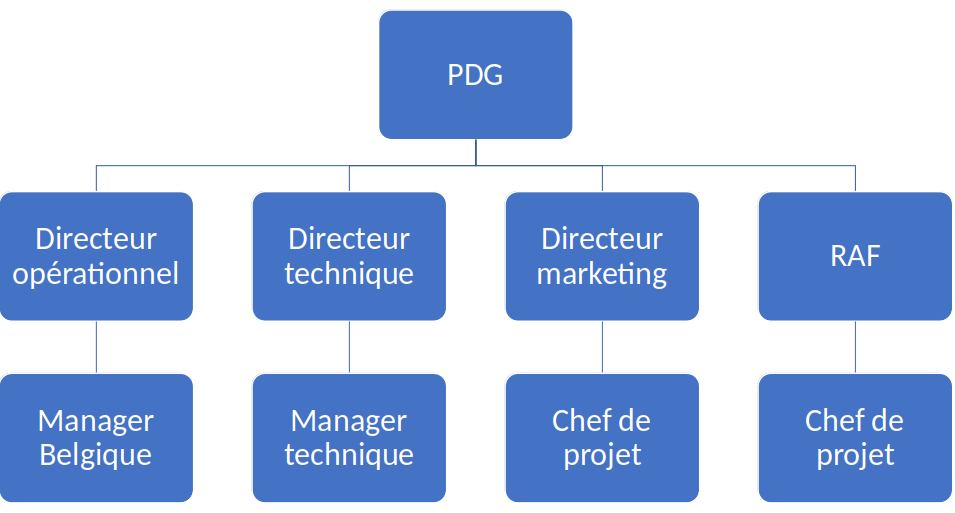
\includegraphics[scale=0.8,width=400px]{./Template LaTeX/Images/og.png}
	\centering
	\caption{Organigramme du CADORIM}
\end{figure}
\begin{comment}
	content...

\subsection{Planification du projet}
J'effectuais le diagramme de Gantt, pour avoir une meilleure compréhension de la chronologie des étapes de mon projet.
\newline
\newline
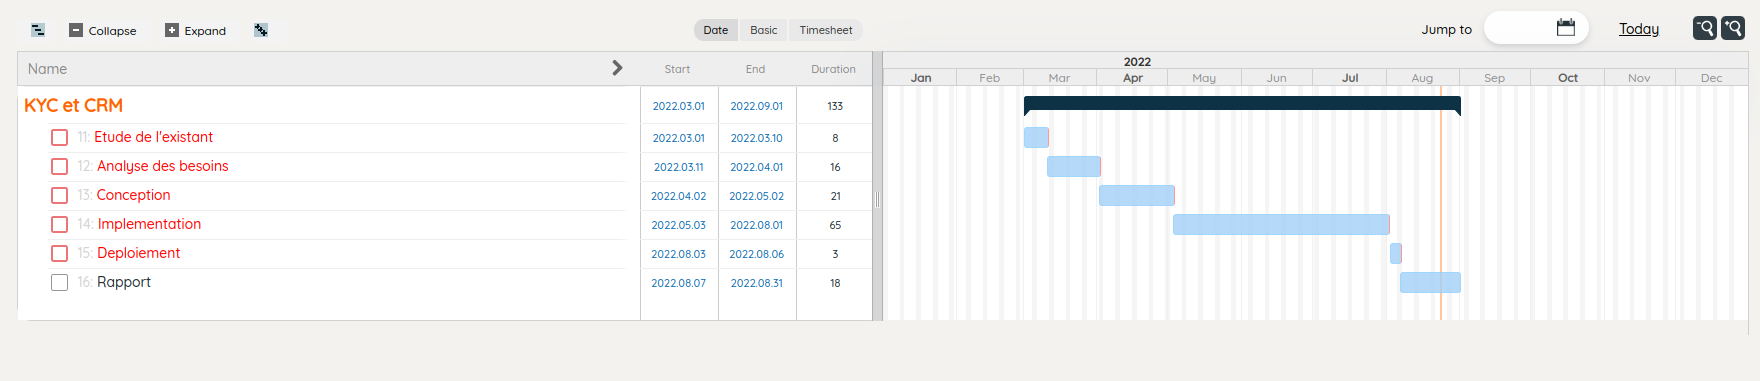
\includegraphics[width=500px,height=175px]{./Template LaTeX/Images/gantt.png}
\newline
Le projet est subdivisé en plusieurs phases.
\begin{enumerate}
\item Une phase comprenant l’étude de l’existant et analyse des besoins, en
intervenant les différents acteurs du projet.
\item Une phase de conception consistant à modéliser et formaliser les
données brutes du cahier de charge
\item Une phase d’implémentation consiste à traduire techniquement les
données provenant de la conception.
\item Déploiement : externalisation des ressources.
\end{enumerate}
\end{comment}
\newpage
\section{Description du projet}
%%%%%%%%%%%%%%%%%%%%%%%%%%%%%%%%%%%%% New add from Introduction %%%%%%%%%%%%%%%%%%%%%
\begin{comment}
	content...

Savoir qui est votre client et adopter des protocoles pour prévenir la criminalité financière sont des défis permanents pour les institutions financières. De manière significative, les institutions financières (y compris les banques, les coopératives de crédit et les sociétés financières du Fortune 50) doivent se conformer à un ensemble des réglementations de plus en plus complexes pour la vérification de l'identité des clients appelée KYC.

KYC, également connu sous le nom de "Know Your Customer" ou "Know Your Client", est un ensemble de procédures permettant de vérifier l'identité d'un client avant ou pendant les transactions avec les banques et autres institutions financières. Le respect des réglementations KYC peut aider à tenir à distance le blanchiment d'argent, le financement du terrorisme et d'autres stratagèmes de fraude courants. En vérifiant d'abord l'identité et les intentions d'un client au moment de l'ouverture du compte, puis en comprenant ses habitudes de transaction, les institutions financières sont en mesure d'identifier plus précisément les activités suspectes. 

Les institutions financières sont soumises à des normes de plus en plus strictes en matière de lois KYC. Ils doivent dépenser plus d'argent pour se conformer à KYC ou être passibles de lourdes amendes. Ces réglementations signifient que presque toutes les entreprises, plateformes ou organisations qui interagissent avec une institution financière pour ouvrir un compte ou effectuer des transactions devront se conformer à ces obligations.

La gestion de la relation client (CRM) est la combinaison de pratiques, de stratégies et de technologies que les entreprises utilisent pour gérer et analyser les interactions et les données client tout au long du cycle de vie du client. L'objectif est d'améliorer les relations de service client, de contribuer à la fidélisation de la clientèle et de stimuler la croissance des ventes. Les systèmes CRM compilent les données client à travers différents canaux, ou points de contact, entre le client et l'entreprise, qui peuvent inclure le site Web de l'entreprise, le téléphone, le chat en direct, le publipostage, les supports marketing et les réseaux sociaux. Les systèmes CRM peuvent également donner aux membres du personnel en contact avec les clients des informations détaillées sur les informations personnelles des clients, l'historique des achats, les préférences et les préoccupations d'achat.


\subsection{Motivations}    

KYC est un moyen de rendre la vérification de l'identité des clients plus précise et moins vulnérable à la fraude.

KYC doivent être effectuées lors de l'intégration d'un nouveau client, mais il est préférable de répéter ces vérifications de temps en temps, pour s'assurer que tout est comme il se doit. En surveillant les comptes clients de cette manière, les comportements suspects peuvent être signalés plus rapidement.

Un système CRM fournit des flux de travail automatisés qui permettent à votre équipe marketing de consacrer plus de temps à des tâches stratégiques, telles que la création de campagnes marketing qui résonnent, l'analyse des données de ces campagnes et le test de différentes approches basées sur ces analyses. Les agents du service client peuvent passer leur temps à travailler avec des clients qui ont des questions, des problèmes ou des besoins plus complexes. En bref, avec des processus de service client plus efficaces, les entreprises peuvent établir de meilleures relations avec leurs clients.
\end{comment}
\subsection{Problématiques}	

En réalité, la réalisation d'une application,qui applique le principe de KYC et integre un  système CRM,
nécessite
de faire face à des problématiques diverses et complexes. Ainsi, la société a décidé de se contenter,
dans un premier temps, Mise en place d’un système d’extration des donnees à partir des images (carte d'identité ou passeport) et traitement des ces donnees.
Ce sujet soulève de nombreuses questions aux implications différentes. Comment peut extraire le texte apartir de l'image? Comment sera-t-il traité ? Comment peut-il être utilisé dans le principe KYC ? Comment pouvons-nous obtenir un système CRM intégré ?


\subsection{Objectifs}

La mise en place d'une application pour appliquer l'ide de KYC en basant sur les différent technologie disponible . En basan sur l'extraction du text apartir d'une imange OCR on peut extracter la code MRZ apartir d'une imange du piece d'idendite ou passport est passe le code a un algorithem qui permer de d'etecter les information personnel.





	%\chapter{Analyse et Spécification des Besoins}
\label{sec:Analyse et Spécification des Besoins}
\section{Introduction}
\section{User expérience}
\section{Différence entre UX et UI}
\section{Mise en place du processus}
\subsection{L’atelier (workshop)}
	%\chapter{Conception du projet}
%\label{sec:EnvironnementDeTravail}
\chapter{Analyse fonctionnelle et conceptuelle}
\label{sec:Analyse fonctionnelle et conceptuelle}
%Durant la réalisation de ce projet, nous avons essayé d’utiliser différents
%outils de développement, d’une part afin de rendre la tâche de la
%réalisation plus facile, d’autre part pour que notre système soit robuste et
%répond parfaitement a nos besoins , et que nos interfaces soient claires et
%faciles à utiliser.

%\section{Choix de langage de modélisation :}
\section{Analyse fonctionnelle}
%Dans cette section, je présente le langage et le logiciel de modélisation que j’ai utilisé pour concevoir notre solution.
\begin{comment}
	content...

\subsection{UML}
On a utilisé UML comme langage de modélisation.
Langage de modélisation unifié UML (Unified modeling Langage) un
consiste a modéliser une application logicielle d'une façon standard
dans le cadre de conception orientée objet.
UML consiste a couvrir le cycle de vie d'un logiciel depuis la
spécification des besoins jusqu'au codage en offrant plusieurs
moyens de description et de modélisation des acteurs.
\section{Choix de logiciel de modélisation :}
\subsection{Visual Paradigm  en ligne} 
Visual Paradigm  en ligne est un outil de création de diagrammes en ligne. Vous pouvez créer un nombre illimité de diagrammes, graphiques et autres visuels à partir d’un large éventail de types de diagrammes, y compris UML, organigrammes, BPMN, ERD, DFD, ArchiMate et autres.
%%%%%%%%%%%%%%%%%%%%%%%%%%%%%%%%%%%%%%%%%%%%%%%%%%%%%%%%% Tests %%%%%%%%%%%%%%%%%%%%%%%%%%
\section{Diagramme UML}
\begin{comment}
\begin{table}
		
	\caption{Rôles des diagrammes UML utilisés.}
	\label{table:kysymys}
\begin{tabular}{|c|p{11cm}|}
	
	\hline
	\large \bfseries Diagramme & \large \bfseries Rôle\\
	\hline
	Diagramme de cas d’utilisation & Il consiste à donner une vision globale sur les principales fonctionnalités
	(chaque fonctionnalité représente un cas d’utilisateur) d’une application .  \\
	\hline
	Diagramme d’activité &  Fournir une vue du comportement d'un système en décrivant la séquence d'actions d'un processus.    \\
	\hline
	Diagramme de séquence &Permettent d'identifier les classes requises par un système et le comportement des objets de classes au cours des interactions.  \\
	\hline
	Diagramme de classe    &Le diagramme de classes représente généralement un schéma utilisé en génie
	logiciel pour modéliser un problème bien précis, sous forme des classes et des
	interfaces ainsi que les différentes relations entre celles-ci. \\
	\hline
	
\end{tabular}

\end{table}
\end{comment}
%Table \ref{table:kysymys} on page \pageref{table:kysymys} refers to the ...

\subsection{Diagramme de cas d’utilisation}
\begin{figure}[h!]
	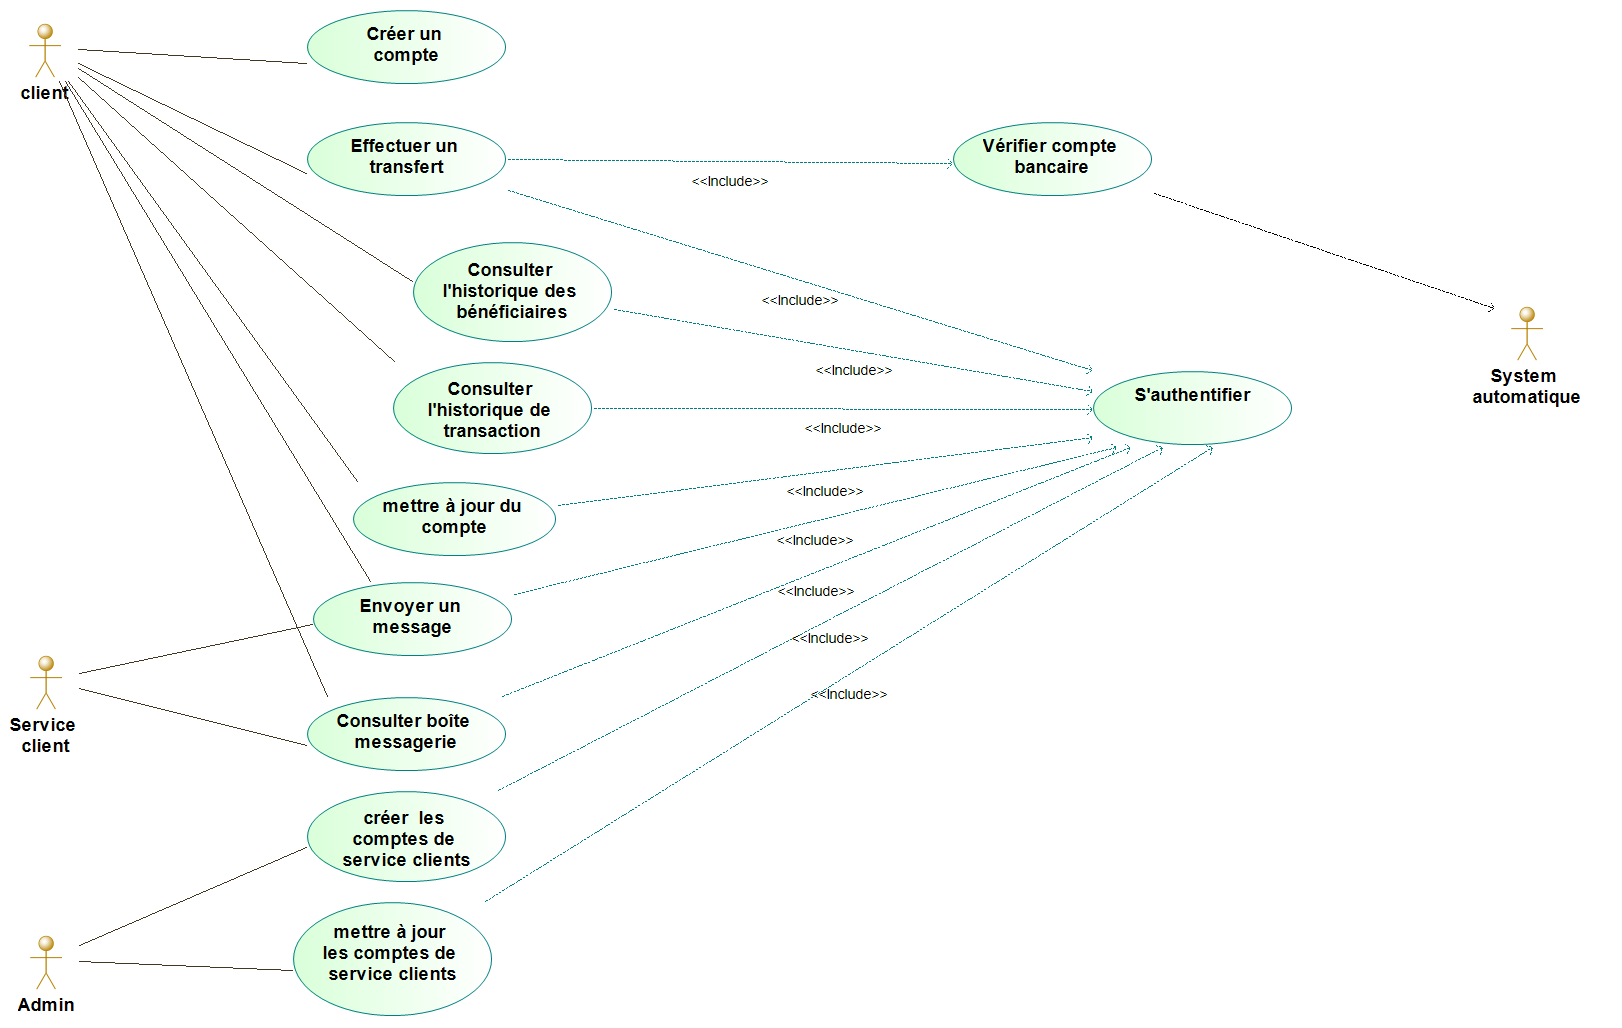
\includegraphics[width=18cm, height=12cm]{./Template LaTeX/Images/use_case.png}
	\caption{Diagramme de cas d’utilisation.}
	\label{fig1:use_case}
\end{figure}
%\textbf{Description détaillée des cas d'utilisation :}
\begin{comment}

\begin{table}[h]
	\begin{tabular}{|m{5cm}|m{2cm}|m{10cm}|}
		\hline
		\textbf{Cas d’utilisation} & \textbf{Acteur} & \textbf{Description}\\
		\hline
		\textbf{Créer un compte }&Client&L'utilisateur se renseigne pour créer un compte au sein de Cadorim pour
		pouvoir accéder au fonctionnalités proposées .\\
		\hline
		\textbf{S’authentifier}&Client&L'utilisateur saisit son identifiant et son mot de passe pour
		accéder aux fonctionnalités.\\
		\hline
		\textbf{Effectuer un transfert}&Client&L'utilisateur saisi le numéro du bénéficiaire et le montant a transférer.
		Une page de vérification avec les informations saisies.
		Transfère le montant vers le bénéficiaire.\\
		\hline
		\textbf{Créer un compte}&Client&L'utilisateur se renseigne pour créer un compte au sein de mauripay pour
		pouvoir accéder au fonctionnalités proposées .\\
		\hline
		\textbf{Créer un compte}&Client&L'utilisateur se renseigne pour créer un compte au sein de mauripay pour
		pouvoir accéder au fonctionnalités proposées .\\
		\hline
		\textbf{Créer un compte}&Client&L'utilisateur se renseigne pour créer un compte au sein de mauripay pour
		pouvoir accéder au fonctionnalités proposées .\\
		\hline
		
	
			
	\end{tabular}
	\caption{Description détaillée des cas d'utilisation}
	\label{4.1}
\end{table}
\end{comment}


	%\textbf{• Description détaillée des cas d'utilisation  :}
\begin{comment}
	
\begin{table}[h]
	\begin{tabular}{|m{4cm}|m{13.5cm}|}
		\hline
		\textbf{Cas d’utilisation}   \textbf{Description}\\
		\hline
		Créer un compte&L'utilisateur se renseigne pour créer un compte au sein de Cadorim pour
		pouvoir accéder au fonctionnalités proposées .\\
		\hline
		S’authentifier&L'utilisateur saisit son identifiant et son mot de passe pour
		accéder aux fonctionnalités.\\
		\hline
		Effectuer un transfert&L'utilisateur saisi le montant a transférer et les informations de  bénéficiaire.
		\newline Une page de vérification avec les informations saisies.
		\newline Transfère le montant vers le bénéficiaire.\\
		\hline
		Consulter l'historique des bénéficaires&L'utilisateur peut voire liste des bénéficaires \\
		\hline
		Consulter l'historique des transactions&L'utilisateur peut voire liste des transactions\\
		\hline
		mettre à jour du compte&L'utilisateur se renseigne pour créer un compte au sein de mauripay pour
		pouvoir accéder au fonctionnalités proposées .\\
		\hline
		Envoyer un message&L'utilisateur se renseigne pour créer un compte au sein de mauripay pour
		pouvoir accéder au fonctionnalités proposées .\\
		\hline
			Consulter boite \newline messagerie&L'utilisateur se renseigne pour créer un compte au sein de mauripay pour
		pouvoir accéder au fonctionnalités proposées .\\
		\hline
		
		
		
	\end{tabular}
	\caption{Description détaillée des cas d'utilisation d'acteur client}
	\label{4.1}
\end{table}
	content...
\end{comment}
%\newpage
\textbf{\hspace*{-1cm}• Description détaillée des cas d'utilisation  :\newline}
\begin{table}[h]
	\hspace*{-2cm}
	\begin{tabular}{|m{19.8cm}|}
		\hline
		\begin{center}
		 \textbf{Cas d’utilisation : Créer un compte, S’authentifier et Créer les comptes de service clients }
		\end{center}
		\\
		[-4ex] 
		\hline
			\begin{tabular}{m{3cm}|m{14cm}}
			
				\centering 	\textbf{Titre} & Créer un compte , S’authentifier , Créer les comptes de service clients
				\\
				[0ex] 
			\end{tabular}
		\\
		
		\hline
			\begin{tabular}{m{3cm}|m{14cm}}
			
			\centering 	\textbf{But} & Créer un compte pour accéder aux fonctionnalités de l’application 	\\
			[0ex] 
			
		\end{tabular}
		\\
		\hline
			\begin{tabular}{m{3cm}|m{15.5cm}}
			
			\centering 	\textbf{Résumé} & L'utilisateur doit remplir un formulaire d’inscription et identifier électroniquement leur document comme des pièces d’identité (carte d’identité, passeport ) à partir de leur caméra du téléphone puis valide son action.\newline Le système effectue une vérification puis une mise à jour de la base de données.
			\\
			[0ex] 
		\end{tabular}
		\\
		
		\hline
			\begin{tabular}{m{3cm}|m{14cm}}
			
			\centering 	\textbf{Acteurs } & Client,Admin \\[0ex]
			
		\end{tabular}
		\\
		 
		\hline
		\begin{center}
			\textbf{Descriptions des enchainements}
		\end{center}
		\\
		[-4ex] 
		\hline	
			\begin{tabular}{m{9.3cm}|m{9.3cm}}
			
			\begin{center}
				\textbf{Pré condition}
			\end{center}
		 		& 
		 	\begin{center}
				\textbf{Post condition}
			\end{center}
			\\[-4ex]
		\end{tabular}
		\\
		
		\hline
			\begin{tabular}{m{9.3cm}|m{9.3cm}}
			L'utilisateur doit accéder au système
			& 
			L'utilisateur inscrit
		\end{tabular}
		\\
		\hline
			\begin{center}
			\textbf{Scenario nominal}
			\end{center}
		\\
		[-4ex]
		\hline
		\begin{enumerate}
			\item [1.] L’utilisateur demande la page d’inscription en cliquant sur «S'INSCRIRE»
			\item [2.] Le système lui envoie la page d’inscription
			\item [3.] L’utilisateur rempli le formulaire et scanne leur document puis appuie sur S'INSCRIRE
			\item [4.] Le système effectue les validations et l’enregistrement dans la base de données
			\item [5.] L’utilisateur est redirigé vers la page d’authentification et renseigne ses identifiants en cas d'acteur client 
		\end{enumerate}
		\\
		[-4ex]
		\hline	
			\begin{center}
			\textbf{Enchainement d’échec }
		\end{center}
		\\ 
		[-4ex]
		\hline
		\begin{tabular}{m{17.5cm}}
			\begin{enumerate}
				\item [6.] Le compte existe déjà ou les données saisies sont incorrectes
				\item [7.] Il n’y a pas de connexion internet
			\end{enumerate}
			\\[-4ex]
		\end{tabular}
		\\
		\hline	
		
	\end{tabular}
	\centering \caption{Description détaillée des cas d'utilisation : Créer un compte  et S’authentifier}
	\label{4.1}
\end{table}
\newpage

\begin{table}[h]
	\hspace*{-2cm}
	\vspace*{-2cm}
	\begin{tabular}{|m{19.8cm}|}
		\hline
		\begin{center}
			\textbf{Cas d’utilisation : Effectuer transfert}
		\end{center}
		\\
		[-4ex] 
		\hline
		\begin{tabular}{m{3cm}|m{14cm}}
			
			\centering 	\textbf{Titre} & Effectuer transfert
			\\
			[0ex] 
		\end{tabular}
		\\
		
		\hline
		\begin{tabular}{m{3cm}|m{14cm}}
			
			\centering 	\textbf{But} & Envoyer de l’argent à un bénéficiaire	\\
			[0ex] 
			
		\end{tabular}
		\\
		\hline
		\begin{tabular}{m{3cm}|m{15.5cm}}
			
			\centering 	\textbf{Résumé} & L’utilisateur saisit les informations du bénéficiaire et le montant de la transaction et valide. Le système envoyait les informations de la carte bancaire au  fournisseur de paiement  avant de finaliser l’opération.
			\\
			[0ex] 
		\end{tabular}
		\\
		
		\hline
		\begin{tabular}{m{3cm}|m{14cm}}
			
			\centering 	\textbf{Acteurs } & Client \\[0ex]
			
		\end{tabular}
		\\
		
		\hline
		\begin{center}
			\textbf{Descriptions des enchainements}
		\end{center}
		\\
		[-4ex] 
		\hline	
		\begin{tabular}{m{9.3cm}|m{9.3cm}}
			
			\begin{center}
				\textbf{Pré condition}
			\end{center}
			& 
			\begin{center}
				\textbf{Post condition}
			\end{center}
			\\[-4ex]
		\end{tabular}
		\\
		
		\hline
		\begin{tabular}{m{9.3cm}|m{9.3cm}}
			- L’utilisateur doit se connecter \newline
			- L’utilisateur doit utiliser une carte bancaire valide & 
			- Le transfert est effectué \newline
			- Afficher  l'historique des transactions
			\\[0ex]
		\end{tabular}
		\\
		\hline
		\begin{center}
			\textbf{Scenario nominal}
		\end{center}
		\\
		[-4ex]
		\hline
		\begin{enumerate}
			\item [1.] L’utilisateur accède au formulaire de transfert en saisit le montant puis  cliquant sur « Envoyer »
			\item [2.] Le système lui demande de saisir les informations de transfert
			\item [3.] L’utilisateur rempli le formulaire appuie sur le bouton « Valider »
			\item [4.] Le système débiter le compte de cadorim et crédité le compte de bénéficiaire
			\item [5.] Le système lui affiche la page de l'historique des transactions
		\end{enumerate}
		\\
		[-4ex]
		\hline	
		\begin{center}
			\textbf{Enchainement d’échec }
		\end{center}
		\\ 
		[-4ex]
		\hline
		\begin{tabular}{m{17.5cm}}
			\begin{enumerate}
				\item [6.] La carte bancaire invalide ou le solde est insuffisant
				\item [7.] La saisie de données n’est pas correcte
				\item [8.] La connexion n’est pas bonne pour effectuer et suivre un transfert
			\end{enumerate}
			\\[-4ex]
		\end{tabular}
		\\
		\hline	
		
	\end{tabular}
	\vspace*{1.5cm}
	\centering \caption{Description détaillée des cas d'utilisation : Effectuer transfert}
	\label{4.1}
\end{table}

\newpage

\begin{table}[h]
	\hspace*{-2cm}
	\vspace*{-2.5cm}
	\begin{tabular}{|m{19.8cm}|}
		\hline
		\begin{center}
			\textbf{Cas d’utilisation : Consulter l'historique des bénéficiaires et l'historique de transaction}
		\end{center}
		\\
		[-4ex] 
		\hline
		\begin{tabular}{m{3cm}|m{14cm}}
			
			\centering 	\textbf{Titre} & Consulter l'historique des bénéficiaires,Consulter l'historique de transaction
			\\
			[0ex] 
		\end{tabular}
		\\
		
		\hline
		\begin{tabular}{m{3cm}|m{14cm}}
			
			\centering 	\textbf{But} & Consultations de l'historique\\
			[0ex] 
			
		\end{tabular}
		\\
		\hline
		\begin{tabular}{m{3cm}|m{15.5cm}}
			
			\centering 	\textbf{Résumé} & L'utilisateur voit les renseignements sur le bénéficiaire et l'opération de transaction.
			\\
			[0ex] 
		\end{tabular}
		\\
		
		\hline
		\begin{tabular}{m{3cm}|m{14cm}}
			
			\centering 	\textbf{Acteurs } & Client \\[0ex]
			
		\end{tabular}
		\\
		
		\hline
		\begin{center}
			\textbf{Descriptions des enchainements}
		\end{center}
		\\
		[-4ex] 
		\hline	
		\begin{tabular}{m{9.3cm}|m{9.3cm}}
			
			\begin{center}
				\textbf{Pré condition}
			\end{center}
			& 
			\begin{center}
				\textbf{Post condition}
			\end{center}
			\\[-4ex]
		\end{tabular}
		\\
		
		\hline
		\begin{tabular}{m{9.3cm}|m{9.3cm}}
			- L’utilisateur doit se connecter \newline
			 & 
			- Afficher  l'historique des transactions ou des  \newline bénéficiaires
			\\[0ex]
		\end{tabular}
		\\
		\hline
		\begin{center}
			\textbf{Scenario nominal}
		\end{center}
		\\
		[-4ex]
		\hline
		\begin{enumerate}
			\item [1.] L’utilisateur accède a l'historique des transactions ou des bénéficiaires en cliquant sur « Transferts » ou « Benef »
			\item [2.] Le système lui affiche la page de l'historique
		\end{enumerate}
		\\
		[-4ex]
		\hline	
		\begin{center}
			\textbf{Enchainement d’échec }
		\end{center}
		\\ 
		[-4ex]
		\hline
		\begin{tabular}{m{17.5cm}}
			\begin{enumerate}
				\item [3.] Il n’y a pas de connexion internet
				
			\end{enumerate}
			\\[-4ex]
		\end{tabular}
		\\
		\hline	
		
	\end{tabular}
	\vspace*{2cm}
	\centering \caption{Description détaillée des cas d'utilisation : Consulter l'historiques(des transactions ou des bénéficiaires)}
	\label{4.1}
\end{table}

\newpage

\begin{table}[h]
	\hspace*{-2cm}
	\vspace*{-2cm}
	\begin{tabular}{|m{19.8cm}|}
		\hline
		\begin{center}
			\textbf{Cas d’utilisation : Consulter boite messagerie}
		\end{center}
		\\
		[-4ex] 
		\hline
		\begin{tabular}{m{3cm}|m{14cm}}
			
			\centering 	\textbf{Titre} & Consulter boite messagerie
			\\
			[0ex] 
		\end{tabular}
		\\
		
		\hline
		\begin{tabular}{m{3cm}|m{14cm}}
			
			\centering 	\textbf{But} & Consulter boite messagerie\\
			[0ex] 
			
		\end{tabular}
		\\
		\hline
		\begin{tabular}{m{3cm}|m{15.5cm}}
			
			\centering 	\textbf{Résumé} &L'utilisateur voit l'historique des  messages et les messages reçus.
			\\
			[0ex] 
		\end{tabular}
		\\
		
		\hline
		\begin{tabular}{m{3cm}|m{14cm}}
			
			\centering 	\textbf{Acteurs } & Client, Srvice client \\[0ex]
			
		\end{tabular}
		\\
		
		\hline
		\begin{center}
			\textbf{Descriptions des enchainements}
		\end{center}
		\\
		[-4ex] 
		\hline	
		\begin{tabular}{m{9.3cm}|m{9.3cm}}
			
			\begin{center}
				\textbf{Pré condition}
			\end{center}
			& 
			\begin{center}
				\textbf{Post condition}
			\end{center}
			\\[-4ex]
		\end{tabular}
		\\
		
		\hline
		\begin{tabular}{m{9.3cm}|m{9.3cm}}
			- L’utilisateur doit se connecter \newline
			& 
			- Afficher  l'historique des  messages et les messages reçus
			\\[0ex]
		\end{tabular}
		\\
		\hline
		\begin{center}
			\textbf{Scenario nominal}
		\end{center}
		\\
		[-4ex]
		\hline
		\begin{enumerate}
			\item [1.] L’utilisateur accède à la boîte messagerie
			\item [2.] Le système lui affiche la page des messageries
		\end{enumerate}
		\\
		[-4ex]
		\hline	
		\begin{center}
			\textbf{Enchainement d’échec }
		\end{center}
		\\ 
		[-4ex]
		\hline
		\begin{tabular}{m{17.5cm}}
			\begin{enumerate}
				\item [3.] Il n’y a pas de connexion internet
				
			\end{enumerate}
			\\[-4ex]
		\end{tabular}
		\\
		\hline	
		
	\end{tabular}
	\vspace*{1.5cm}
	\centering \caption{Description détaillée des cas d'utilisation : Consulter boite messagerie}
	\label{4.1}
\end{table}


\newpage

\begin{table}[h]
	\hspace*{-2cm}
	\vspace*{-2cm}
	\begin{tabular}{|m{19.8cm}|}
		\hline
		\begin{center}
			\textbf{Cas d’utilisation : Envoyer un message}
		\end{center}
		\\
		[-4ex] 
		\hline
		\begin{tabular}{m{3cm}|m{14cm}}
			
			\centering 	\textbf{Titre} & Envoyer un message
			\\
			[0ex] 
		\end{tabular}
		\\
		
		\hline
		\begin{tabular}{m{3cm}|m{14cm}}
			
			\centering 	\textbf{But} & Envoyer un message\\
			[0ex] 
			
		\end{tabular}
		\\
		\hline
		\begin{tabular}{m{3cm}|m{15.5cm}}
			
			\centering 	\textbf{Résumé} &L'utilisateur peut envoyer un message où répond à un message
			\\
			[0ex] 
		\end{tabular}
		\\
		
		\hline
		\begin{tabular}{m{3cm}|m{14cm}}
			
			\centering 	\textbf{Acteurs } & Client, Srvice client \\[0ex]
			
		\end{tabular}
		\\
		
		\hline
		\begin{center}
			\textbf{Descriptions des enchainements}
		\end{center}
		\\
		[-4ex] 
		\hline	
		\begin{tabular}{m{9.3cm}|m{9.3cm}}
			
			\begin{center}
				\textbf{Pré condition}
			\end{center}
			& 
			\begin{center}
				\textbf{Post condition}
			\end{center}
			\\[-4ex]
		\end{tabular}
		\\
		
		\hline
		\begin{tabular}{m{9.3cm}|m{9.3cm}}
			- L’utilisateur doit se connecter \newline
			& 
			\centering - Le message est envoyé
			\\[0ex]
		\end{tabular}
		\\
		\hline
		\begin{center}
			\textbf{Scenario nominal}
		\end{center}
		\\
		[-4ex]
		\hline
		\begin{enumerate}
			\item [1.] L’utilisateur demande le formulaire d’envoi de message
			\item [2.] Le système lui affiche la page des discussions
		\end{enumerate}
		\\
		[-4ex]
		\hline	
		\begin{center}
			\textbf{Enchainement d’échec }
		\end{center}
		\\ 
		[-4ex]
		\hline
		\begin{tabular}{m{17.5cm}}
			\begin{enumerate}
				\item [3.] Il n’y a pas de connexion internet
				
			\end{enumerate}
			\\[-4ex]
		\end{tabular}
		\\
		\hline	
		
	\end{tabular}
	\vspace*{1.5cm}
	\centering \caption{Description détaillée des cas d'utilisation : Envoyer un message}
	\label{4.1}
\end{table}
\begin{comment}

	\item[•]  \textbf{Description détaillée des cas d'utilisation d'acteur service client :}
\begin{table}[h]
	\begin{tabular}{|m{4cm}|m{13.5cm}|}
		\hline
		\textbf{Cas d’utilisation}  & \textbf{Description}\\
		\hline
		Enoyer un message&L'utilisateur se renseigne pour créer un compte au sein de Cadorim pour
		pouvoir accéder au fonctionnalités proposées .\\
		\hline
		S’authentifier&L'utilisateur saisit son identifiant et son mot de passe pour
		accéder aux fonctionnalités.\\
		\hline
			Consulter boite \newline messagerie&L'utilisateur saisit son identifiant et son mot de passe pour
		accéder aux fonctionnalités.\\
		\hline
	\end{tabular}
	\caption{Description détaillée des cas d'utilisation d'acteur service client}
	\label{4.1}
\end{table}

	\item[•]  \textbf{Description détaillée des cas d'utilisation d'acteur admin :}
\begin{table}[h]
	\begin{tabular}{|m{4cm}|m{13.5cm}|}
		\hline
		\textbf{Cas d’utilisation}  & \textbf{Description}\\
		\hline
		Créer les comptes de service clients&L'utilisateur se renseigne pour créer un compte au sein de Cadorim pour
		pouvoir accéder au fonctionnalités proposées .\\
		\hline
		S’authentifier&L'utilisateur saisit son identifiant et son mot de passe pour
		accéder aux fonctionnalités.\\
		\hline
		Mettre à jour les comptes de service clients&L'utilisateur saisit son identifiant et son mot de passe pour
		accéder aux fonctionnalités.\\
		\hline
	\end{tabular}
	\caption{Description détaillée des cas d'utilisation d'acteur admin}
	\label{4.1}
\end{table}
\item[•]  \textbf{Description détaillée des cas d'utilisation d'acteur system :}
\begin{table}[h]
	\begin{tabular}{|m{4cm}|m{13.5cm}|}
		\hline
		\textbf{Cas d’utilisation}  & \textbf{Description}\\
		\hline
		 Vérifier compte \newline bancaire&L'utilisateur se renseigne pour créer un compte au sein de Cadorim pour
		pouvoir accéder au fonctionnalités proposées .\\
		\hline
	\end{tabular}
	\caption{Description détaillée des cas d'utilisation d'acteur secondaire system}
	\label{4.1}
\end{table}
	content...
\end{comment}


\subsection{Diagramme d’activité}
Cette section a pour objectif de mettre en surbrillance le processus quelques fonctionnalités de
l’application pour voir les détailles. J’ai choisi trois cas d’utilisation, à savoir, la création d’un compte,la transfert d'argent et l'authentification.
\newpage
\subsubsection{Création de compte}
Le diagramme d’activité qu’illustre la figure~\ref{activiteCompte} décrit le cas d’utilisation « Créer un compte ».
\begin{figure}[h!]
	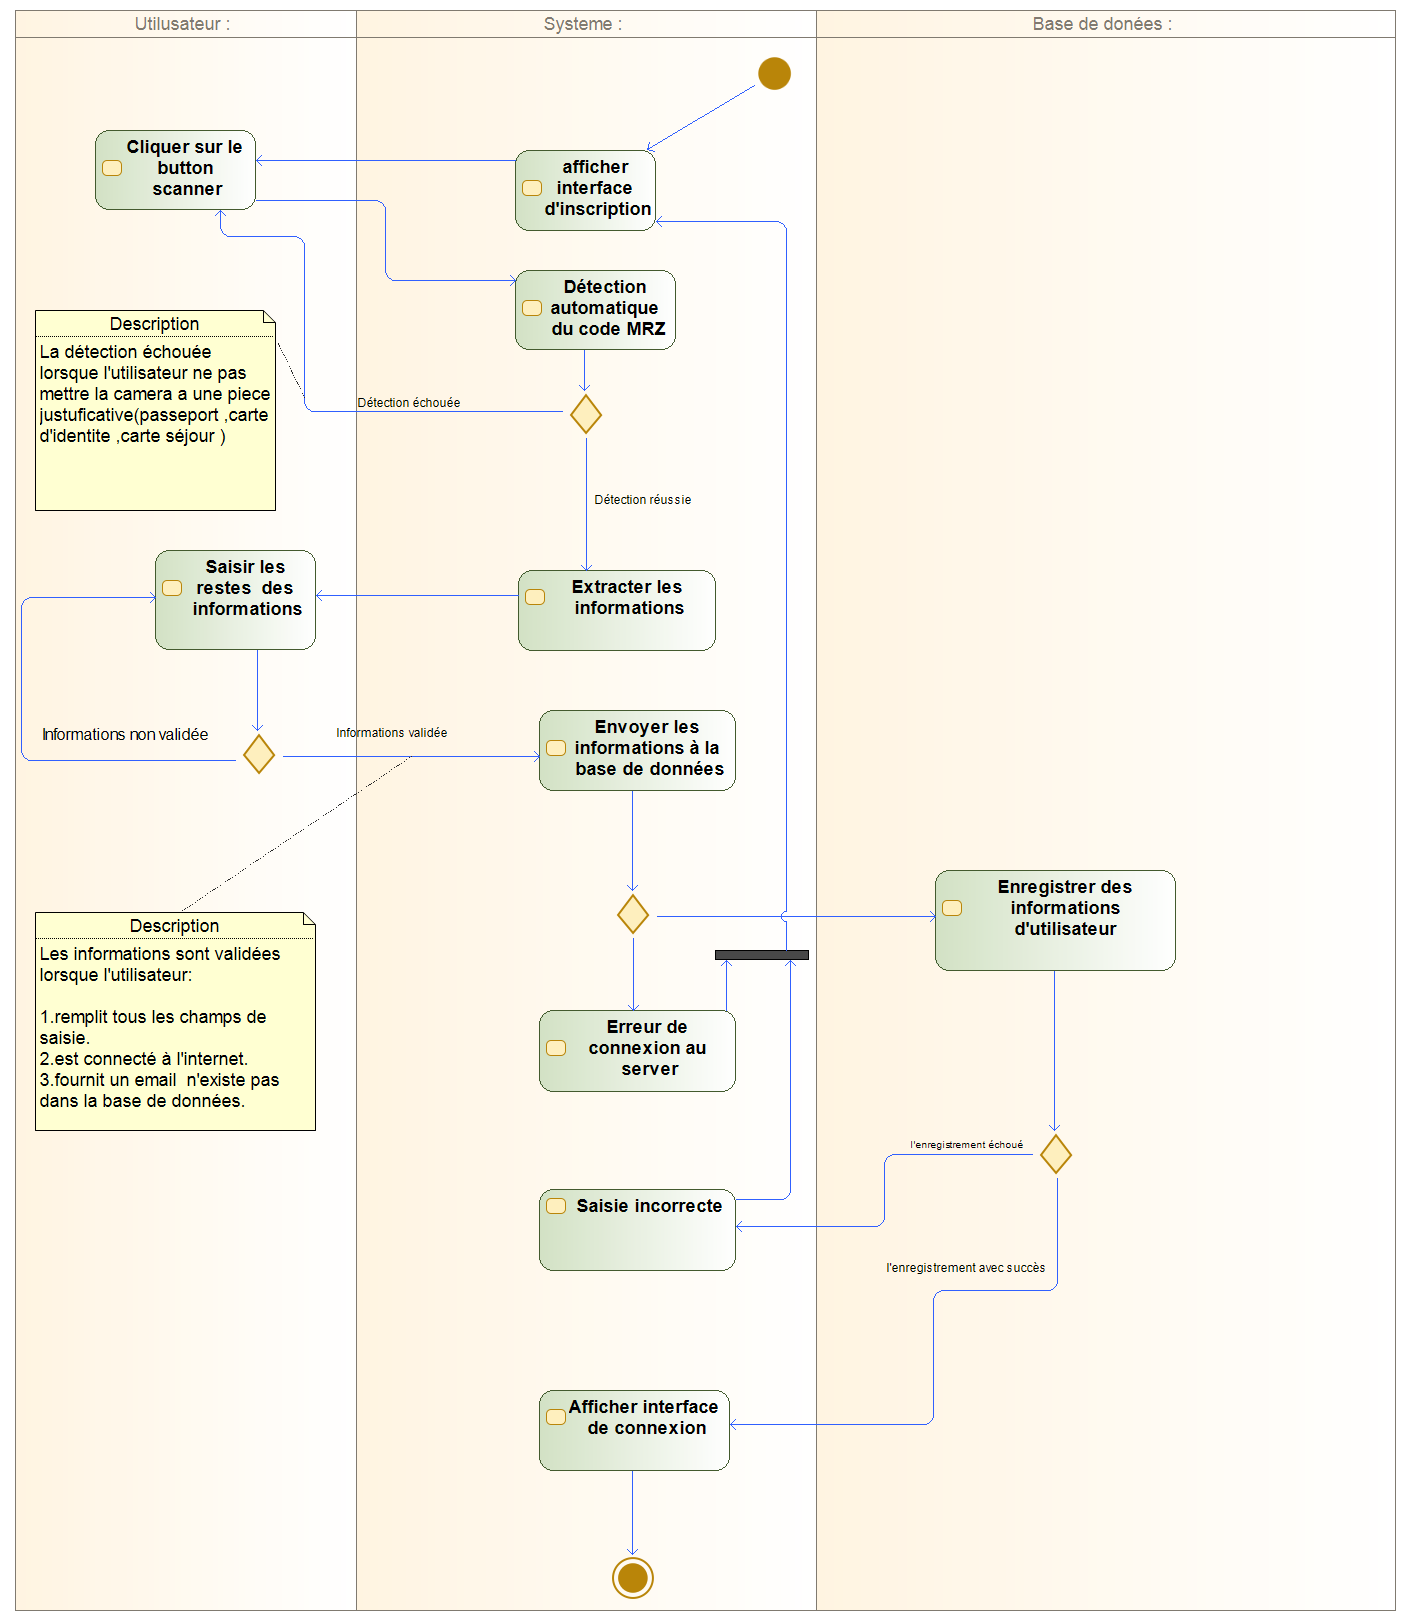
\includegraphics[width=18cm, height=19cm]{./Template LaTeX/Images/ins_act.png}
\caption{Diagramme d’activité : Création de compte}
\label{activiteCompte}

\end{figure}

\subsubsection{Transfert d'argent}
Le diagramme d’activité qu’illustre la figure~\ref{activiteTr} décrit les différentes actions ou enchainements
effectués lors d’une opération de transfert d’argent.
\begin{figure}[h!]
	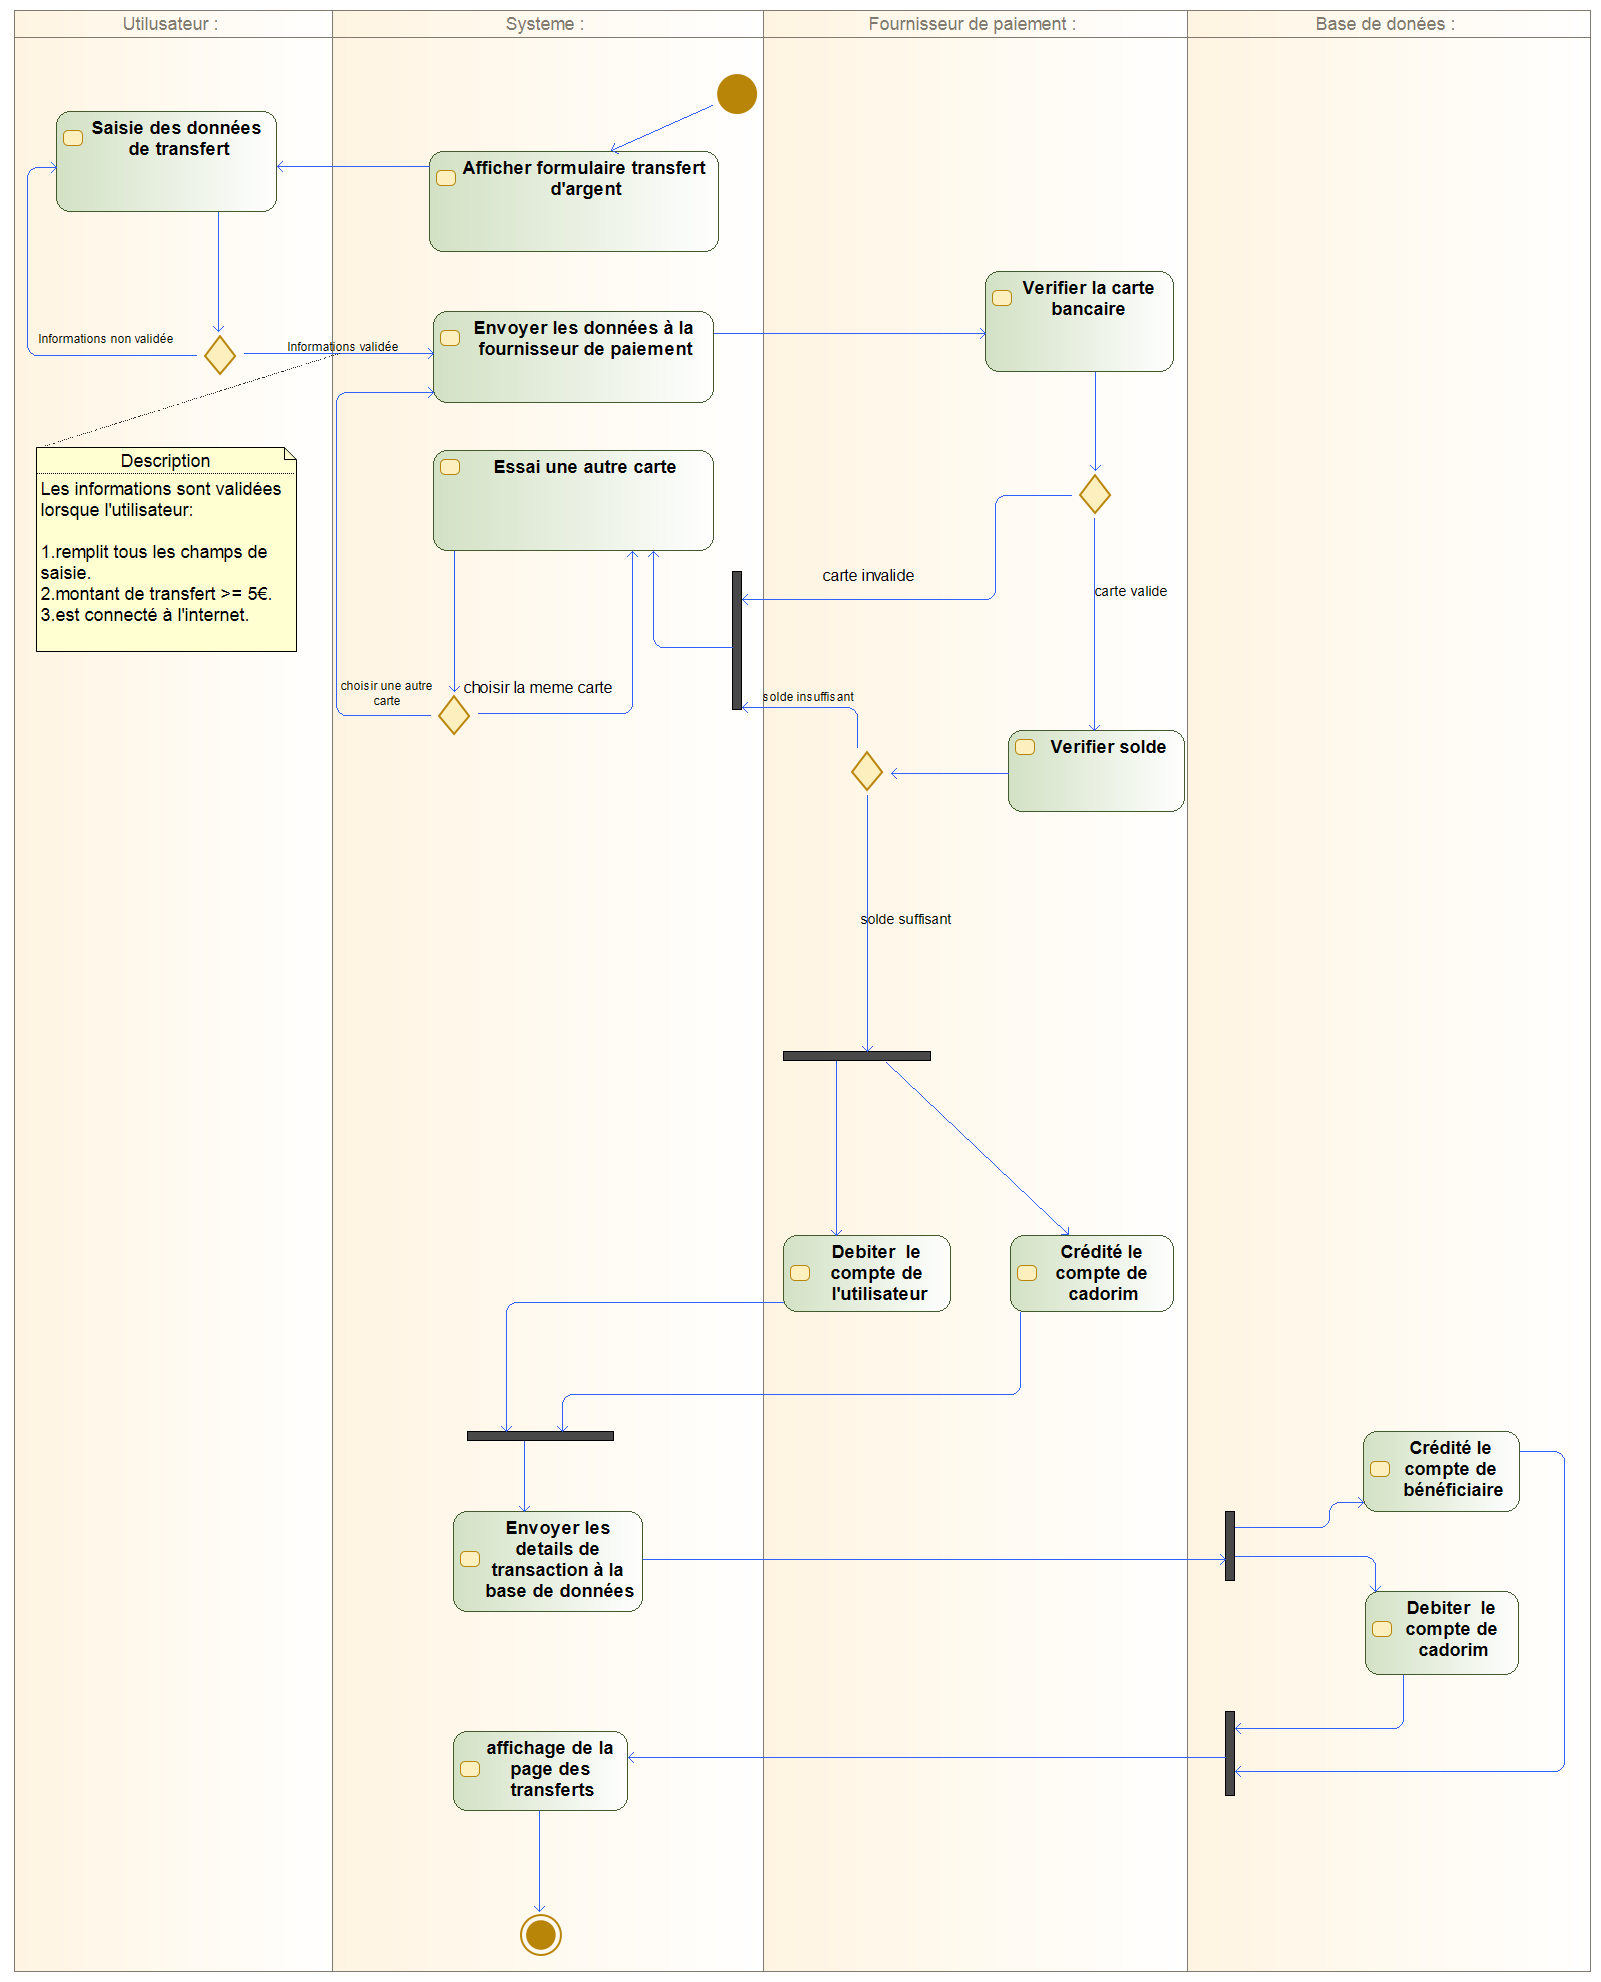
\includegraphics[width=18cm, height=20cm]{./Template LaTeX/Images/trans_act.png}
	\caption{Diagramme d'activité : Transfert d'argent}
	\label{activiteTr}
\end{figure}

\subsubsection{Authentification}
Le diagramme d’activité qu’illustre la figure~\ref{activiteAuth} décrit le cas d’utilisation « Authentification ».
\begin{figure}[h!]
	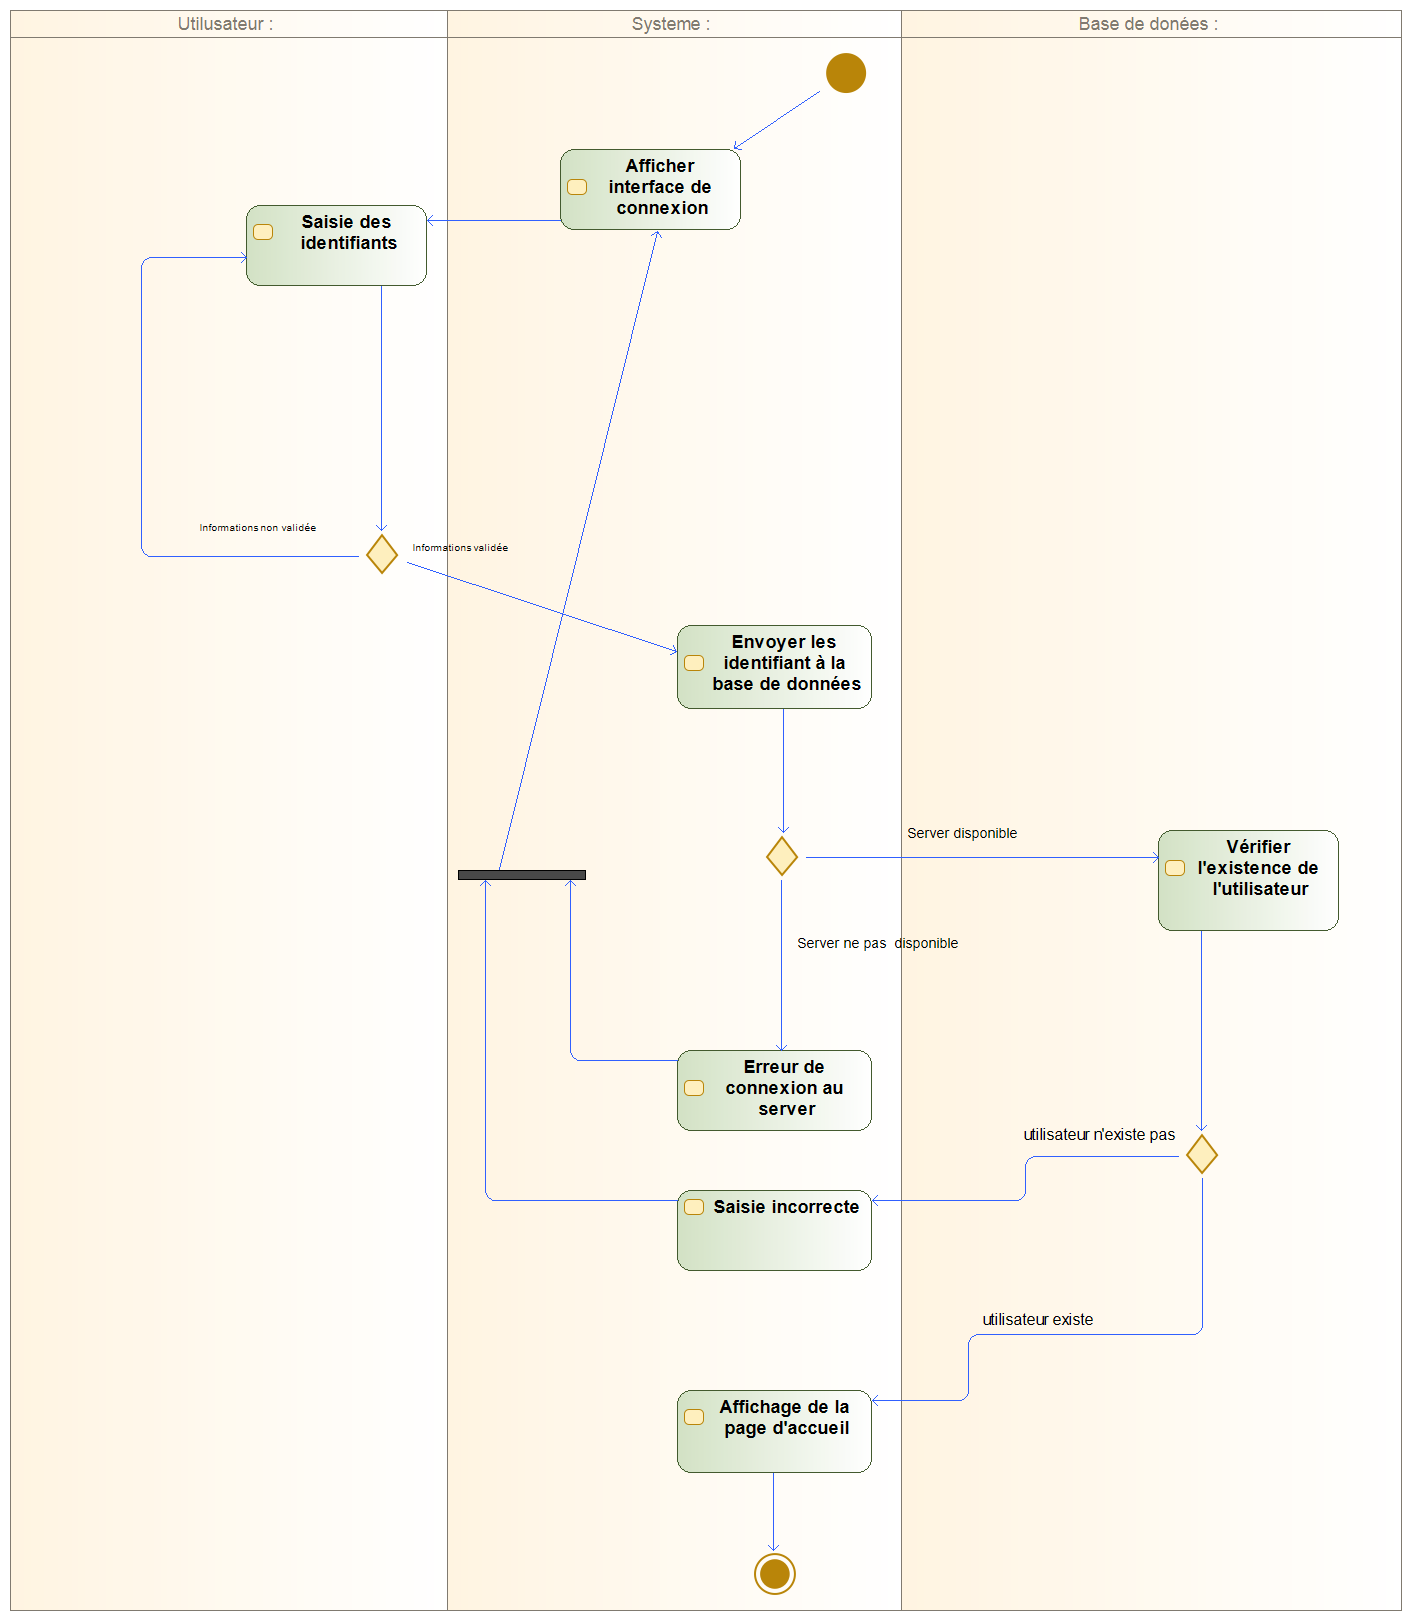
\includegraphics[width=18cm, height=20cm]{./Template LaTeX/Images/auth_act.png}
	\caption{Diagramme d'activité : Authentification}
	\label{activiteAuth}
\end{figure}


%\section{Modélisation de la base de données}
%\subsection{Diagramme de séquence}
%\newpage

\subsection{Diagramme de classe}
Afin de bien détailler l’architecture de la base de données, nous avons conçu le diagramme de
classe représenté dans la figure~\ref{fig4:class}.
\begin{figure}[h!]
	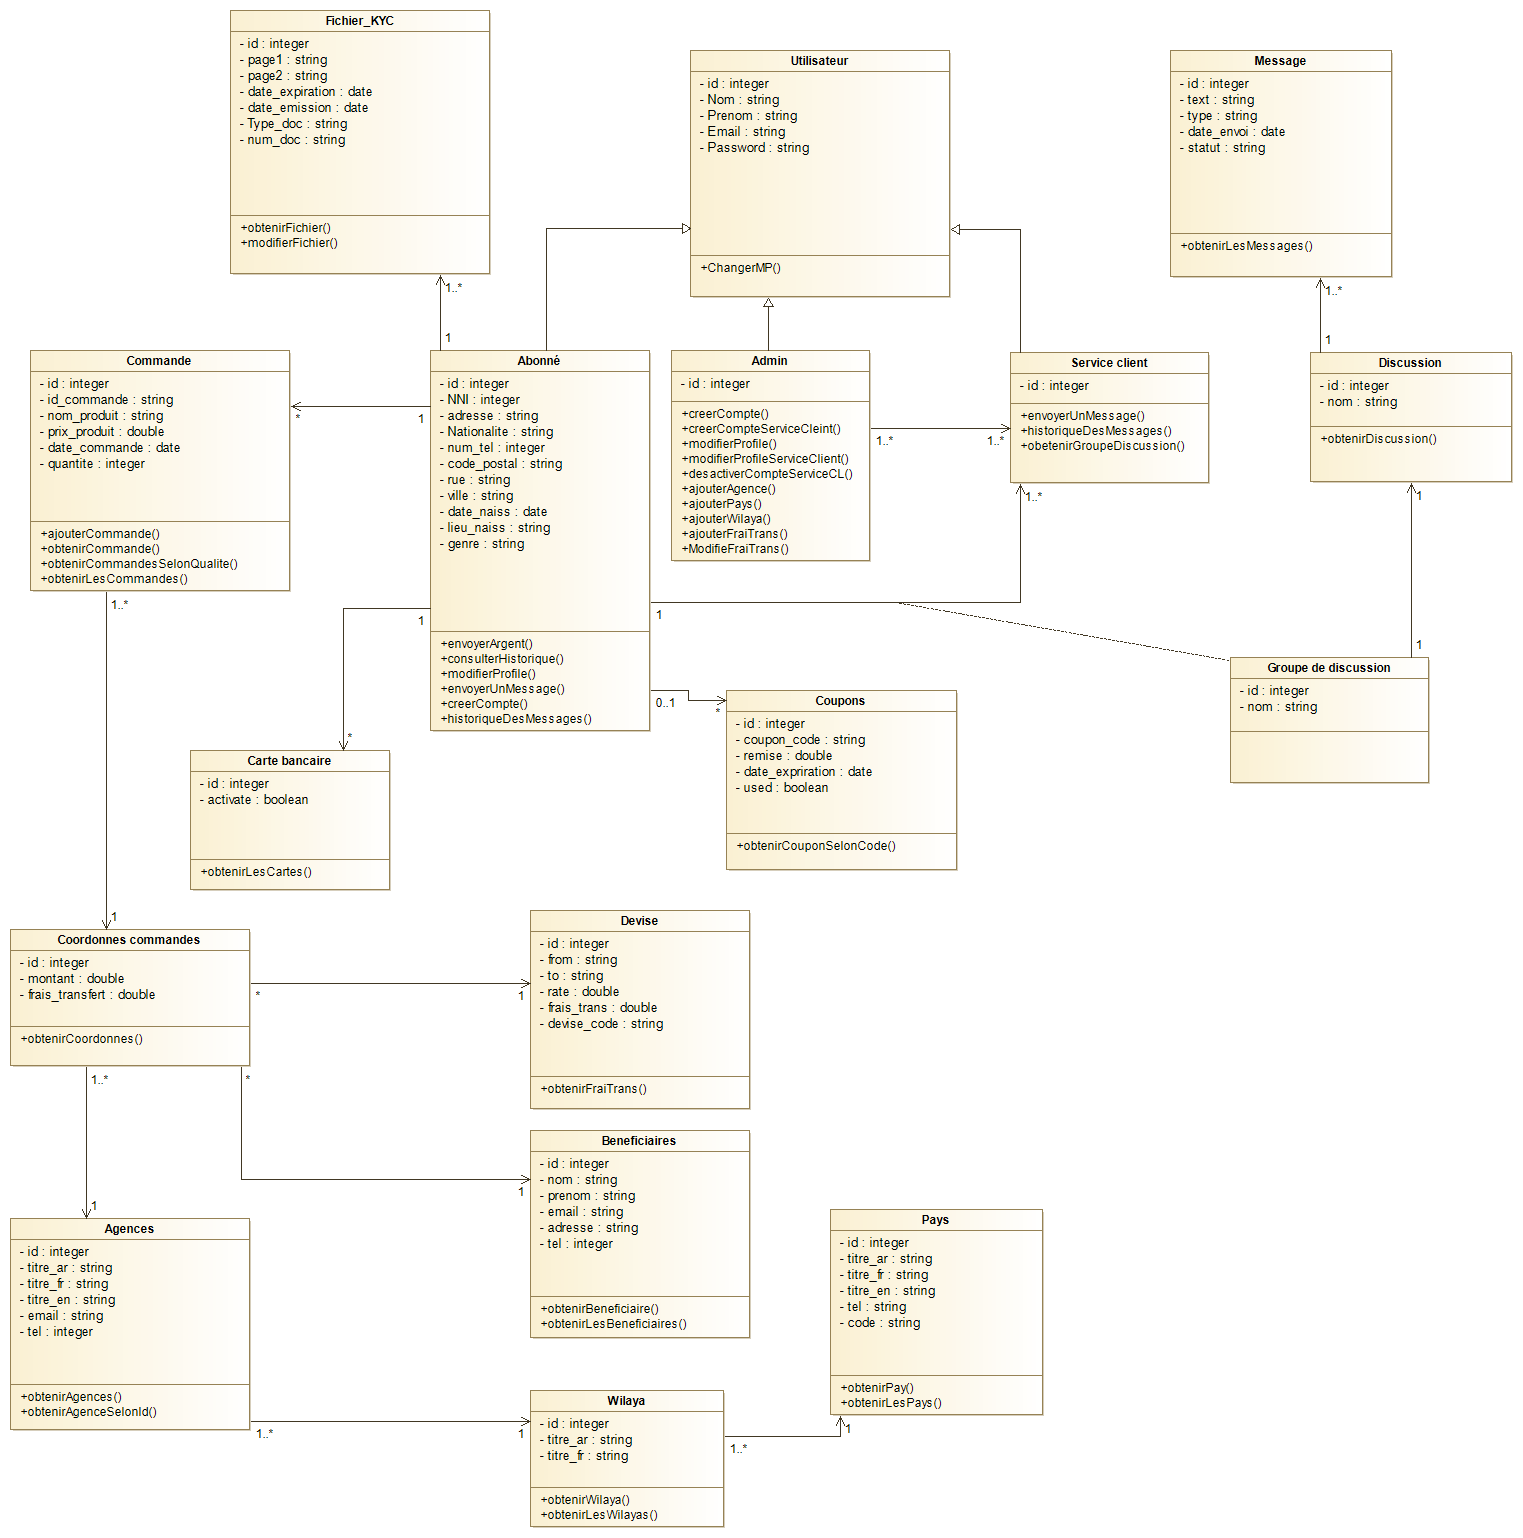
\includegraphics[width=18cm, height=20cm]{./Template LaTeX/Images/Diagramme_de_classe_V3.png}
	\caption{Diagramme de classe}
	\label{fig4:class}
\end{figure}
\newpage
\hspace*{-2cm} Le tableau~\ref{fig4:classT} explique les différentes classes de la base de données.
\begin{table}[h]
	\hspace*{-2cm}
	%\vspace*{6cm}
	\begin{tabular}{|m{5cm}|m{14cm}|}
		\hline
			\textbf{Classe}& \textbf{Description}
		\\
		\hline
		Abonné&Informations de l'utilisateur
		\\
		\hline
		Fichier KYC&  Contient les informations du fichier (carte d'identité, passeport, titre de séjour, carte bancaire) de client
		\\
			\hline
		Commande& Informations concernant une commande
		\\
			\hline
		Coordonnes commandes& Détails de chaque commande
		\\
			\hline
		Agences& Informations sur les agences de cadorim
		\\
			\hline
		Carte bancaire& Gestion de carte bancaire\\
		\hline	
			Devise& Informations sur la devise selon le pays d'envoi et le pays reçoivent
		\\
		\hline
			Beneficiaires&Informations sur les Beneficiaires
		\\
		\hline	
			Wilaya&Informations sur les Wilayas
		\\
		\hline	
			Admin&Informations de l’Admin et ses privilèges
		\\
		\hline	
			Service client&Service client avec certains privilèges
		\\
		\hline	
			Coupons&Informations d’un coupon
		\\
		\hline	
			Groupe de discussion&Informations sur les groupes
		\\
		\hline	
			Discussion&Informations de discussion de chaque groupe
		\\
		\hline		
			Message&Contient les messages de chaque discussion
		\\
		\hline
			Pays&Informations sur les pays
		\\
		\hline		
	\end{tabular}
	%\vspace*{10cm}
	\centering \caption{Description de la base de données}
	\label{fig4:classT}
\end{table}

%%%%%%%%%%%%%%%%%%%%%%%%%%%%%%%%%%%%%%%%%%%%5 ICI %%%%%%%%%%%%%%%%%%%%%%%%%%%%%%%%%%%%%%%%555


	\chapter{L’implémentation}

%\section{Environnement de développement}
\section{Environnement de travail}
Durant la réalisation de ce projet, nous avons essayé d’utiliser différents
outils de développement, d’une part afin de rendre la tâche de la
réalisation plus facile, d’autre part pour que notre système soit robuste et
répond parfaitement a nos besoins , et que nos interfaces soient claires et
faciles à utiliser.
\subsection{Environnement logiciel}

\begin{comment}
	content...

\subsection{Front-end}
C’est le développement coté client autrement dit la
partie du code reçu par le client. On rappelle que le client désigne
un navigateur web.
On a choisi Flutter comme Framework pour développer la partie
front de notre application mobile.
Flutter est un framework de développement d’applications mobiles open source de Google. La principale raison de sa popularité est qu’il prend en charge la création 		   
d’applications multiplateformes. Flutter est également utilisé pour créer des apps interactives qui s’exécutent sur des pages web ou sur le bureau.
\end{comment}
\subsubsection{Editeur de texte : VS Code}
VS Code (Visual Studio Code) est un éditeur de code source réalisé par Microsoft pour Win-
dows, Linux et macOS.Les fonctionnalités incluent la prise en charge du débogage, lacoloration
syntaxique, la saisie semi-automatique intelligente du code, les extraits de code, la refactorisation du
code et Gitintégré. Les utilisateurs peuvent modifier le thème,les raccourcis clavier,les préférences et
installer des extensions qui ajoutent des fonctionnalités supplémentaires.\newline Pour en savoir plus, veillez
visiter le lien : \href{https://en.wikipedia.org/wiki/VisualStudioCode}{https://en.wikipedia.org/wiki/VisualStudioCode}
\subsubsection{IDE : Android Studio}
Android Studio est un environnement de développement pour développer des applications mobiles Android. Il est basé sur IntelliJ IDEA et utilise le moteur de production Gradle. Il peut être téléchargé sous les systèmes d'exploitation Windows, macOS, Chrome OS et Linux.
\newline Pour en savoir plus, veillez
visiter le lien : \href{https://en.wikipedia.org/wiki/AndroidStudio.}{https://en.wikipedia.org/wiki/AndroidStudio.}
\subsubsection{Git}
Git est un système de contrôle de version distribué gratuit et Open Source conçu pour gérer des
petits projets aux très grands projets avec rapidité et efficacité. C'est un logiciel libre créé par
Linus Torvalds, auteur du noyau Linux, et distribué selon les termes de la licence publique
générale GNU version 2 \href{https://edu.casio.com/support/fr/gplv2.html}{GPLv2}. Depuis 2016, il s’agit du logiciel de gestion de versions le
plus populaire. Git possède deux structures de données : une base d'objets et un cache de
répertoires. Il existe quatre types d'objets :
\begin{itemize}[label=$\ast$]
	
	\item  l'objet \textbf{blob} (pour binary large object désignant un ensemble de données brutes) qui
	représente le contenu d'un fichier ;
	\item l'objet \textbf{tree} (mot anglais signifiant arbre) qui décrit une arborescence de fichiers. Il est
	constitué d'une liste d'objets de type blobs et des informations qui leur sont associées
	telles que le nom du fichier et les permissions. Il peut contenir récursivement d'autres
	objets trees pour représenter les sous-répertoires ;
	\item l'objet \textbf{commit} (résultat de l'opération du même nom signifiant « valider une transaction
	») qui correspond à une arborescence de fichiers (tree) enrichie de métadonnées comme
	un message de description, le nom de l'auteur, etc. Il pointe également vers un ou
	plusieurs objets commit parents pour former un graphe d'historiques ;
	\item l'objet \textbf{tag} qui est une manière de nommer arbitrairement un commit
	spécifique pour l'identifier plus facilement. Il est en général utilisé pour marquer certains
	commits.
	
\end{itemize}


veillez
visiter le lien :
\href{https://git-scm.com/s}{https://git-scm.com/s}
\subsubsection{Le SGBD Firebase}
Firebase est une plateforme d’hébergement pour n’importe quel type d’application (mobiles,
Web, etc.) qui fournit aux développeurs une pléthore d'outils et de services pour les aider à
développer des applications de haute qualité, à élargir leur base d'utilisateurs et à générer
davantage de profits. Il propose d'héberger en NoSQL et en temps réel des bases de données,
du contenu, de l'authentification sociale (Google, Facebook, Twitter et Github) et des notifications, ou encore des services tels que par exemple un serveur de communication en
temps réel [38].
Lancé en 2011 sous le nom d'Envolve, par Andrew Lee et par James Templin, le service est
racheté par Google en octobre 2014. Il appartient aujourd'hui à la maison mère de Google :
Alphabet (maison-mère de groupe qui regroupe une majorité des activités du groupe comme
YouTube, Android, la recherche et les publicités). L'objectif premier de Firebase est de vous
libérer de la complexité de création et de la maintenance d'une architecture serveur, tout en vous
garantissant une scalabilité (capacité de l’application à s'adapter à un changement d'ordre de
grandeur de la demande, en particulier sa capacité à maintenir ses fonctionnalités et ses
performances en cas de forte demande) à toute épreuve (plusieurs milliards d'utilisateurs) et une
simplicité dans l'utilisation. Pour cela, Firebase a été décomposée en plusieurs produits
extrêmement riches et adaptés au monde du mobile, dont la liste suivante :
\setcounter{secnumdepth}{5}
\paragraph{Firebase Realtime Database :\newline}

 Firebase Realtime Database est une base de données NoSQL hébergée dans le cloud qui vous
permet de stocker et de synchroniser des données entre vos utilisateurs en temps réel [38], [39].
Realtime Database est vraiment juste un gros objet JSON que les développeurs peuvent gérer
en temps réel.
La synchronisation en temps réel permet à vos utilisateurs d'accéder facilement à leurs données
depuis n'importe quel appareil, que ce soit sur le Web ou sur un appareil mobile. La base de
données en temps réel permet également à vos utilisateurs de collaborer les uns avec les autres.
Un autre gros avantage de Realtime Database est qu'elle est livrée avec des SDK mobiles et
Web, vous permettant de créer vos applications sans avoir besoin de serveurs. Lorsque vos
utilisateurs sont hors ligne, les SDK de base de données en temps réel utilisent le cache local
sur l'appareil pour servir et stocker les modifications. Lorsque l'appareil est en ligne, les données
locales sont automatiquement synchronisées.
\paragraph{Firebase Authentication :\newline}
Firebase Authentication fournit des services backend, des SDK faciles à utiliser et des
bibliothèques d'interfaces utilisateur prêtes à l'emploi pour authentifier les utilisateurs de votre
application [38], [39].
Vous pouvez authentifier les utilisateurs de votre application à l'aide des méthodes suivantes :
\begin{itemize}[label=$\ast$]
	\item Email et mot de passe
	\item Numéro de téléphone
	\item Compte Google
	\item Compte Facebook
	\item Compte Twitter
	\item Etc.
\end{itemize}
L'utilisation de Firebase Authentication facilite la création de systèmes d'authentification
sécurisés, tout en améliorant l'expérience de connexion et d'intégration pour les utilisateurs
finaux.
\paragraph{Firebase Cloud Messaging (FCM) :\newline}
Firebase Cloud Messaging (FCM) fournit une connexion fiable et à faible consommation de
batterie entre votre serveur et vos périphériques, vous permettant d'envoyer et de recevoir
gratuitement des messages et des notifications sur iOS, Android et sur le Web [38], [39]. Vous
pouvez envoyer des messages de notification (limite de 2 Ko) et des messages de données
(limite de 4 Ko).
En utilisant FCM, vous pouvez facilement cibler les messages en utilisant des segments
prédéfinis ou créer les vôtres, en utilisant les données démographiques et comportementales.
Vous pouvez envoyer des messages à un groupe d'appareils abonnés à des rubriques
spécifiques, ou vous pouvez obtenir des informations aussi détaillées qu'un seul appareil.
FCM peut envoyer des messages instantanément, ou à un moment ultérieur dans le fuseau
horaire local de l'utilisateur. Vous pouvez envoyer des données d'application personnalisées,
telles que la définition des priorités, des sons et des dates d'expiration, ainsi que le suivi des
événements de conversion.
\paragraph{Cloud Firestore :\newline}
Cloud Firestore est une base de données de documents NoSQL qui vous permet de facilement
stocker, synchroniser et interroger des données pour vos applications mobiles et Web à l'échelle
mondiale [38], [39]. Bien que cela puisse ressembler à quelque chose de similaire à la base de
données en temps réel, Firestore apporte beaucoup de nouvelles choses à la plateforme qui est
en fait quelque chose de complètement différent de Realtime Database.
Là où Realtime Database stocke des données sous la forme d'un arbre JSON géant, Cloud
Firestore adopte une approche beaucoup plus structurée. Firestore conserve ses données dans des objets appelés documents. Ces documents sont constitués de paires clé-valeur et peuvent
contenir n'importe quel type de données, depuis les chaînes jusqu'aux données binaires en
passant par des objets qui ressemblent à des arbres JSON (Firestore l'appelle des maps). Les
documents, à leur tour, sont regroupés en collections.
La base de données Firestore peut se composer de plusieurs collections qui peuvent contenir
des documents pointant vers des sous-collections. Ces sous-collections peuvent à nouveau
contenir des documents qui pointent vers d'autres sous-collections, et ainsi de suite.
Vous pouvez créer des hiérarchies pour stocker les données associées et récupérer facilement
les données dont vous avez besoin à l'aide de requêtes. Toutes les requêtes peuvent évoluer en
fonction de la taille de votre jeu de résultats. Votre application est donc prête à évoluer depuis
le premier jour.
\subsubsection{SGBD MariaDB}
Un gestionnaire de base de données libre.
ce projet est assurée par la fondation Maria DB, et sa
maintenance par la société Monty Program AB, créateur du
projet, il confère au logiciel l'assurance de rester libre. MariaDB a
plusieurs et différentes versions. Ells s'articulent sur le code
source de MySQL de la version 5.1 aux versions plus récentes
(comme la 5.6 fin 2012). Un serveur qui stocke les données dans
des tables séparées plutôt que de tout rassembler dans une seule
table. Du coup il améliore la rapidité et la souplesse de
l'ensemble.

\subsubsection{Logiciel de modélisation: Modelio}
Modelio est un logiciel open source et multiplateforme permettant, entre autres, la modélisation
UML et Business Process Model and Notation (BPMN). Pour en savoir plus, veuillez visiter le lien
\href{https://www.modelio.org/about-modelio/features.html.}{https://www.modelio.org/about-modelio/features.html.}
Sans doute, les logiciels de modélisation UML sont nombreux, à savoir, Visual Paradigm, Eclipse
Papyrus, StarUML, PowerDesigner, Umbrello, etc. Vu que les diagrammes UML que nous voulons
réaliser sont disponibles dans tous ces logiciels, il n’y avait pas en effet un choix à argumenter car
tous les choix étaient satisfaisants. Mais, de façon subjective, nous pouvons préciser que l’avantage de
Modelio dans notre contexte est le fait que je m’y suis déjà habitués. Les diagrammes que nous avons
réalisés avec Modelio sont ceux mentionnés ci-après.


\subsubsection{Motifs d’architecture logicielle}
\paragraph{MVC}
Le patron de conception MVC est l’une des bases du Framework
laravel, c’est-à-dire modèle-vue- contrôleur. L’interaction avec la
base de données est assurée par le Model, les regroupe, traite et
gère les données.
Pour faire afficher ce que le modèle renvoie on fait appelle a la vue .
elle s’occupe d’autre part de la réception de toute interaction de
l’utilisateur. Ce sont ces actions-là que le contrôleur gère.
Ainsi que l’échange entre le modèle et la vue. Il intercepte toutes les
activités de utilisateur et, en fonction de ces activités, il actionne les
changements à effectuer sur l'application.
Les composants sont séparés en ces trois catégories précédentes
permet une clarté de architecture des dossiers et simplifie
grandement la tâche aux développeurs.
\begin{figure}[h!]
	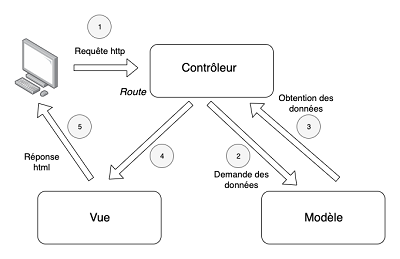
\includegraphics[width=15cm, height=8cm]{./Template LaTeX/Images/Modèle-vue-contrôleur_(MVC)_-_fr.png}
	\caption{MVC}
	\label{fig:birds}
\end{figure}
\newline \newline \newline
\textbf{Les fichiers sont organisés comme suit :}
\begin{enumerate}
	\item [-] \textbf{Route (Dispatcher) : }il contient les définitions des chemins d’entrées pour l’utilisateur,
	autrement dit les URI possibles et les dirige sur la classe définit dans
	le contrôleur qui doit traiter l’information.
	\item [-] \textbf{ Modèle : }pour chaque table de notre base de données que l’on veut
	utiliser pour notre application, il faut créer un modèle pour chacun.
	Ainsi nous avons ici un modèle de notre application. Il permet de
	décrire la méthode d’accès aux données de la base, tous cela à
	travers un objet définit par ORM Eloquent(Object-Relational
	Mapping).
	\item [-] \textbf{Contrôleur : } il permet de récupérer les informations du modèle et de l’envoyer
	vers la vue pour la mise en forme.
	\item [-] \textbf{Vue : } la vue réceptionne la réponse qui est envoyée par le
	contrôleur .\newline
\end{enumerate}







\section{Choix des outils de travail }
\subsection{Langages utilisés}
\subsubsection{Dart}
Dart est un langage de programmation open source à usage général. Il est initialement développé par Google. Dart est un langage orienté objet avec une syntaxe de C-style. Il prend en chargent les concepts de programmation tels que les interfaces, les classes, contrairement aux autres langages de programmation, Dart ne prend pas en charge les tableaux.
Les collections Dart peuvent être utilisées pour répliquer des structures de données telles que des tableaux, des génériques et un typage facultatif.
\newline Pour en savoir plus, veillez
visiter le lien : \href{https://www.tutorialspoint.com/flutter/flutter_introduction_to_dart_programming.htm}{https://www.tutorialspoint.com/flutter/dart}
\subsubsection{PHP}
PHP est un langage de script utilisé le plus souvent côté serveur : dans cette architecture, le serveur interprète le code PHP des pages web demandées et génère du code (HTML, XHTML, CSS par exemple) et des données (JPEG, GIF, PNG par exemple) pouvant être interprétés et rendus par un navigateur web. PHP peut également générer d'autres formats comme le WML, le SVG et le PDF.

Il a été conçu pour permettre la création d'applications dynamiques, le plus souvent développées pour le Web. PHP est le plus souvent couplé à un serveur Apache bien qu'il puisse être installé sur la plupart des serveurs HTTP tels que IIS ou nginx. Ce couplage permet de récupérer des informations issues d'une base de données, d'un système de fichiers (contenu de fichiers et de l'arborescence) ou plus simplement des données envoyées par le navigateur afin d'être interprétées ou stockées pour une utilisation ultérieure.
\newline Pour en savoir plus, veillez
visiter le lien : \href{https://fr.wikipedia.org/wiki/PHP}{https://fr.wikipedia.org/wiki/PHP}
\subsection{Frameworks utilisés}

\subsubsection{Flutter}
Flutter est un framework de développement d’applications mobiles open source de Google. La principale raison de sa popularité est qu’il prend en charge la création 		   
d’applications multiplateformes. Flutter est également utilisé pour créer des apps interactives qui s’exécutent sur des pages web ou sur le bureau.\newline
\textbf {- Les caractéristiques de Flutter :}


\begin{enumerate}
	\item Base de code unique pour Android et iOS
	\item Fonction de rechargement à chaud (hot reload)
	\item Open-source et par Google
	\item Programmation Dart \newline \newline \newline
\end{enumerate}
\newpage

\textbf {- Architecture d’une application Flutter :} \newline \newline \newline
\begin{figure}[h!]
	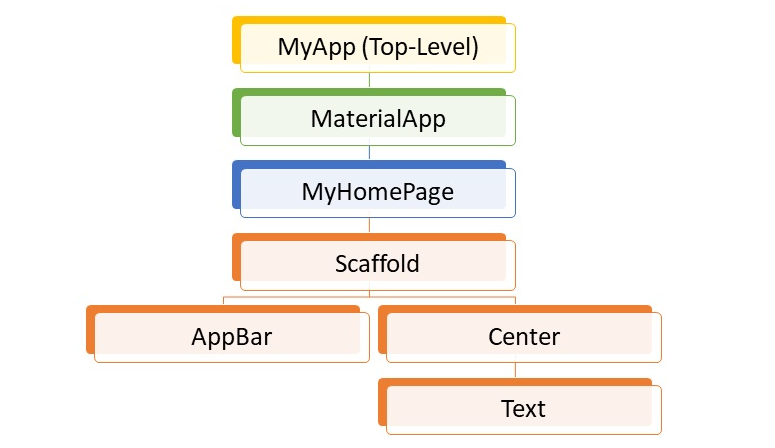
\includegraphics[width=400px,height=200px]{./Template LaTeX/Images/Flutter_architect.png}
	\caption{Architecture d’une application Flutter.}
	\label{fig:birds}
\end{figure}
\subsubsection{Laravel}
Laravel est un framework web open-source écrit en  \href{https://fr.wikipedia.org/wiki/PHP}{PHP} respectant le principe modèle-vue-contrôleur et entièrement développé en programmation orientée objet. Laravel est distribué sous \href{https://fr.wikipedia.org/wiki/Licence_MIT}{licence MIT}, avec ses sources hébergées sur 
\href{https://fr.wikipedia.org/wiki/GitHub}{GitHub}.

\section{Implémentation}
\subsection{Etape de réalisation}
Pour réaliser notre système, il y a des étapes à élaborer dans l’ordre suivant :
\begin{itemize}[label=$\ast$]
	\item \textbf{Conception de la base de données :} La conception d’une base de données est la
	première étape. Le choix des algorithmes et de l’approche de travail exige l’utilisation
	d’une base de données spécifique (en fonction du système à développer).
	\item \textbf{Extraction des données :}  On va utiliser notre SGBD Firebase ainsi que notre base de
	données en interaction avec l’application pour extraire des informations. Firebase est
	conçu avec des fonctionnalités et des requêtes de sélection de données assez spécifique
	et facile à utiliser.
	\item \textbf{Conception et développement du front-end et du back-end :} 
	Cette étape consiste à
	détailler la conception coté client et coté serveur. Il s’agit de mettre en place un design
	ergonomique, simple et attractif répondant aux exigences du système. Le choix d’un
	serveur d’application adéquat aux fonctionnalités et aux données est une étape
	fondamentale pour le bon fonctionnement de l’application.
	\item \textbf{Développement de back-end :} On commence par le développement de l’application coté
	serveur, dans notre cas avec \textbf{Laravel}. C’est la partie du code exécuté sur le serveur afin
	de vérifier le comportement des fonctionnalités de base du système.
	\item \textbf{Développement front-end :} On développe la partie client en interaction avec le serveur.
	C’est la conception de l'interface graphique utilisateur. En effet, il s'agit de la partie
	visible de l'application, destinée à être manipulée par un tiers.
\end{itemize}
\subsection{Interfaces Homme/Machine}
Dans ce qui suit, nous présentons quelques écrans de notre produit final des applictions CADORIM et Cadorim service.
\subsubsection{Application CADORIM}
\begin{itemize}[label=$\ast$]
		\item \textbf{Première interface :} L'utilisateur du Cadorim avant d'être invite à consulter les services de l'application, doit 
			choisies leur langue avant qu'il pass a l'interface suivante.
			
			\begin{figure}[!ht]
				\centering
				\begin{subfigure}{0.3\textwidth}
					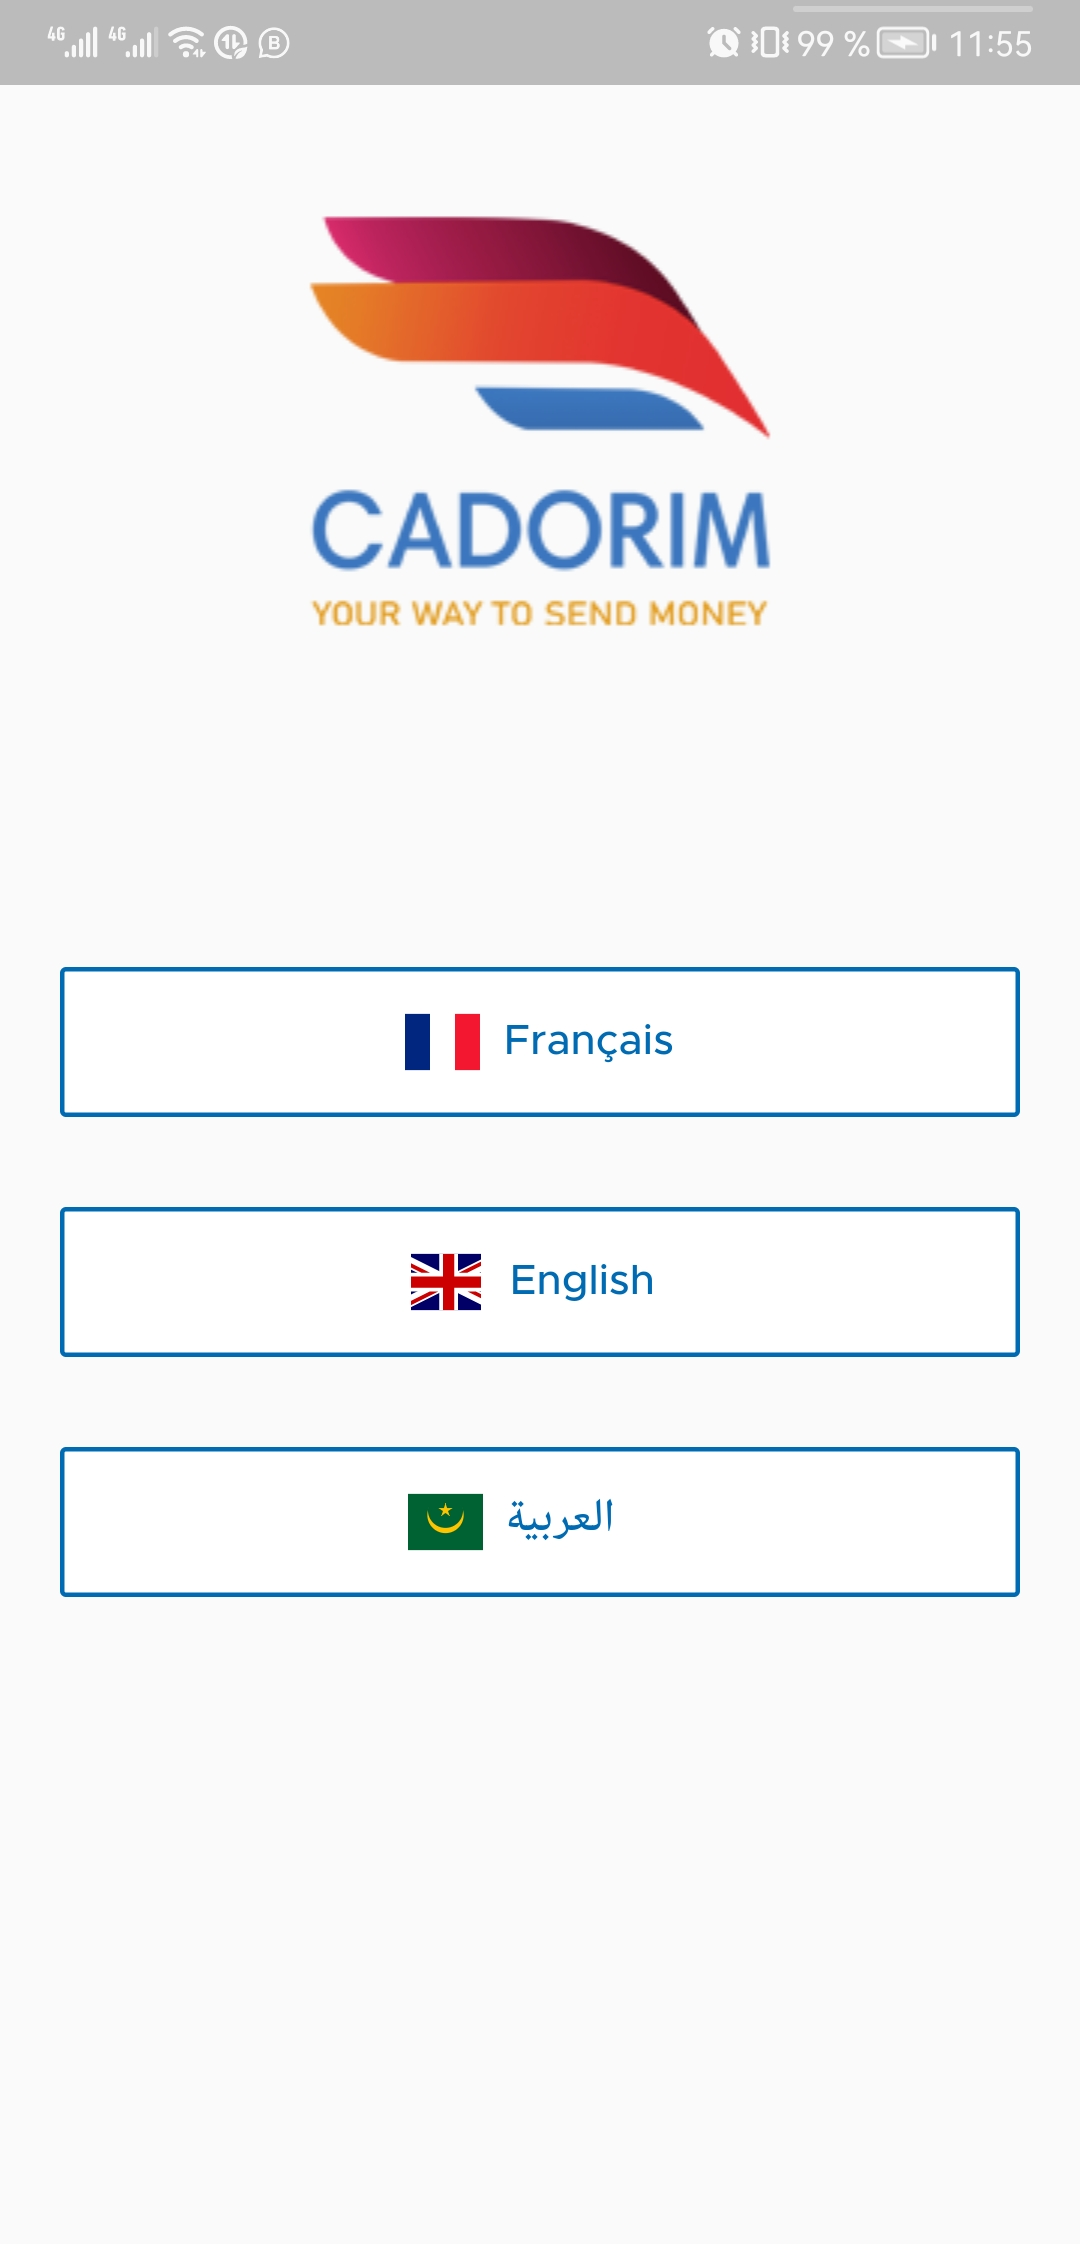
\includegraphics[width=\hsize, valign=m ]{./Template LaTeX/Images/1.jpg}
					\caption{Choix de langue}
					\label{fig.SICAPI}
				\end{subfigure}
				\qquad\tikz[baseline=-\baselineskip]\draw[ultra thick,->] (0,0) -- ++ (1,0);\qquad
				\begin{subfigure}{0.3\textwidth}
					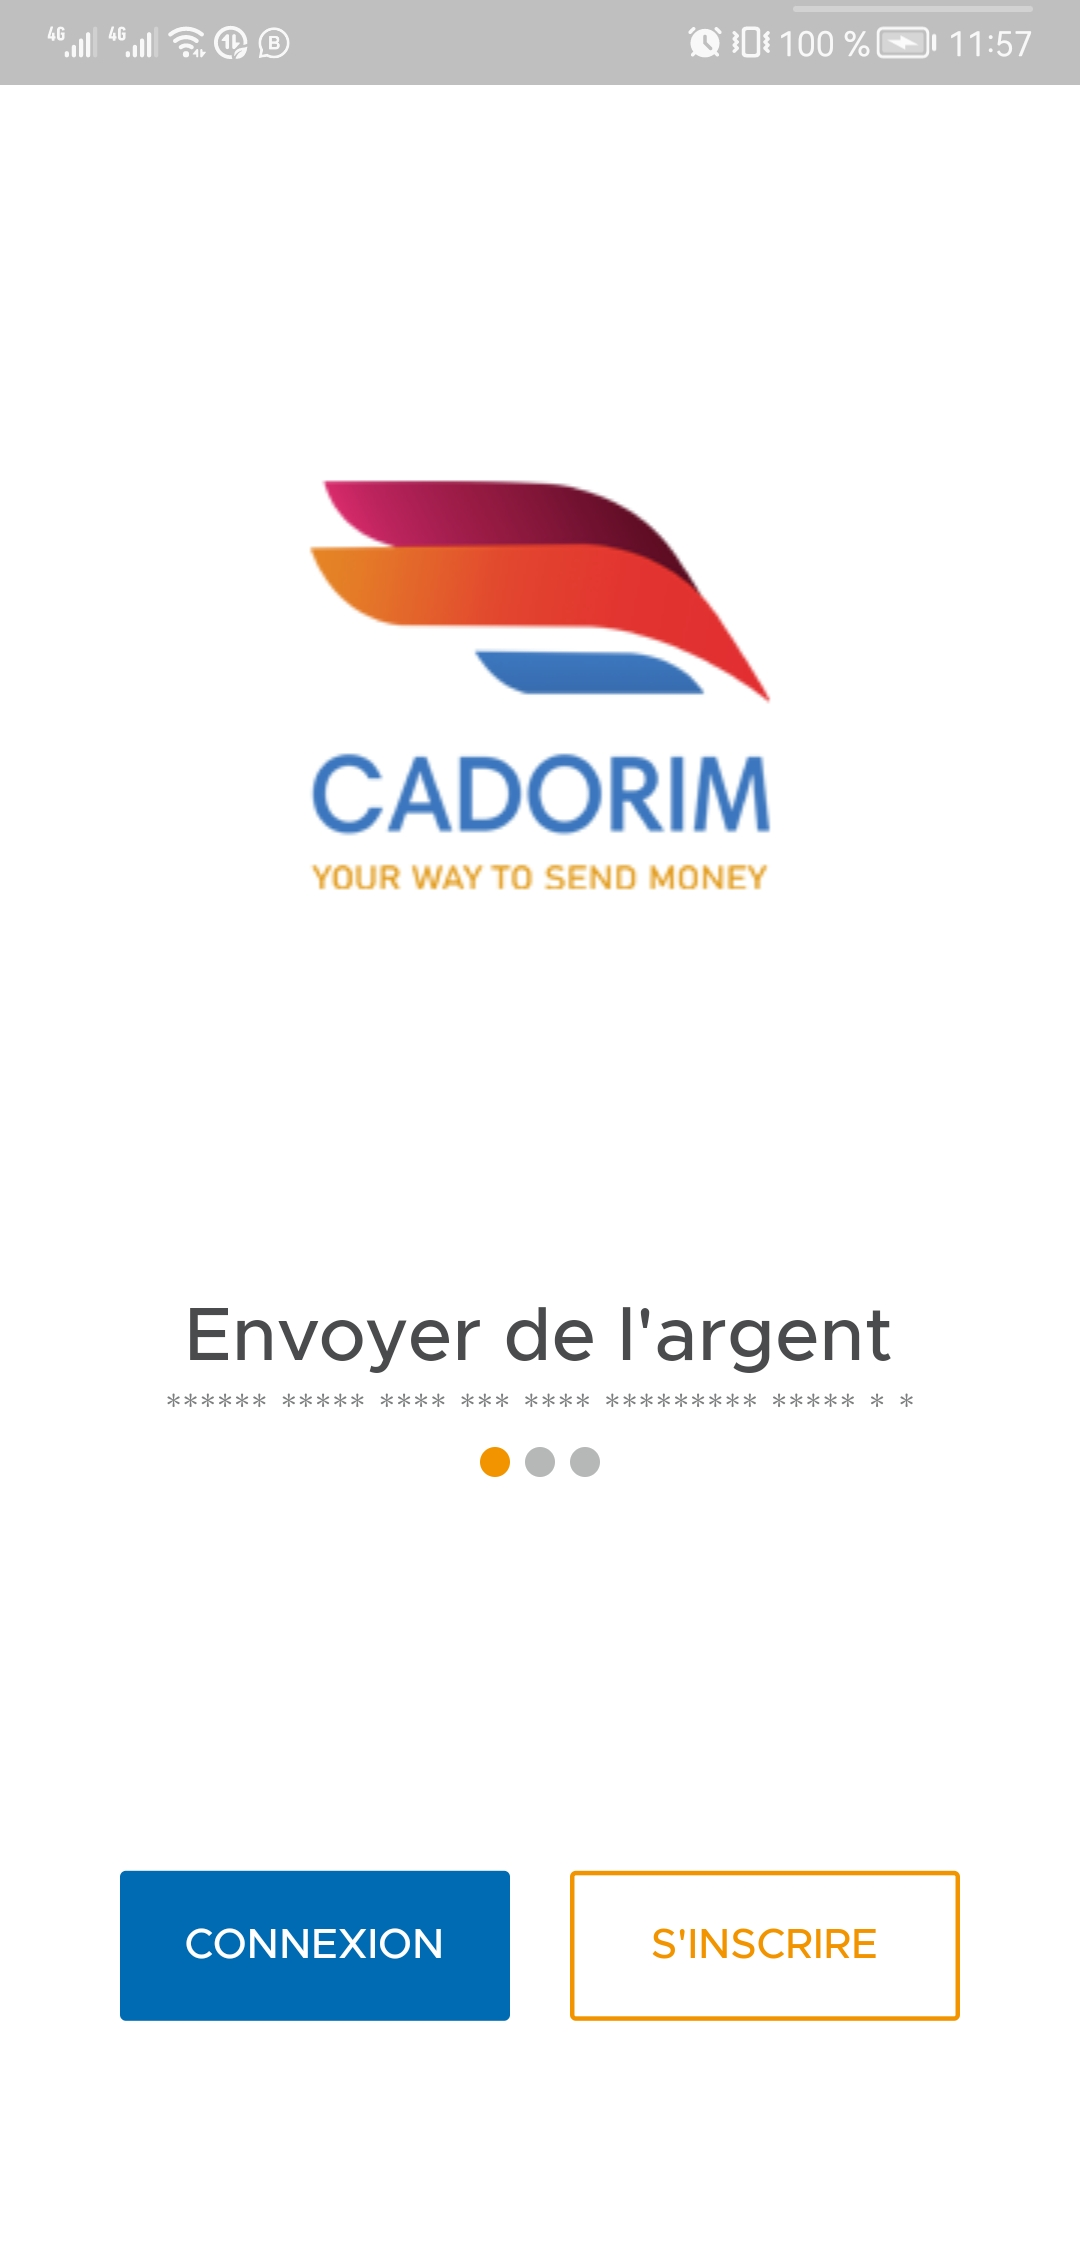
\includegraphics[width=\hsize, valign=m]{./Template LaTeX/Images/2.jpg}
					\caption{Interface suivante}
					\label{fig.painel_sicapi}
				\end{subfigure}
				\caption{Première interface}
				\label{fig.sicapi}
			\end{figure}
		%%%%%%%%%%%%%%%%%%%%%%%%%%%%%%% authentificationb %%%%%%%%%%%%
		\newpage
		\item \textbf{L’interface
			d’authentification
			:} La figure suivante représente l’interface d’authentification de notre application. Elle permet aux utilisateurs de s’identifier en introduisant leurs identifiants afin d’accéder aux fonctionnalités de l’application.
			\begin{figure}%
				\centering
				{{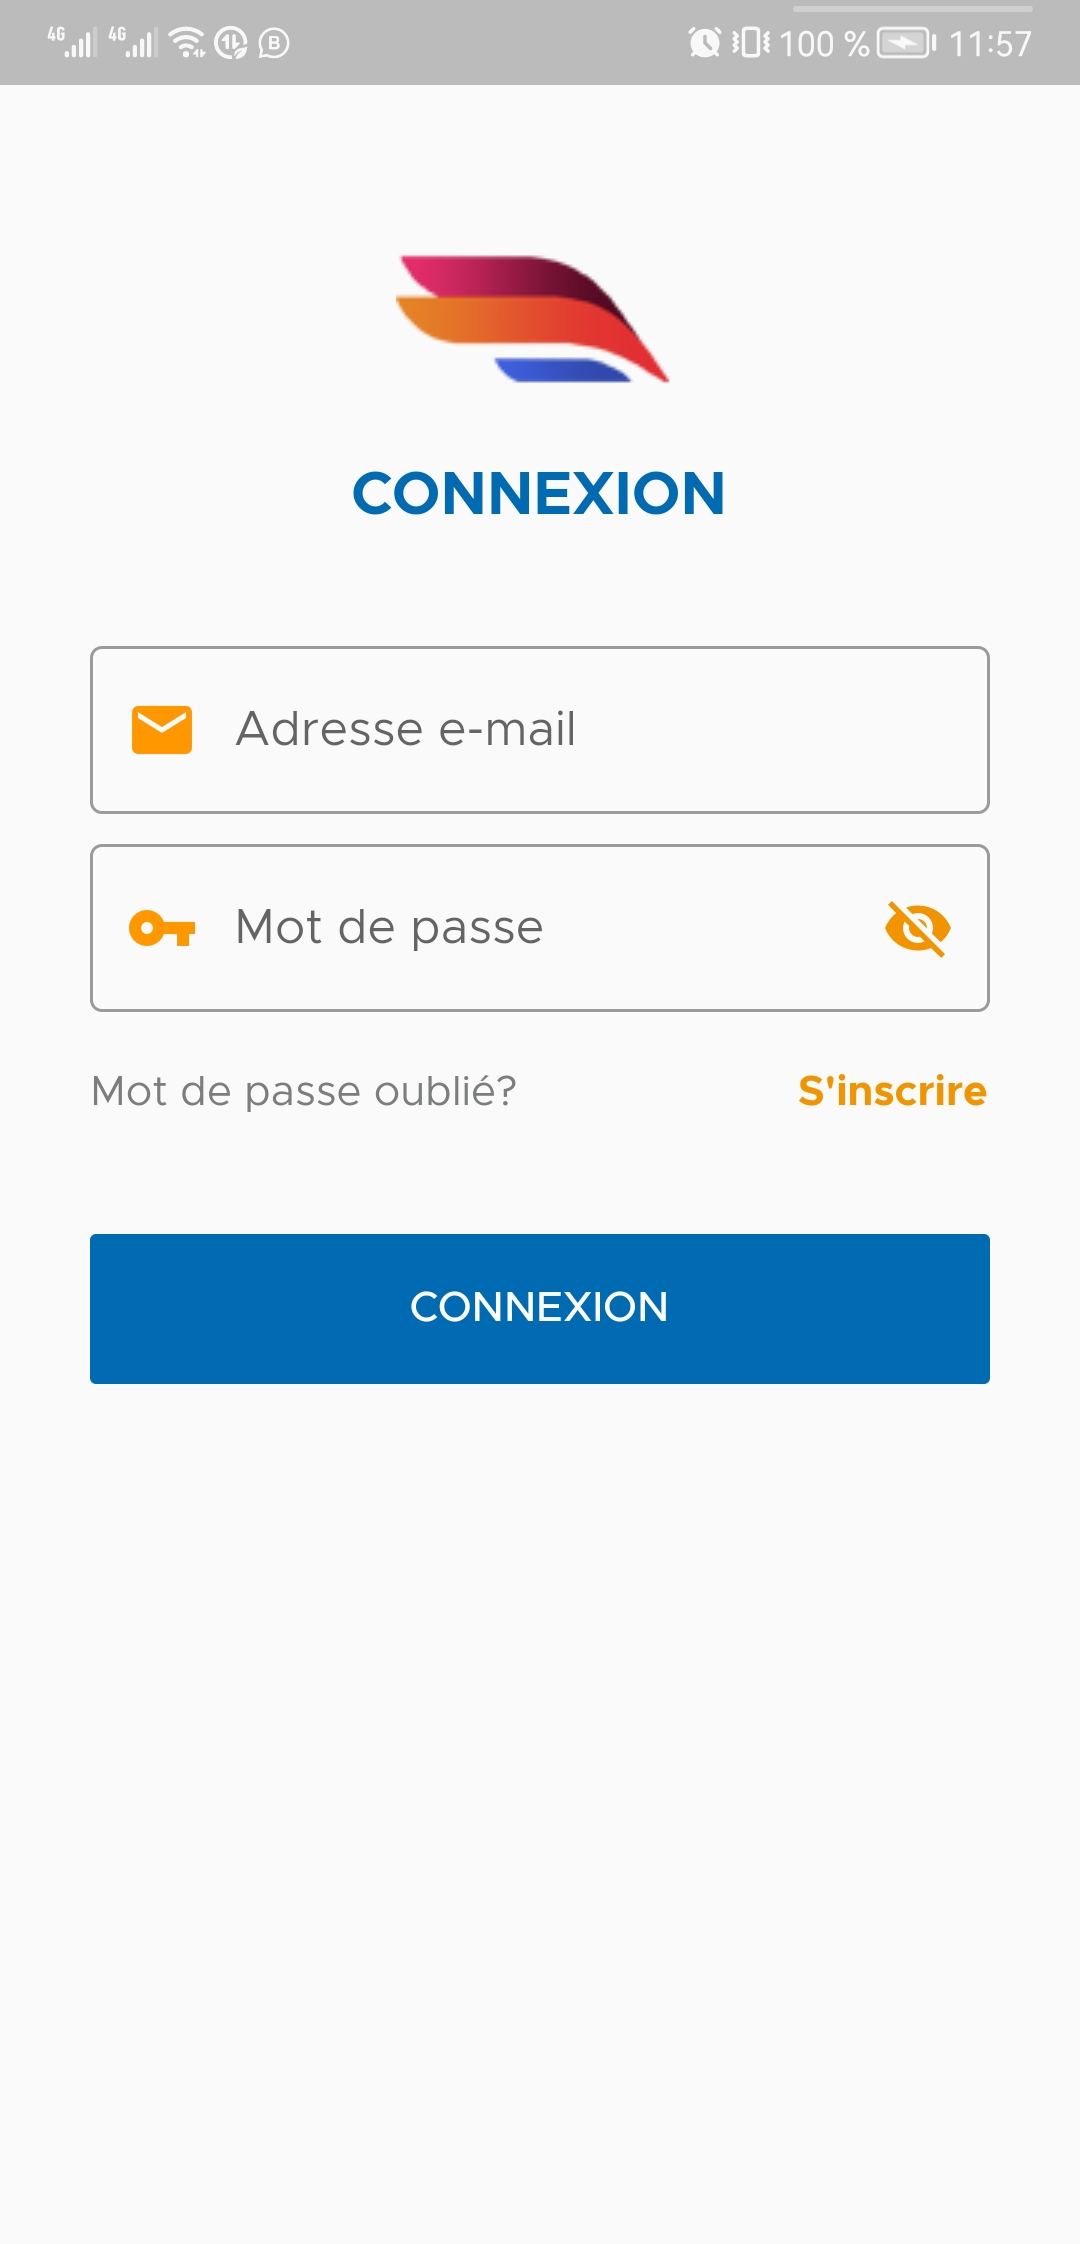
\includegraphics[width=5cm]{./Template LaTeX/Images/3.jpg} }}%
				\caption{Interface d'authentification}%
				\label{fig:example}%
			\end{figure}
		\newpage
		La demande d’identification du client est traitée pour vérifier ses paramètres dans la base de
		données. L’absence de l’utilisateur dans la base de données ou une erreur de saisie des
		informations entraine une alerte d’erreur d’authentification.
		%%%%%%%%%%%%%%%%%%%%%%%%%% Inscruire %%%%%%%%%%%%%%%%%%%%%%5
		\item \textbf{L’interface d’inscription :}
		Avant de pouvoir s’authentifier, l’utilisateur doit
		impérativement s’enregistrer au préalable dans la base de données. La figure suivante
		représente l’interface de création de compte pour un client.
		\begin{figure}[!ht]
			\centering
			\begin{subfigure}{0.3\textwidth}
				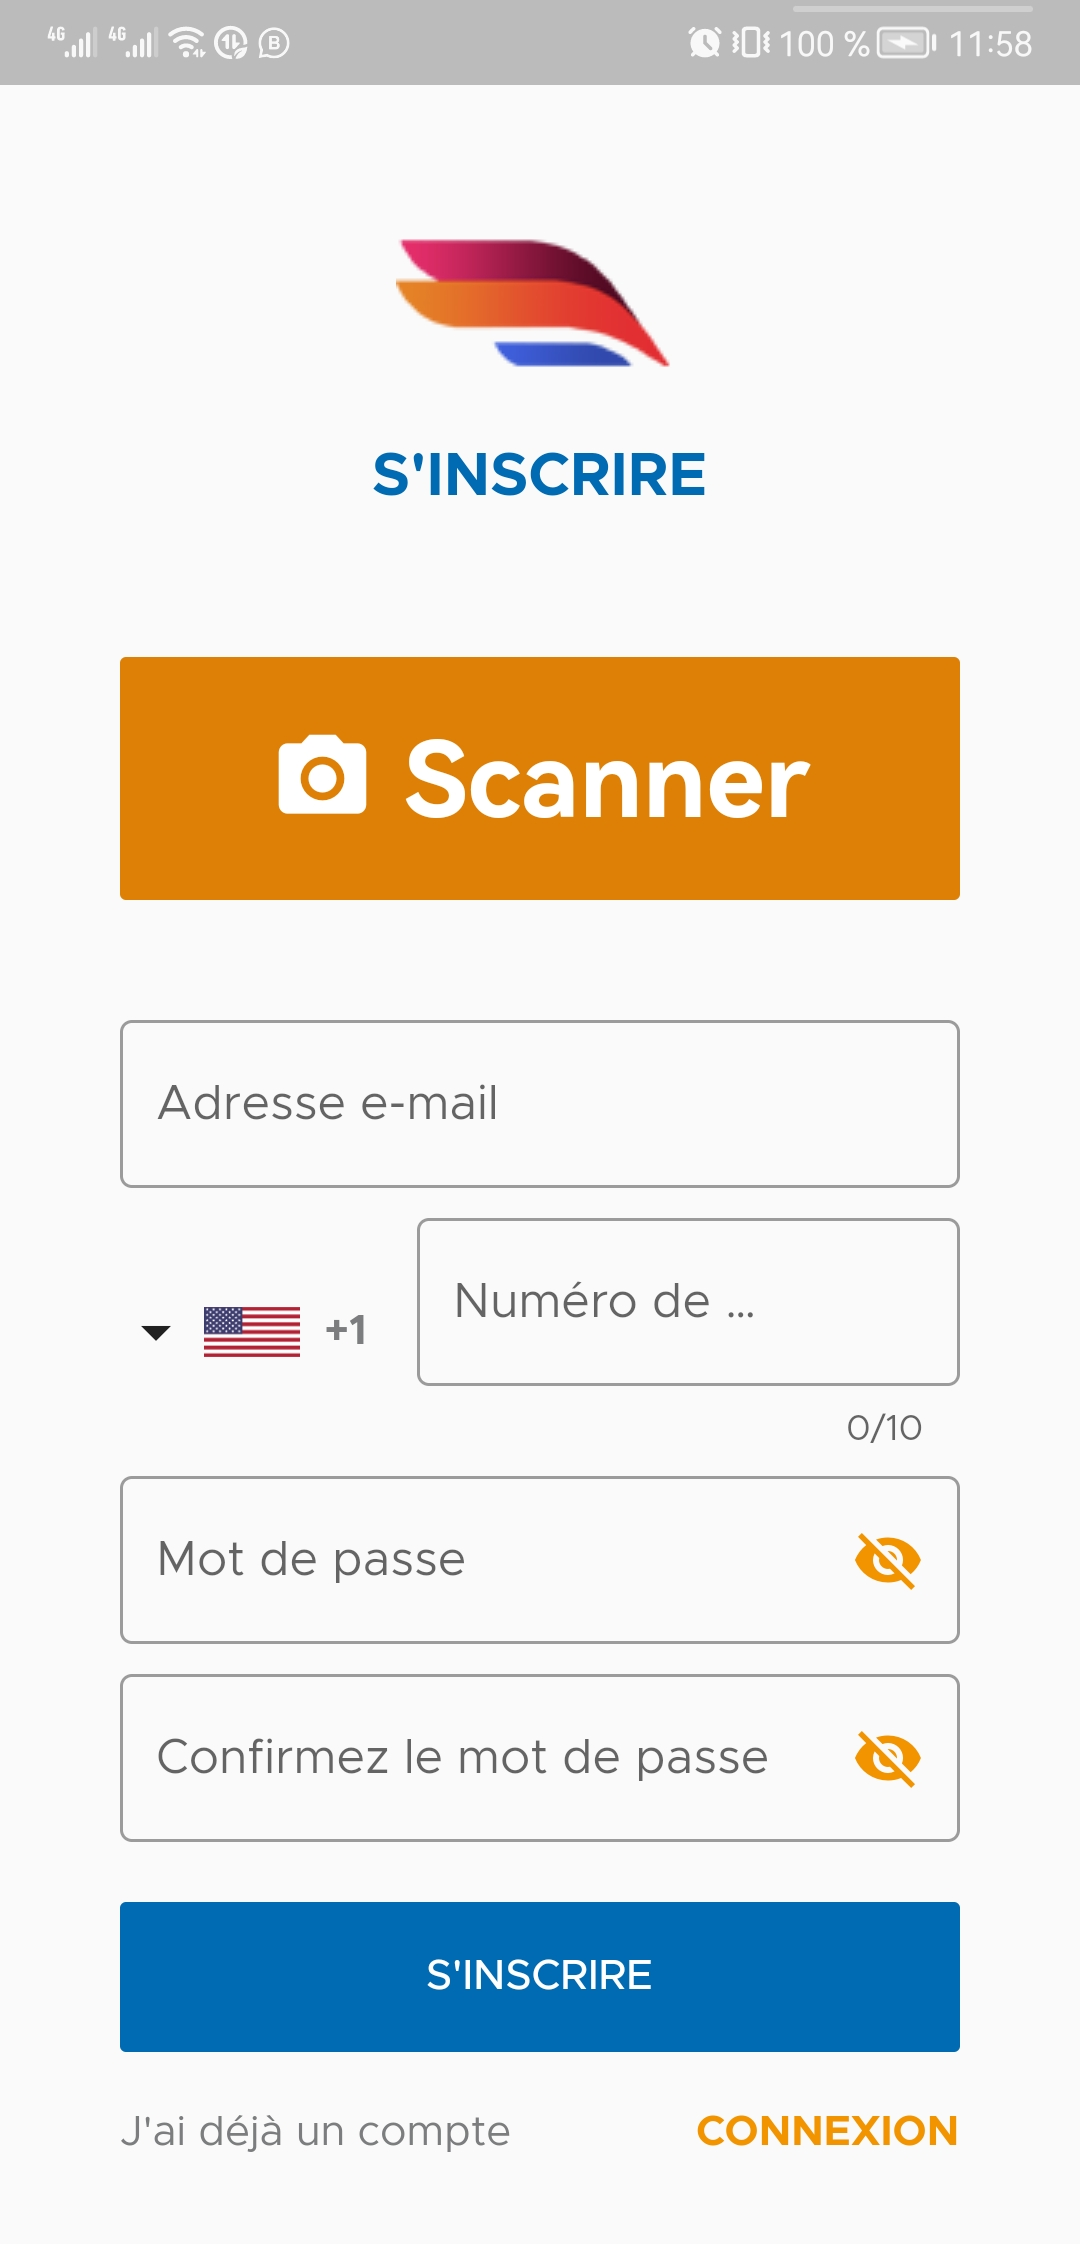
\includegraphics[width=\hsize, valign=m ]{./Template LaTeX/Images/4.jpg}
				\caption{Interface d’inscription}
				\label{fig.SICAPI}
			\end{subfigure}
			\qquad\tikz[baseline=-\baselineskip]\draw[ultra thick,->] (0,0) -- ++ (1,0);\qquad
			\begin{subfigure}{0.3\textwidth}
				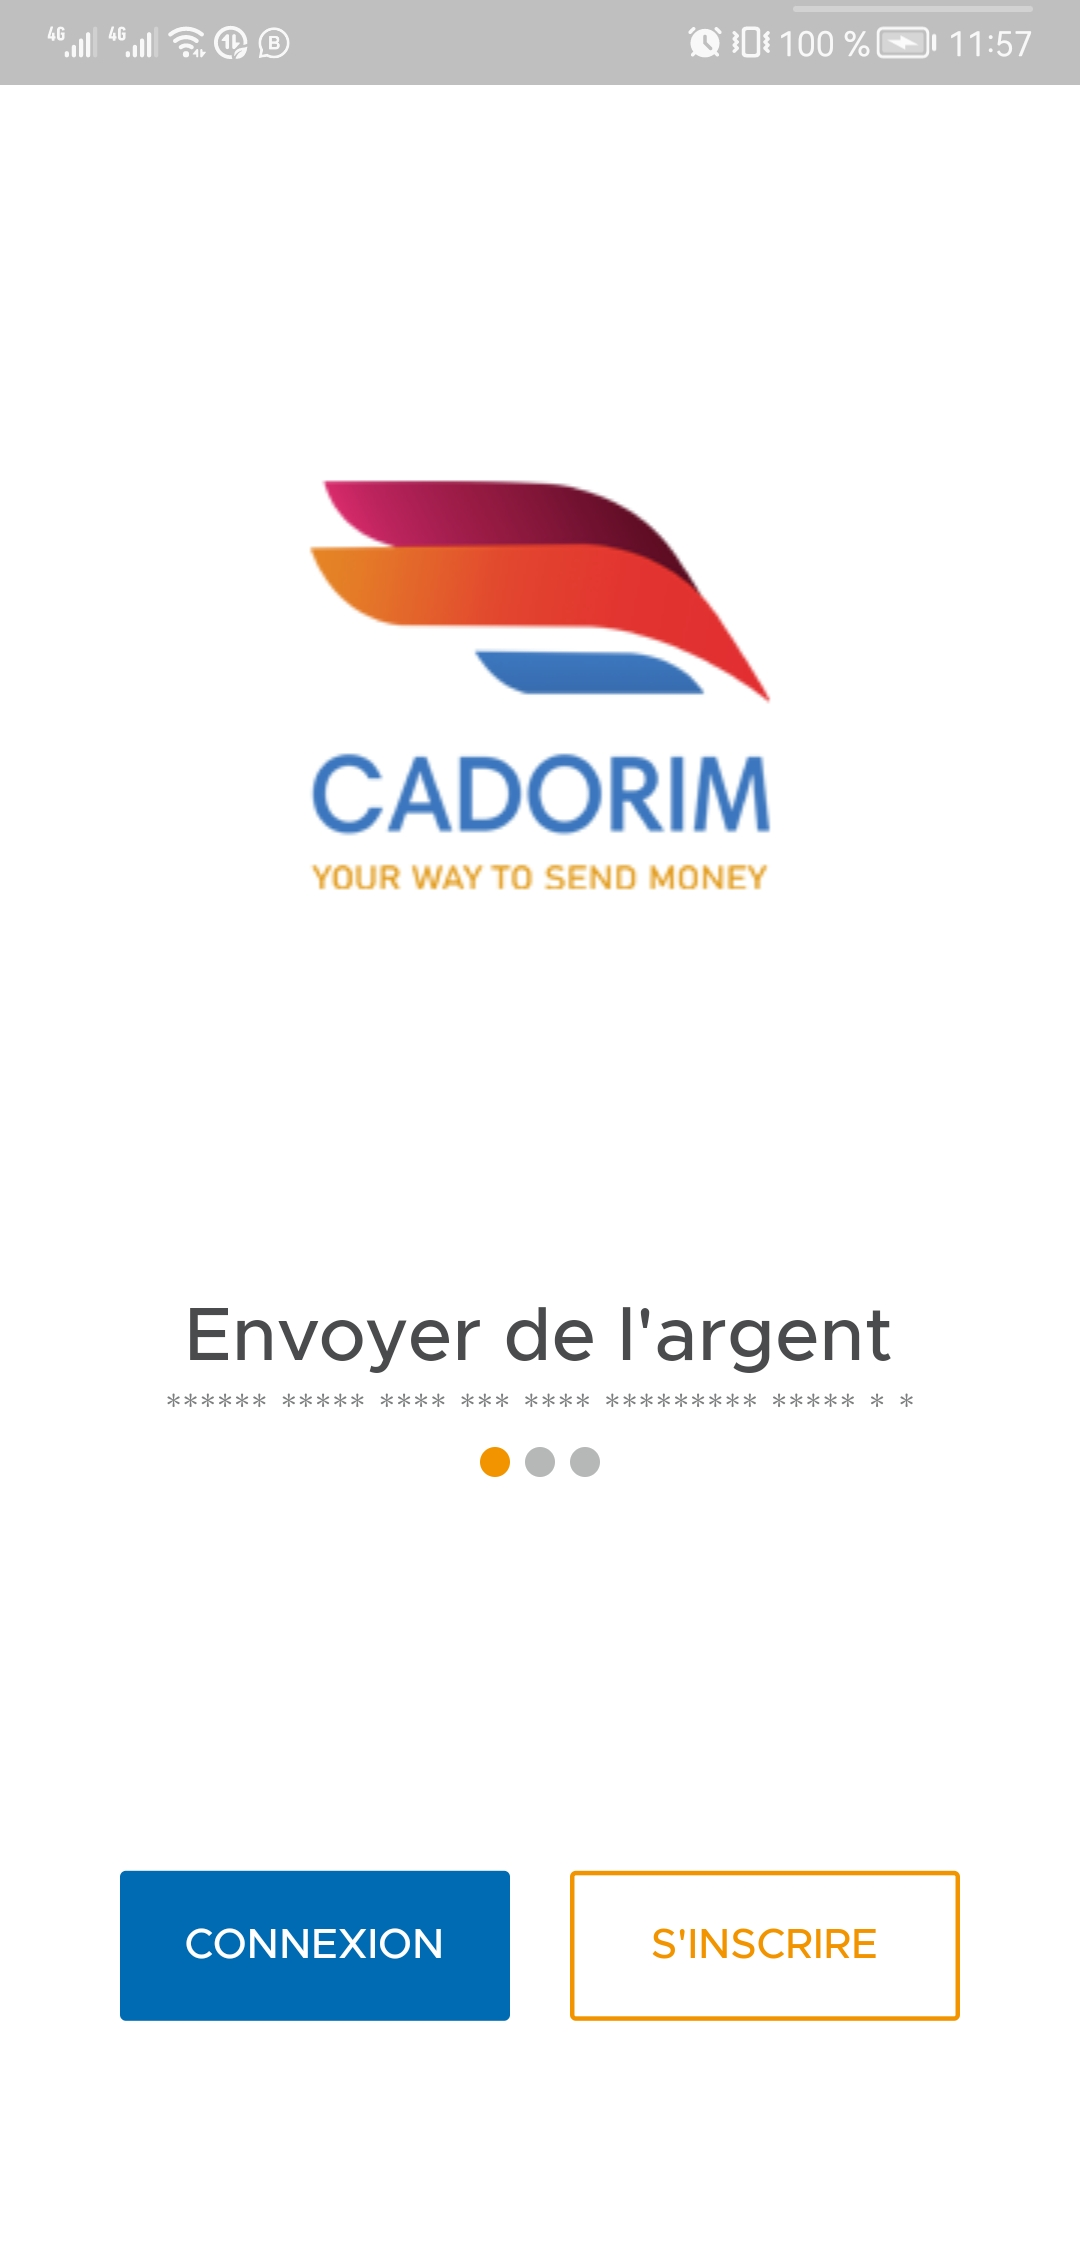
\includegraphics[width=\hsize, valign=m]{./Template LaTeX/Images/2.jpg}
				\caption{Scanner le code MRZ}
				\label{fig.painel_sicapi}
			\end{subfigure}
			\caption{Interface d’inscription}
			\label{fig.sicapi}
		\end{figure}
	
	%%%%%%%%%%%%%%%%%%%%%%%%%%%%%5 Home
	
	%%%%%%%%%%%%%%%%%%%%%%%%%%%%%%%%%%%%
	\newpage
	\item \textbf{Processus de la transaction
		:} La figure suivante montre les processus de la transaction depuis la sélection de montant jusqu'à la validation (une notification de succès va Apparence si le traitement se fait avec succès)
\begin{comment}
	content...

\begin{figure}[!ht]
	\centering
	\begin{subfigure}{0.3\textwidth}
		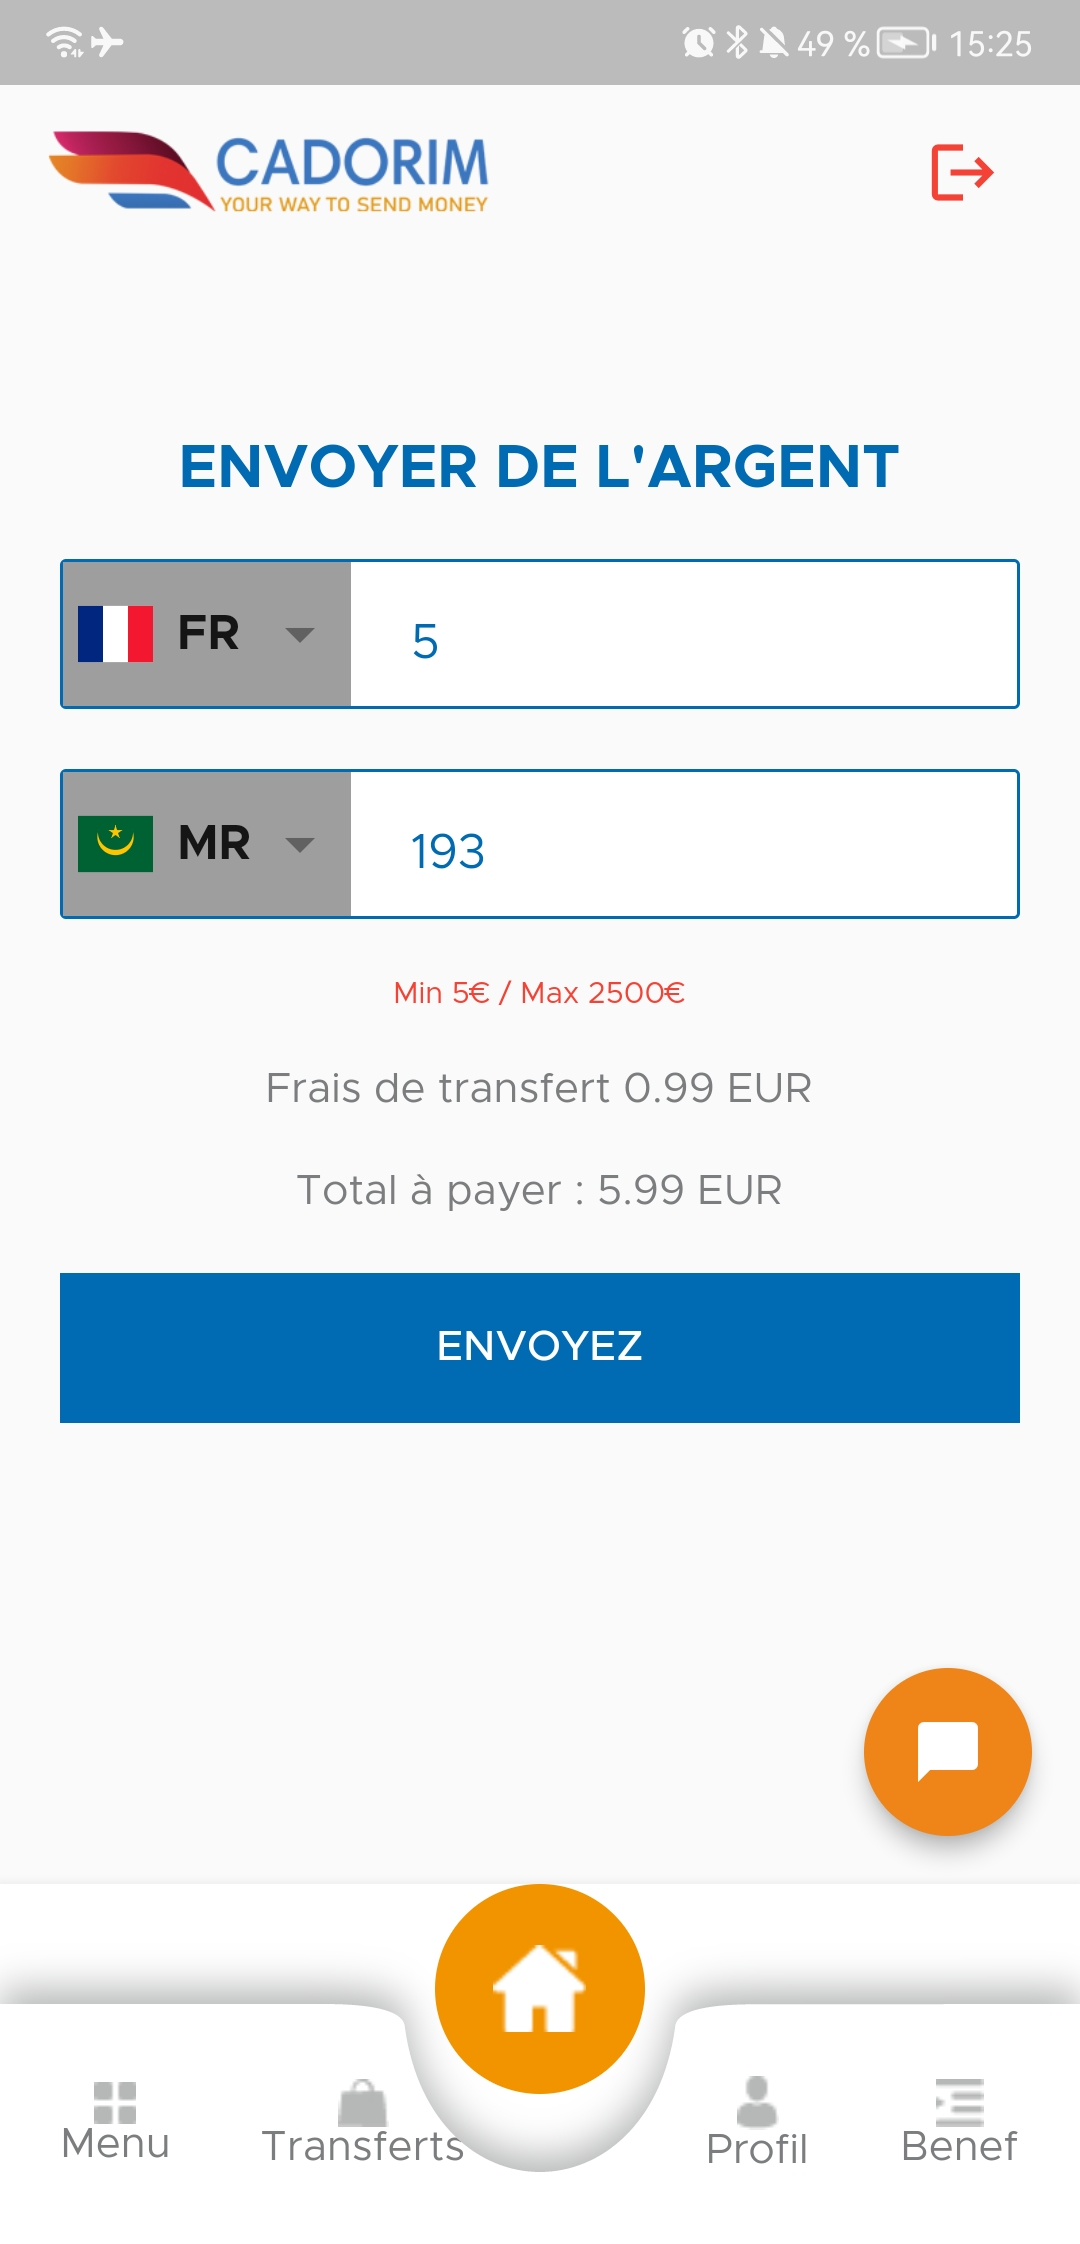
\includegraphics[width=\hsize, valign=m ]{./Template LaTeX/Images/5.jpg}
		\caption{Interfaces d'accueil}
		\label{fig.SICAPI}
	\end{subfigure}
	\qquad\tikz[baseline=-\baselineskip]\draw[ultra thick,->] (0,0) -- ++ (1,0);\qquad
	\begin{subfigure}{0.3\textwidth}
		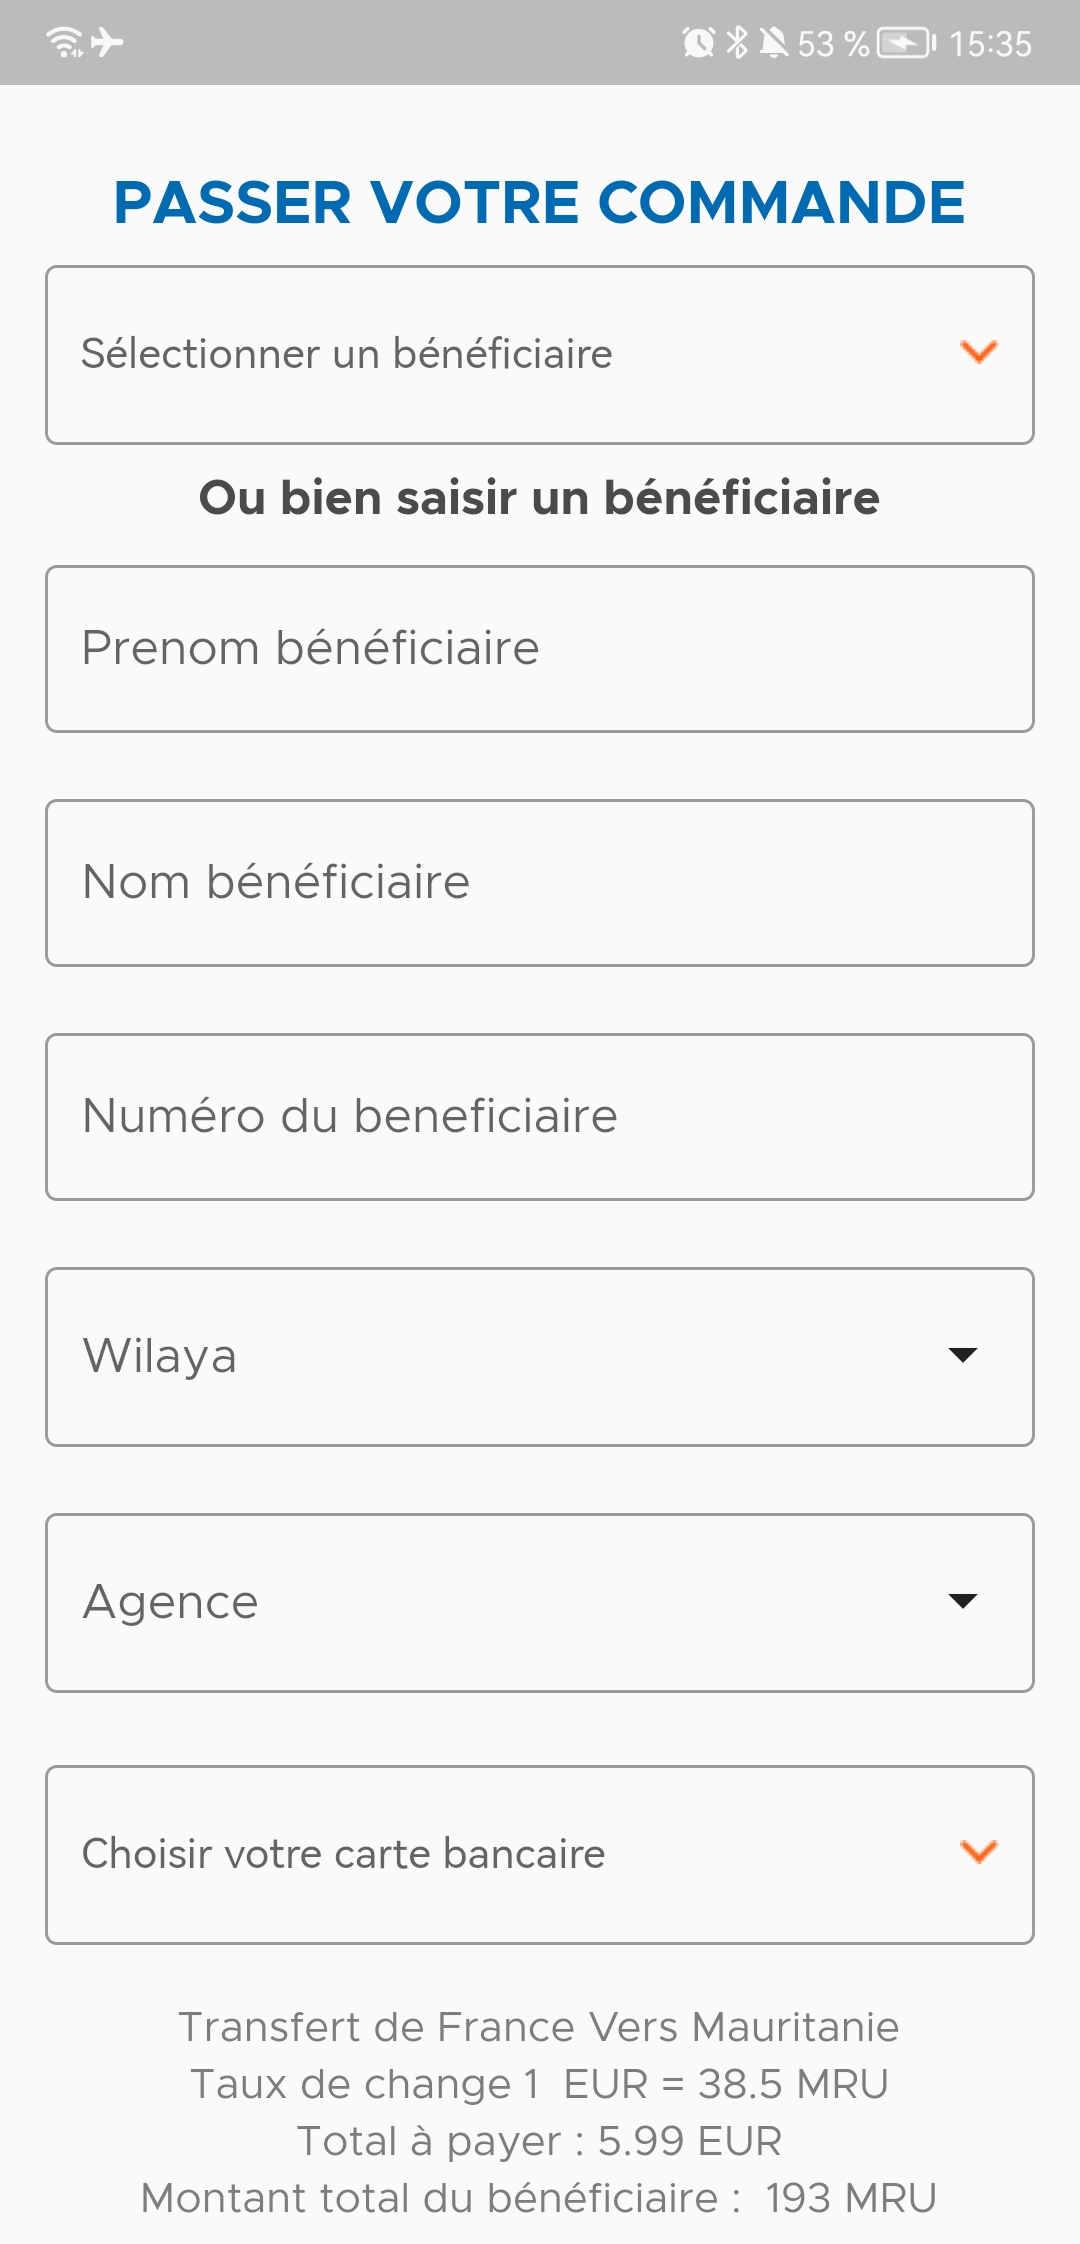
\includegraphics[width=\hsize, valign=m]{./Template LaTeX/Images/11.jpg}
		\caption{Interface de transfert}
		\label{fig.painel_sicapi}
	\end{subfigure}
%%%%%%%%%%%%%%%%%%%%%%%%%%%%%
\begin{subfigure}{0.3\textwidth}
	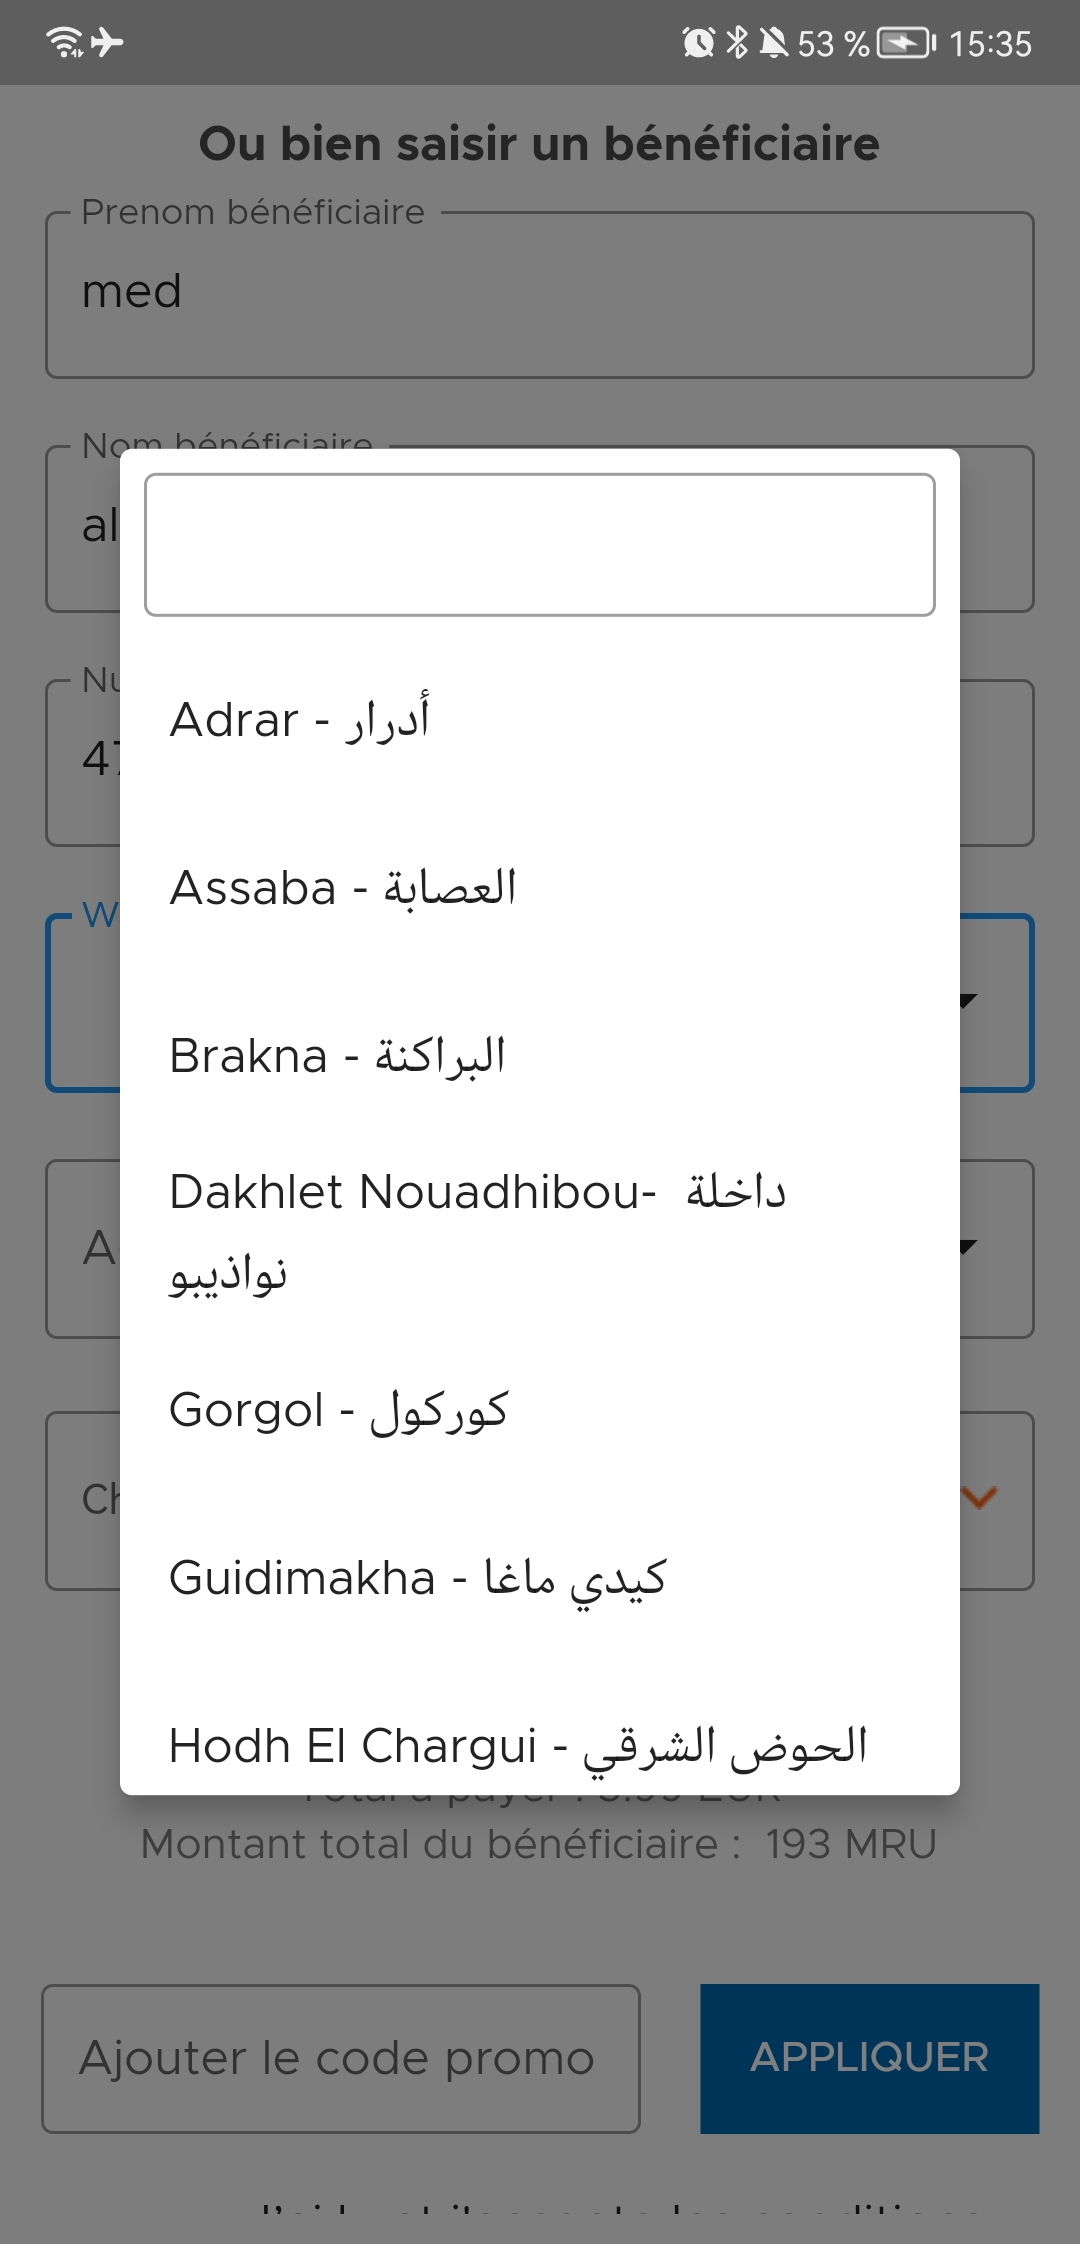
\includegraphics[width=\hsize, valign=m ]{./Template LaTeX/Images/12.jpg}
	\caption{Choix de wilaya}
	\label{fig.SICAPI}
\end{subfigure}
\qquad\tikz[baseline=-\baselineskip]\draw[ultra thick,->] (0,0) -- ++ (1,0);\qquad
\begin{subfigure}{0.3\textwidth}
	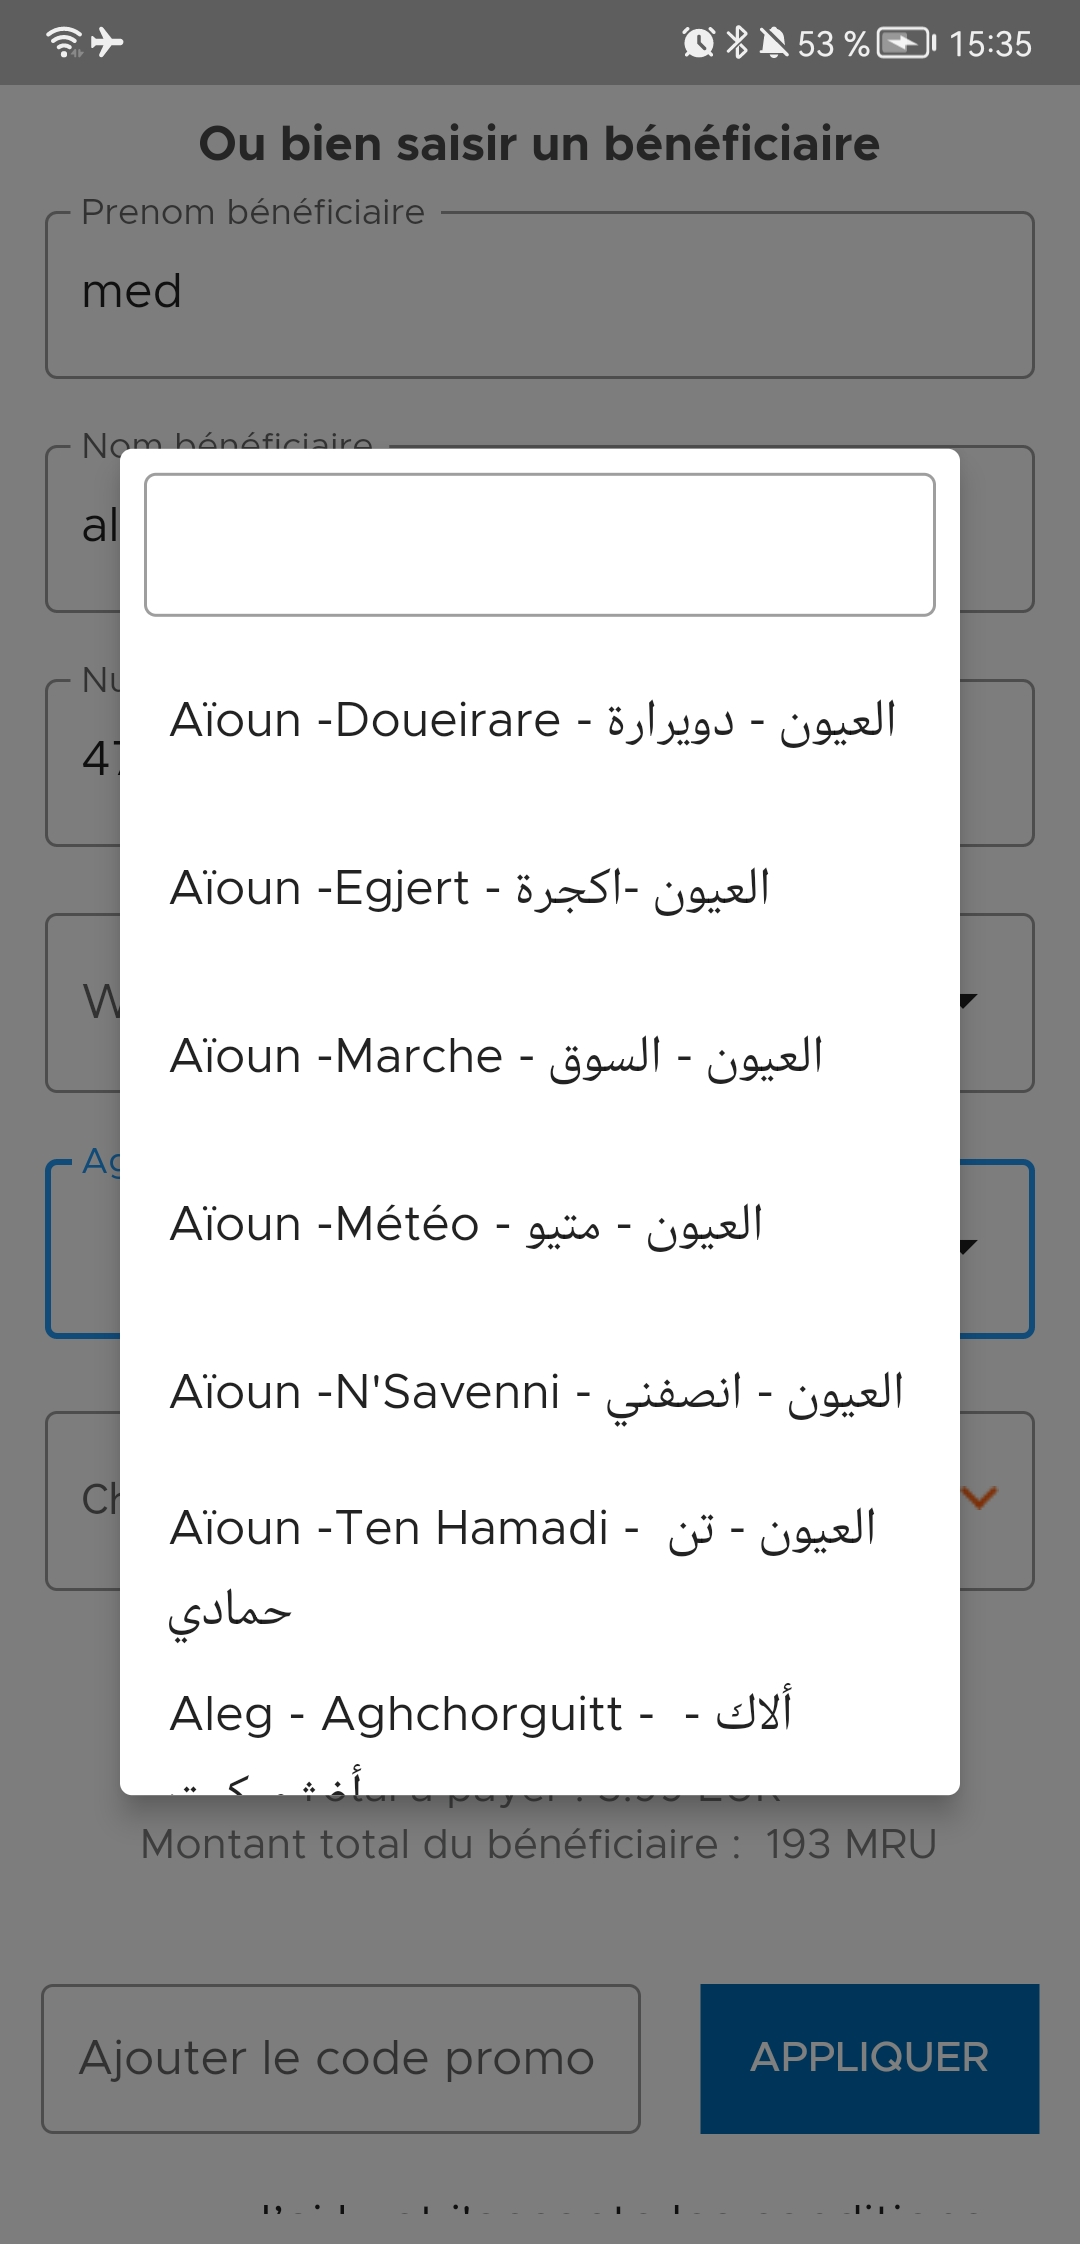
\includegraphics[width=\hsize, valign=m]{./Template LaTeX/Images/13.jpg}
	\caption{Choix d'agence}
	\label{fig.painel_sicapi}
\end{subfigure}
%%%%%%%%%%%%%%%%%%%%%%%%%%%%%%%%%%%%%%%%%%%%%%%%%%%%%%%%%%%

	\caption{Interfaces d'accueil}
	\label{fig.sicapi}
\end{figure}
\end{comment}
\begin{figure}
	\centering
	\begin{subfigure}[b]{0.3\textwidth}
		\centering
		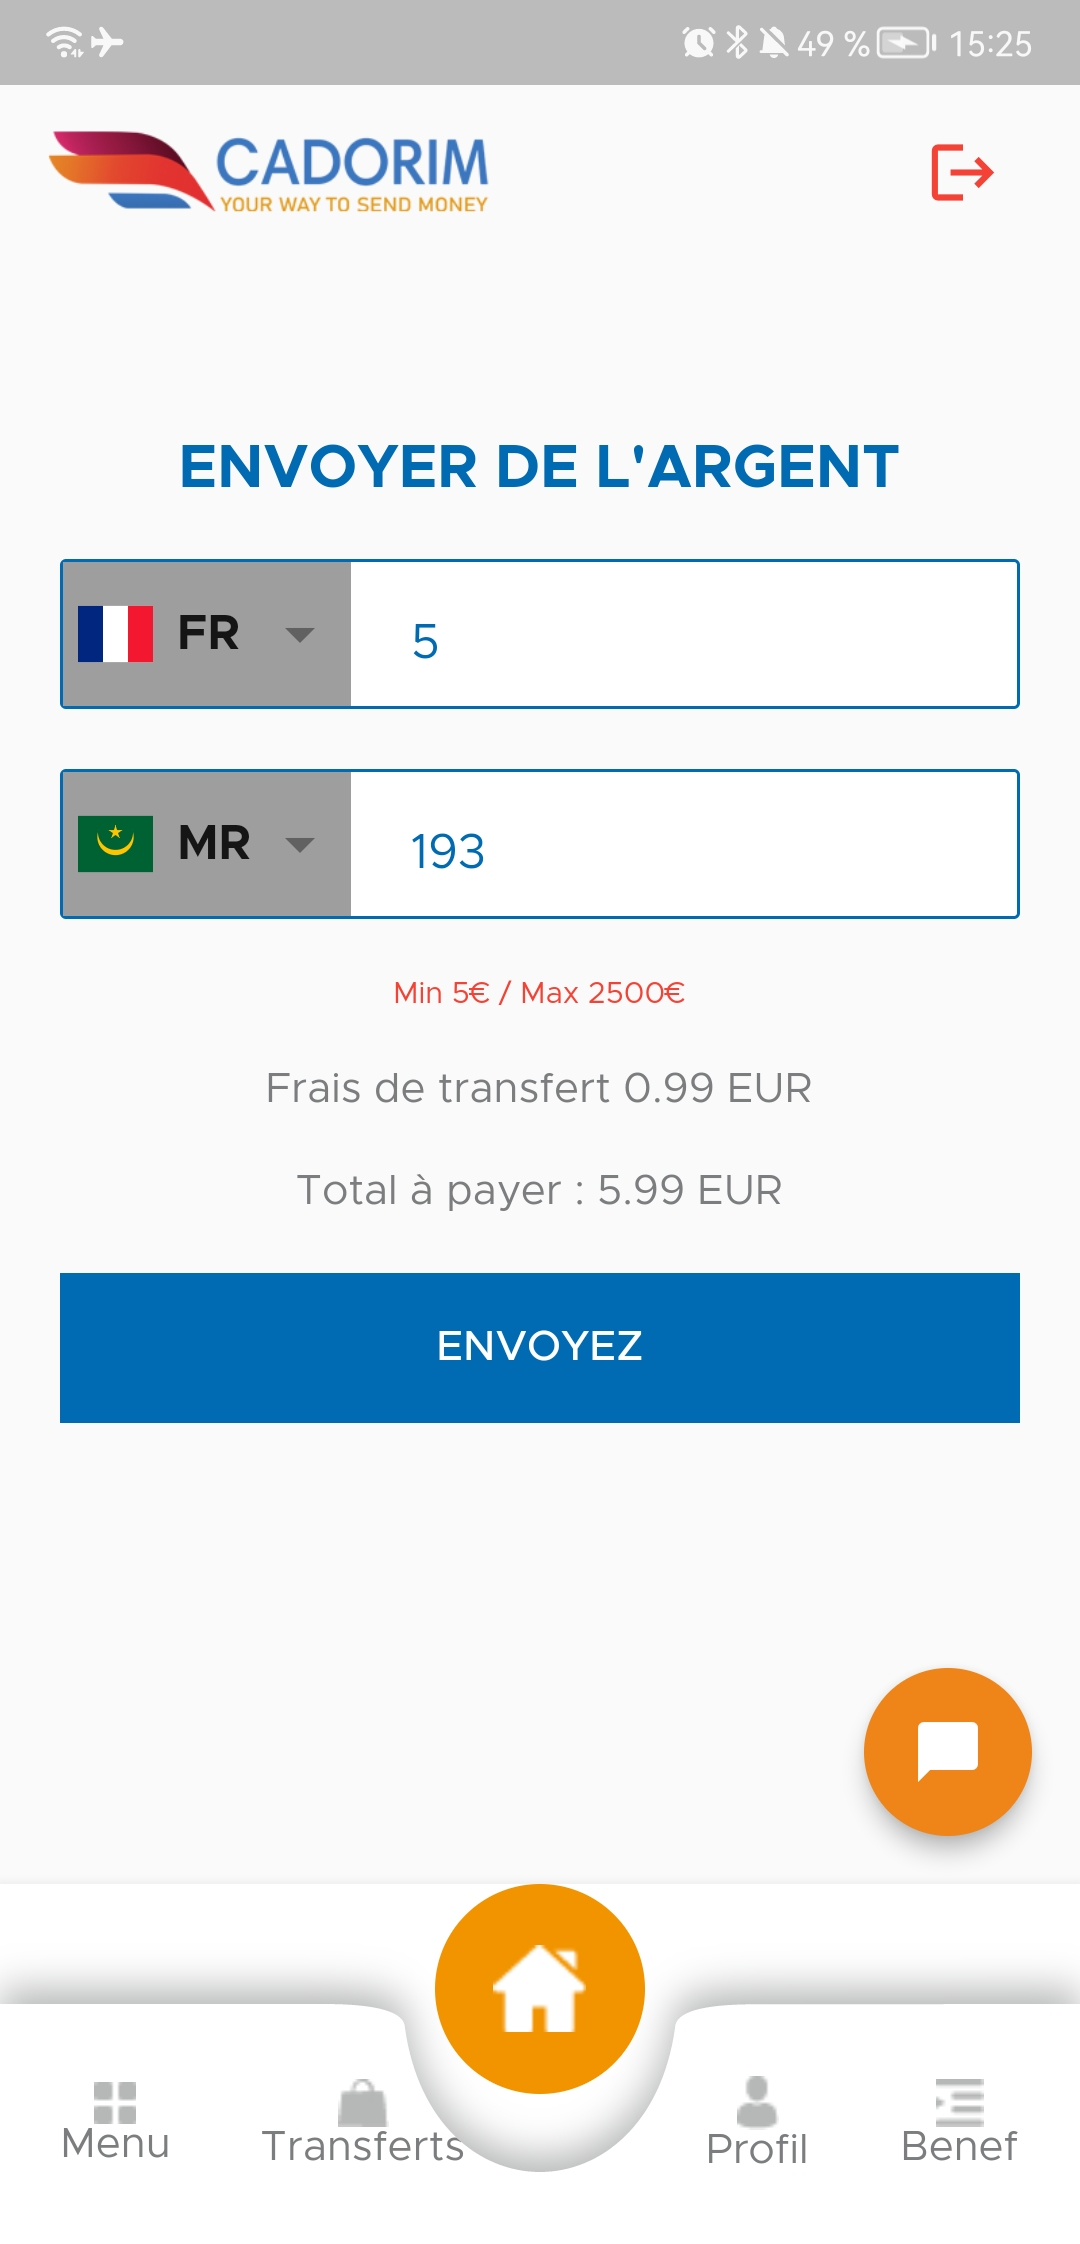
\includegraphics[width=\textwidth]{./Template LaTeX/Images/5.jpg}
		\caption{Interfaces d'accueil}
		\label{fig:y equals x}
	\end{subfigure}
	\hfill
	\begin{subfigure}[b]{0.3\textwidth}
		\centering
		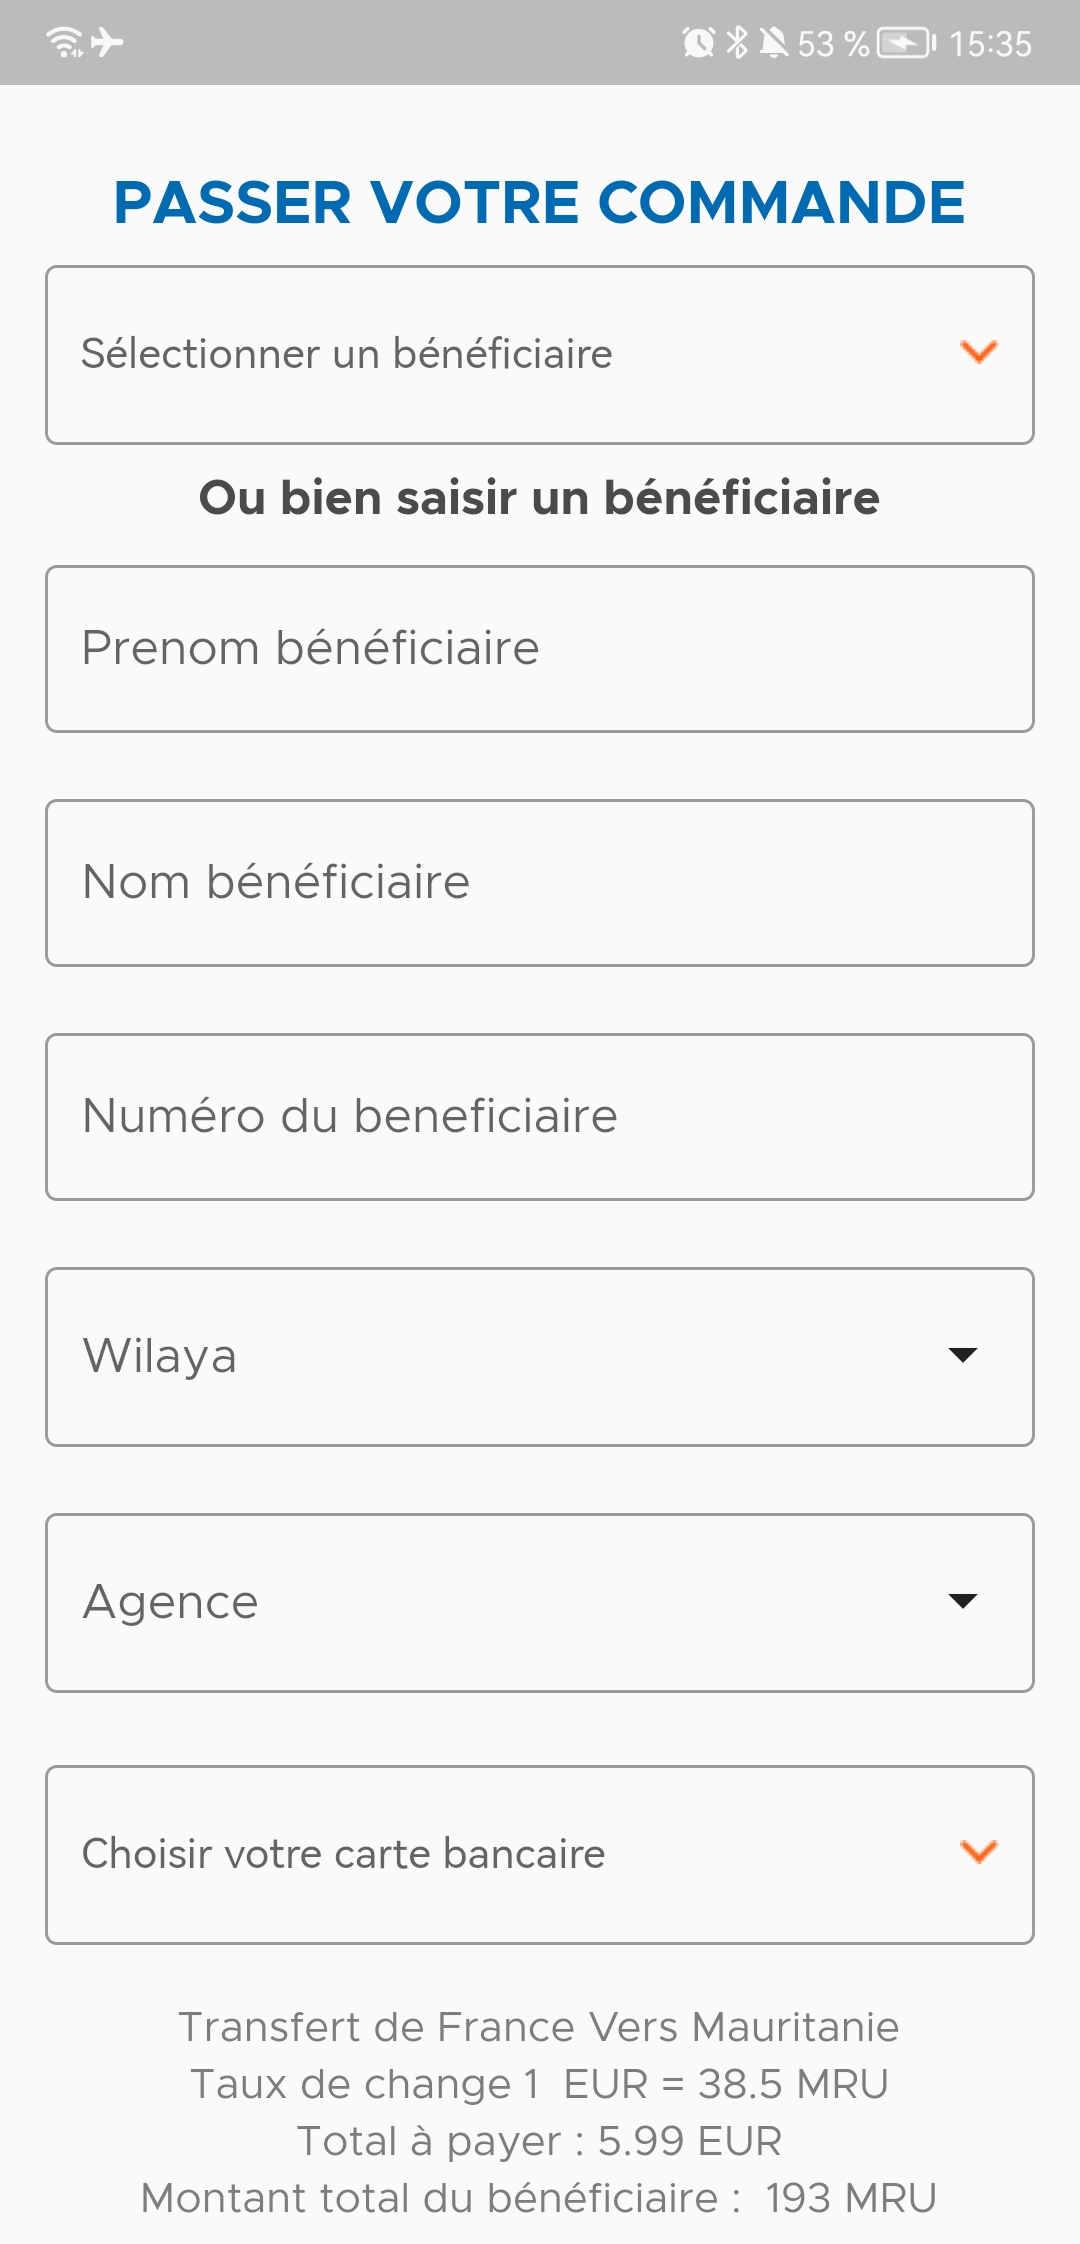
\includegraphics[width=\textwidth]{./Template LaTeX/Images/11.jpg}
		\caption{Interface de transfert}
		\label{fig:three sin x}
	\end{subfigure}
	\hfill
	\begin{subfigure}[b]{0.3\textwidth}
		\centering
		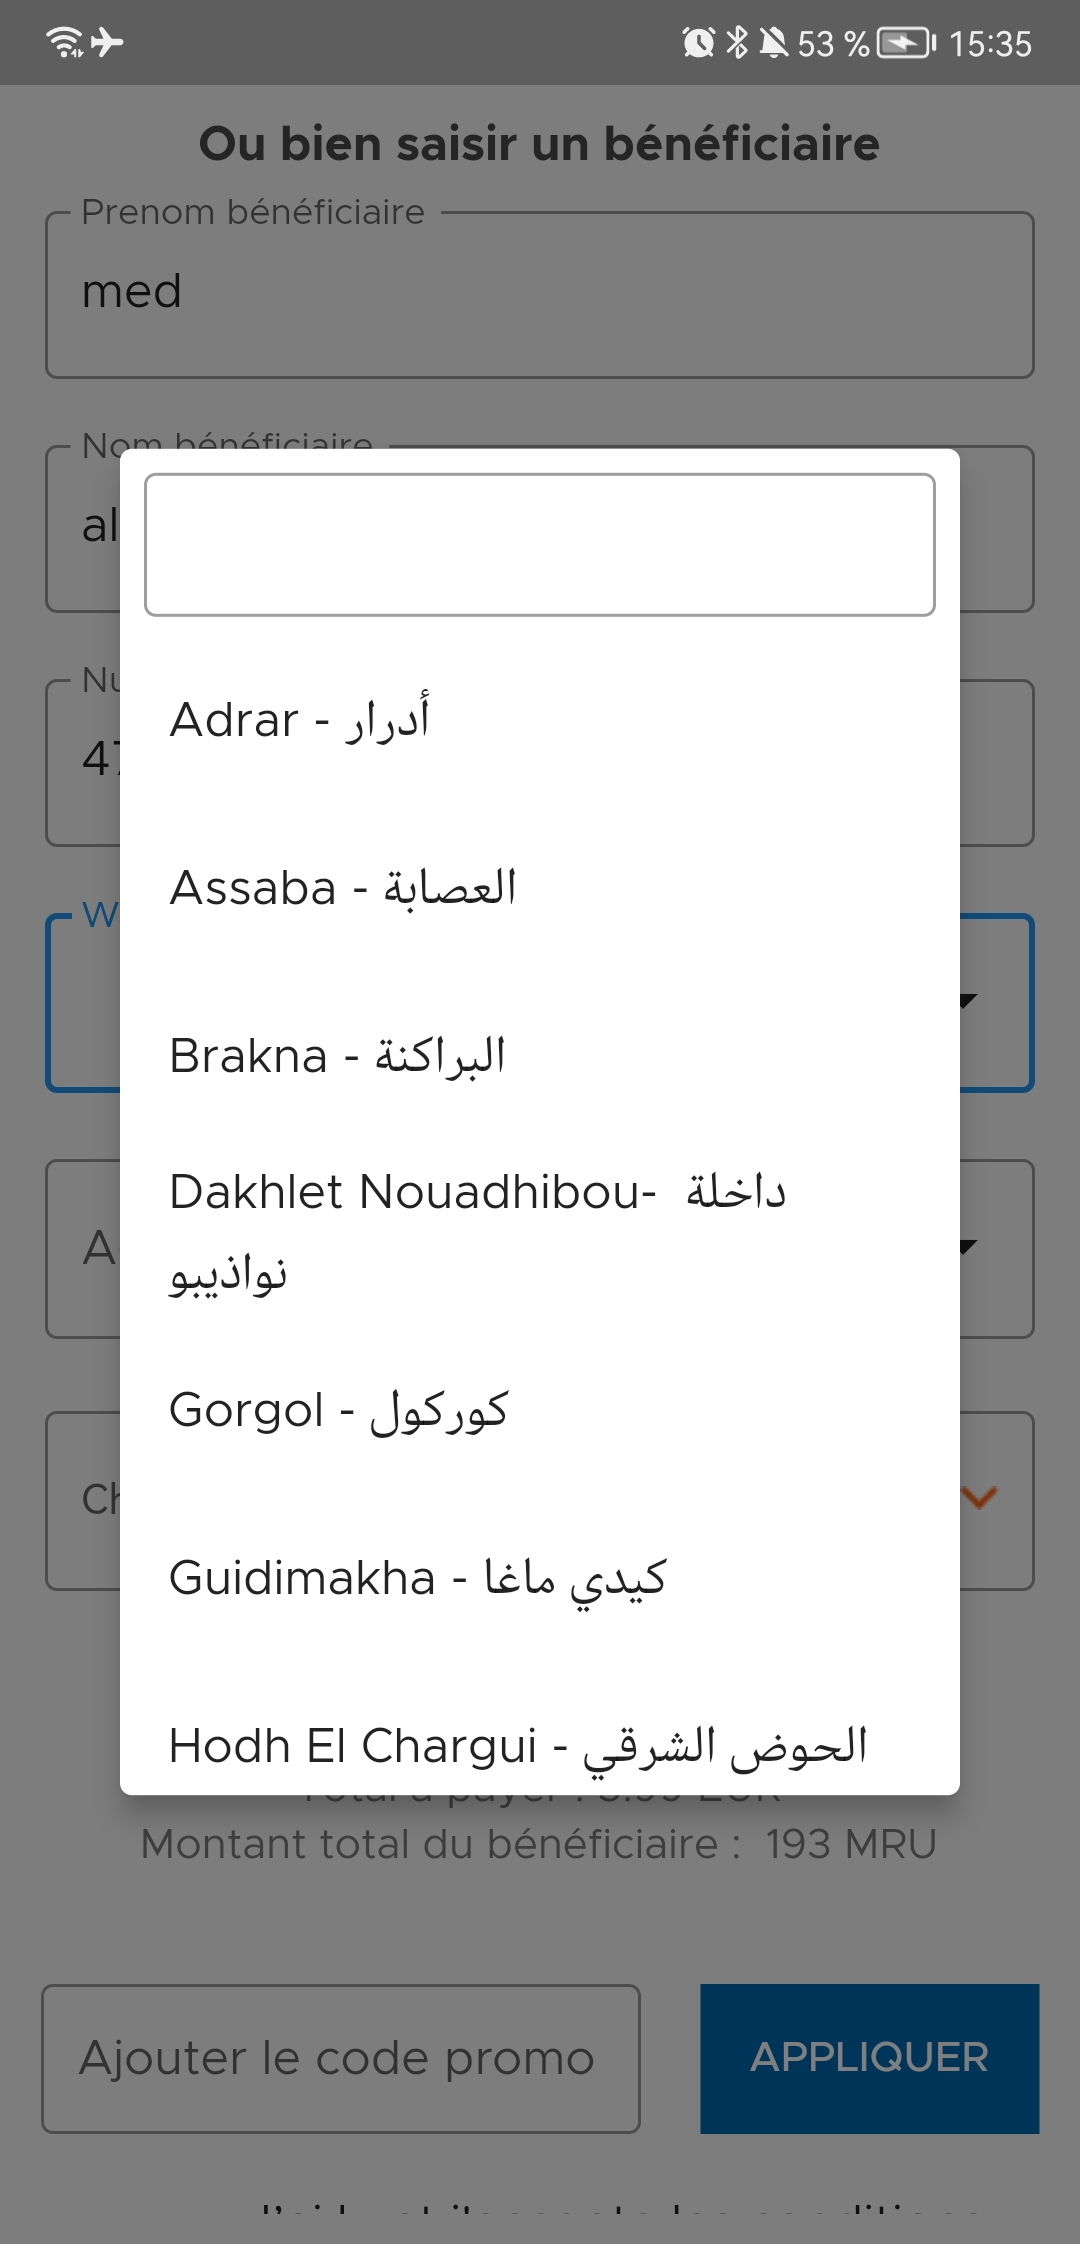
\includegraphics[width=\textwidth]{./Template LaTeX/Images/12.jpg}
		\caption{Choix de wilaya}
		\label{fig:five over x}
	\end{subfigure}
	\newline
		\centering
	\begin{subfigure}[b]{0.3\textwidth}
		\centering
		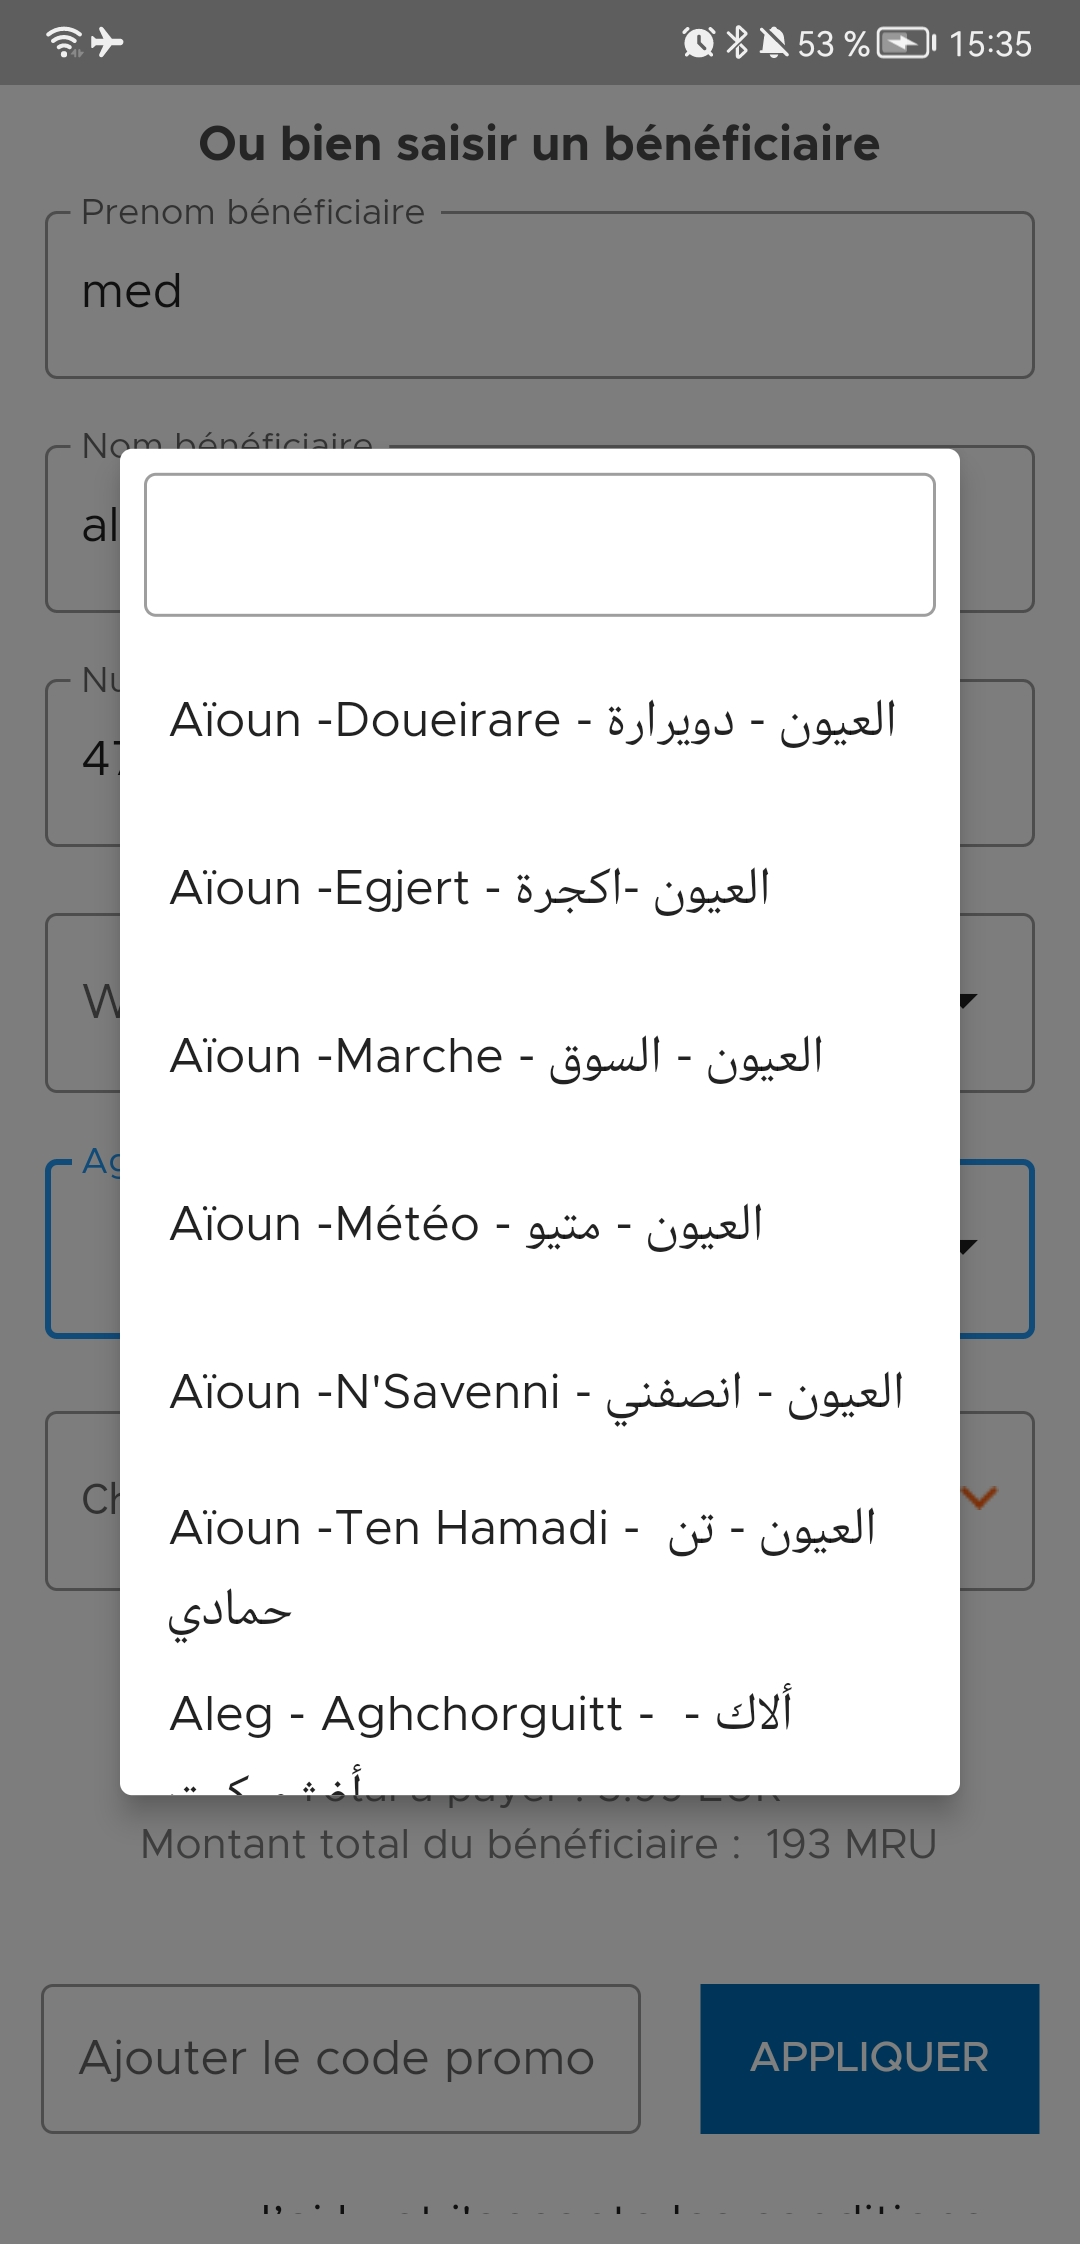
\includegraphics[width=\textwidth]{./Template LaTeX/Images/13.jpg}
		\caption{Choix d'agence}
		\label{fig:y equals x}
	\end{subfigure}
	\hfill
	\begin{subfigure}[b]{0.3\textwidth}
		\centering
		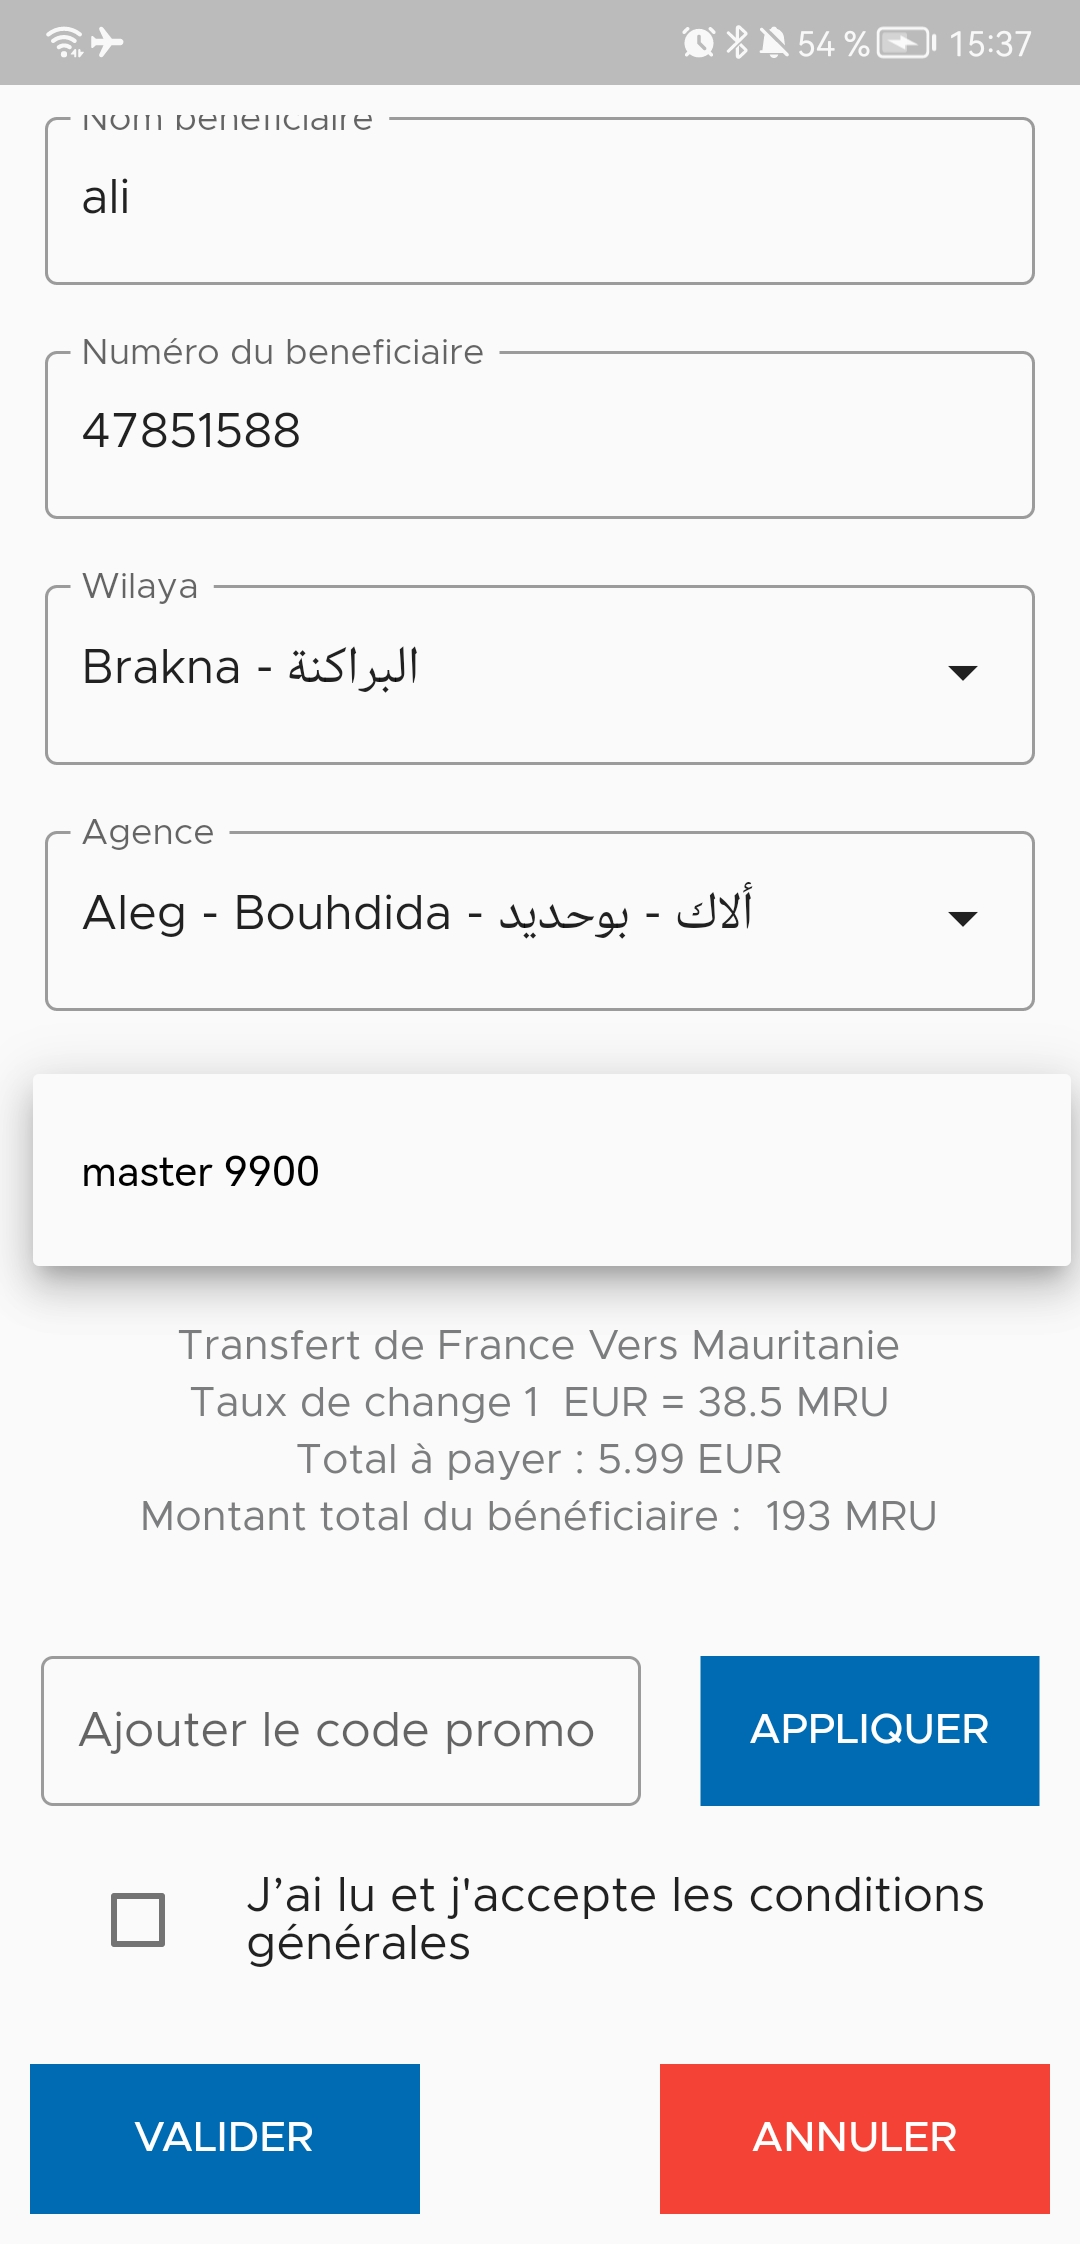
\includegraphics[width=\textwidth]{./Template LaTeX/Images/14.jpg}
		\caption{Choix de catre bancaire}
		\label{fig:three sin x}
	\end{subfigure}
	\hfill
	\begin{subfigure}[b]{0.3\textwidth}
		\centering
		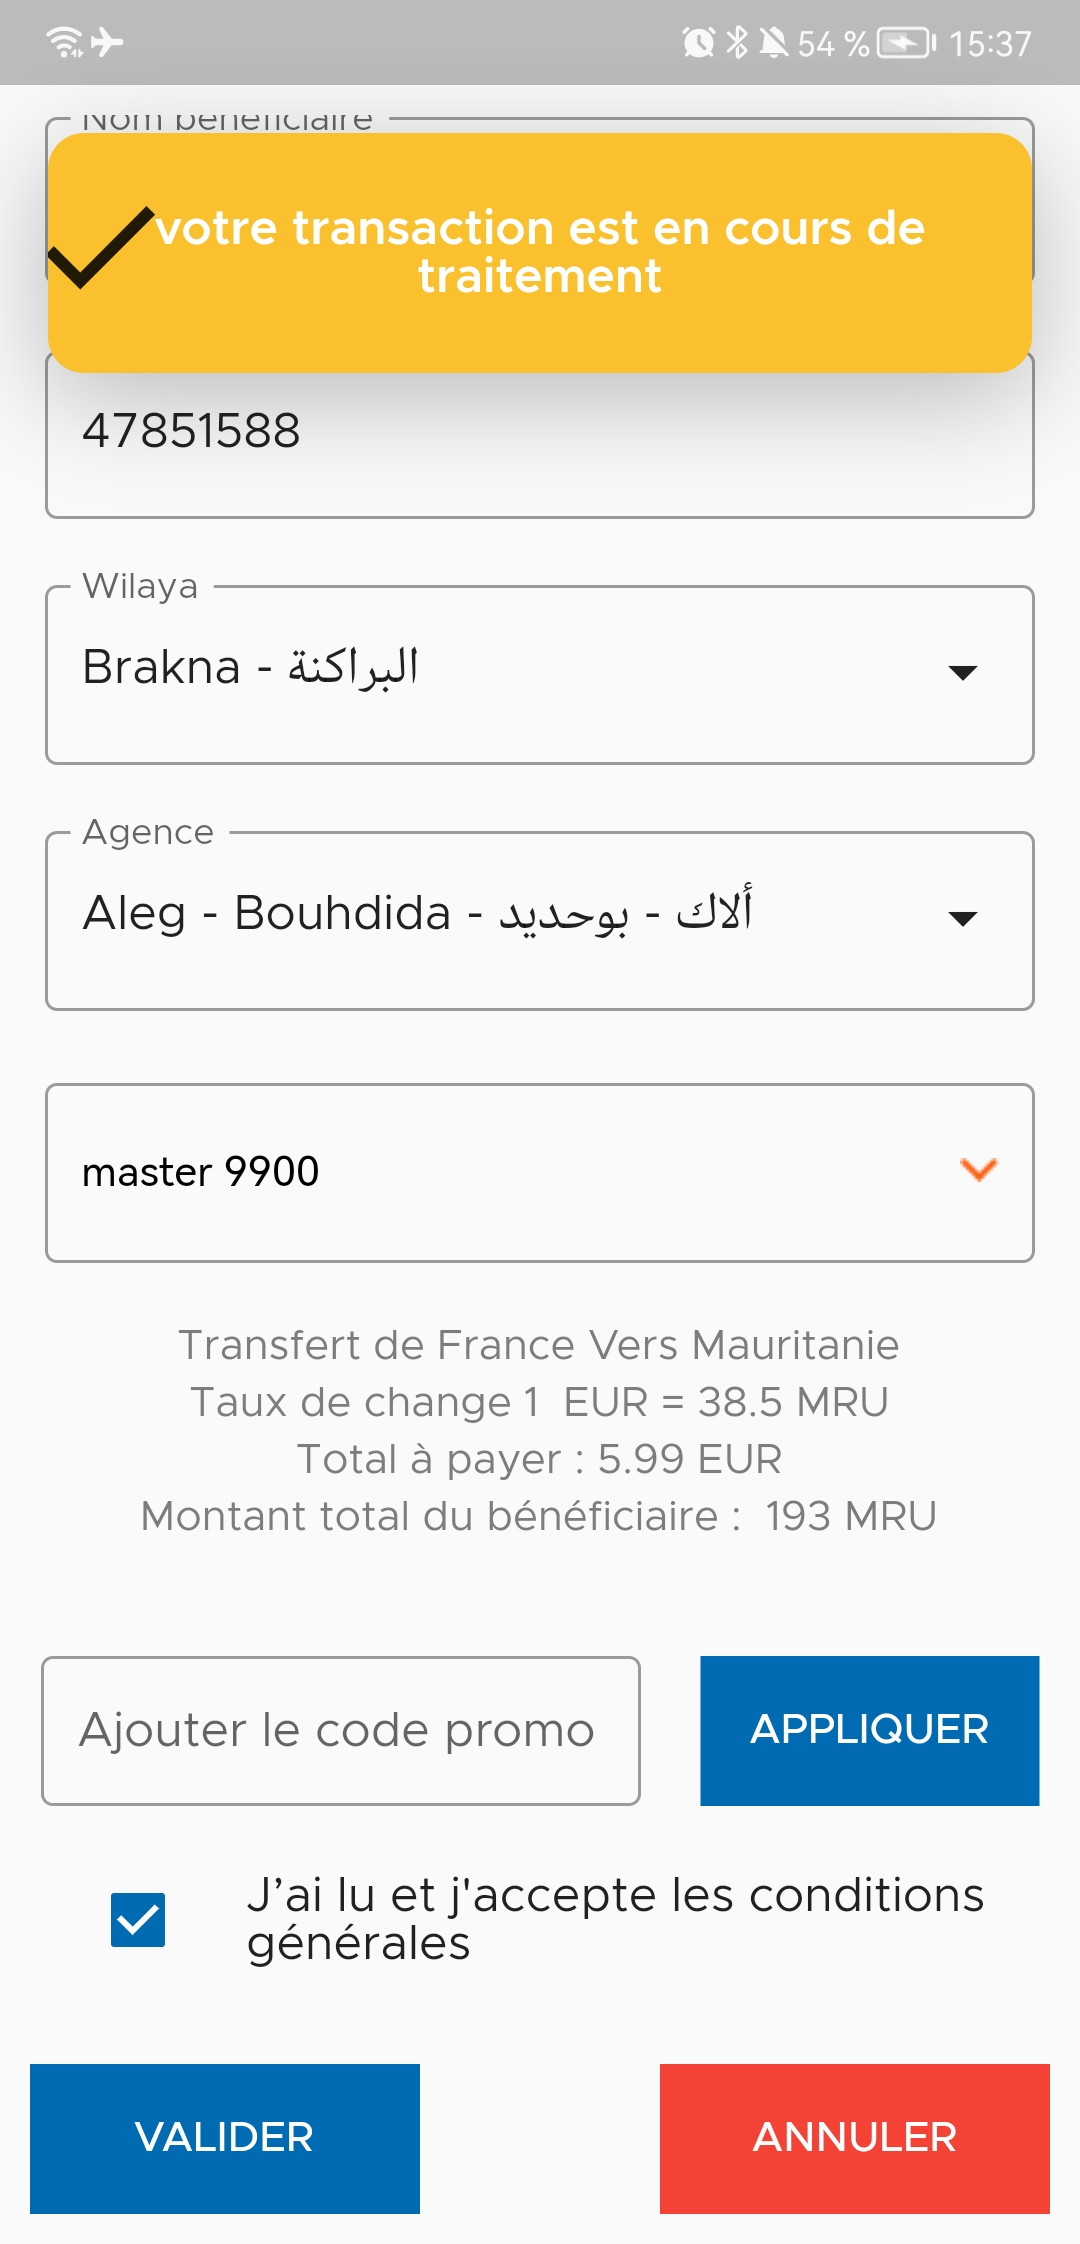
\includegraphics[width=\textwidth]{./Template LaTeX/Images/15.jpg}
		\caption{État de transfert}
		\label{fig:five over x}
	\end{subfigure}
	\caption{Processus de transactions}
	\label{fig:three graphs}
\end{figure}
\newpage
\item \textbf{L’interface de transfert
	:}La  \textbf{figure 4.7} montre l'historique des transactions de l'utilisateur  vers les bénéficiaires avec détails pour chaque transaction.

\begin{figure}
	\centering
	\begin{subfigure}[b]{0.3\textwidth}
		\centering
		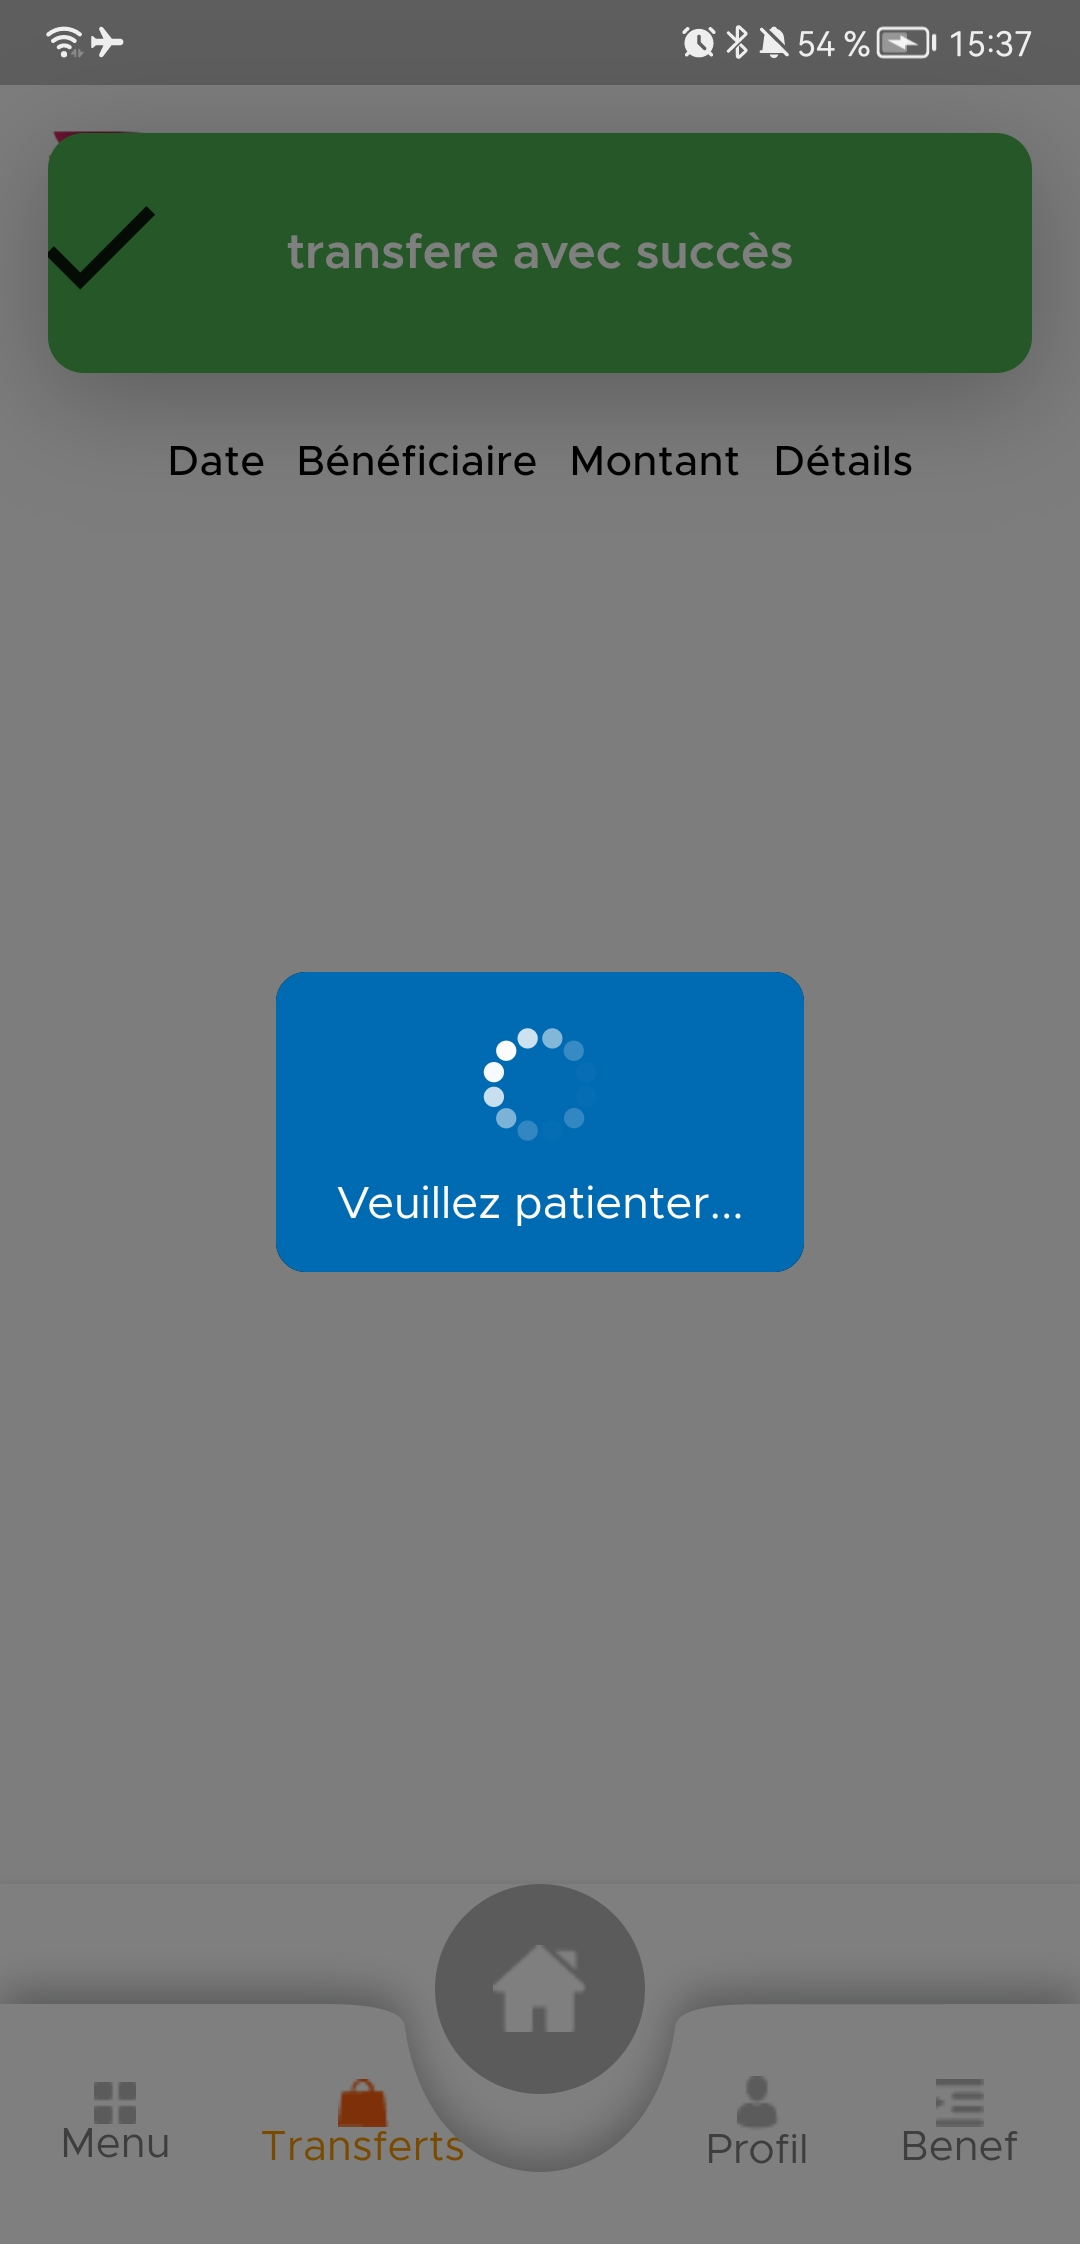
\includegraphics[width=\textwidth]{./Template LaTeX/Images/16.jpg}
		\caption{Transfere avec succés}
		\label{fig:y equals x}
	\end{subfigure}
	\hfill
	\begin{subfigure}[b]{0.3\textwidth}
		\centering
		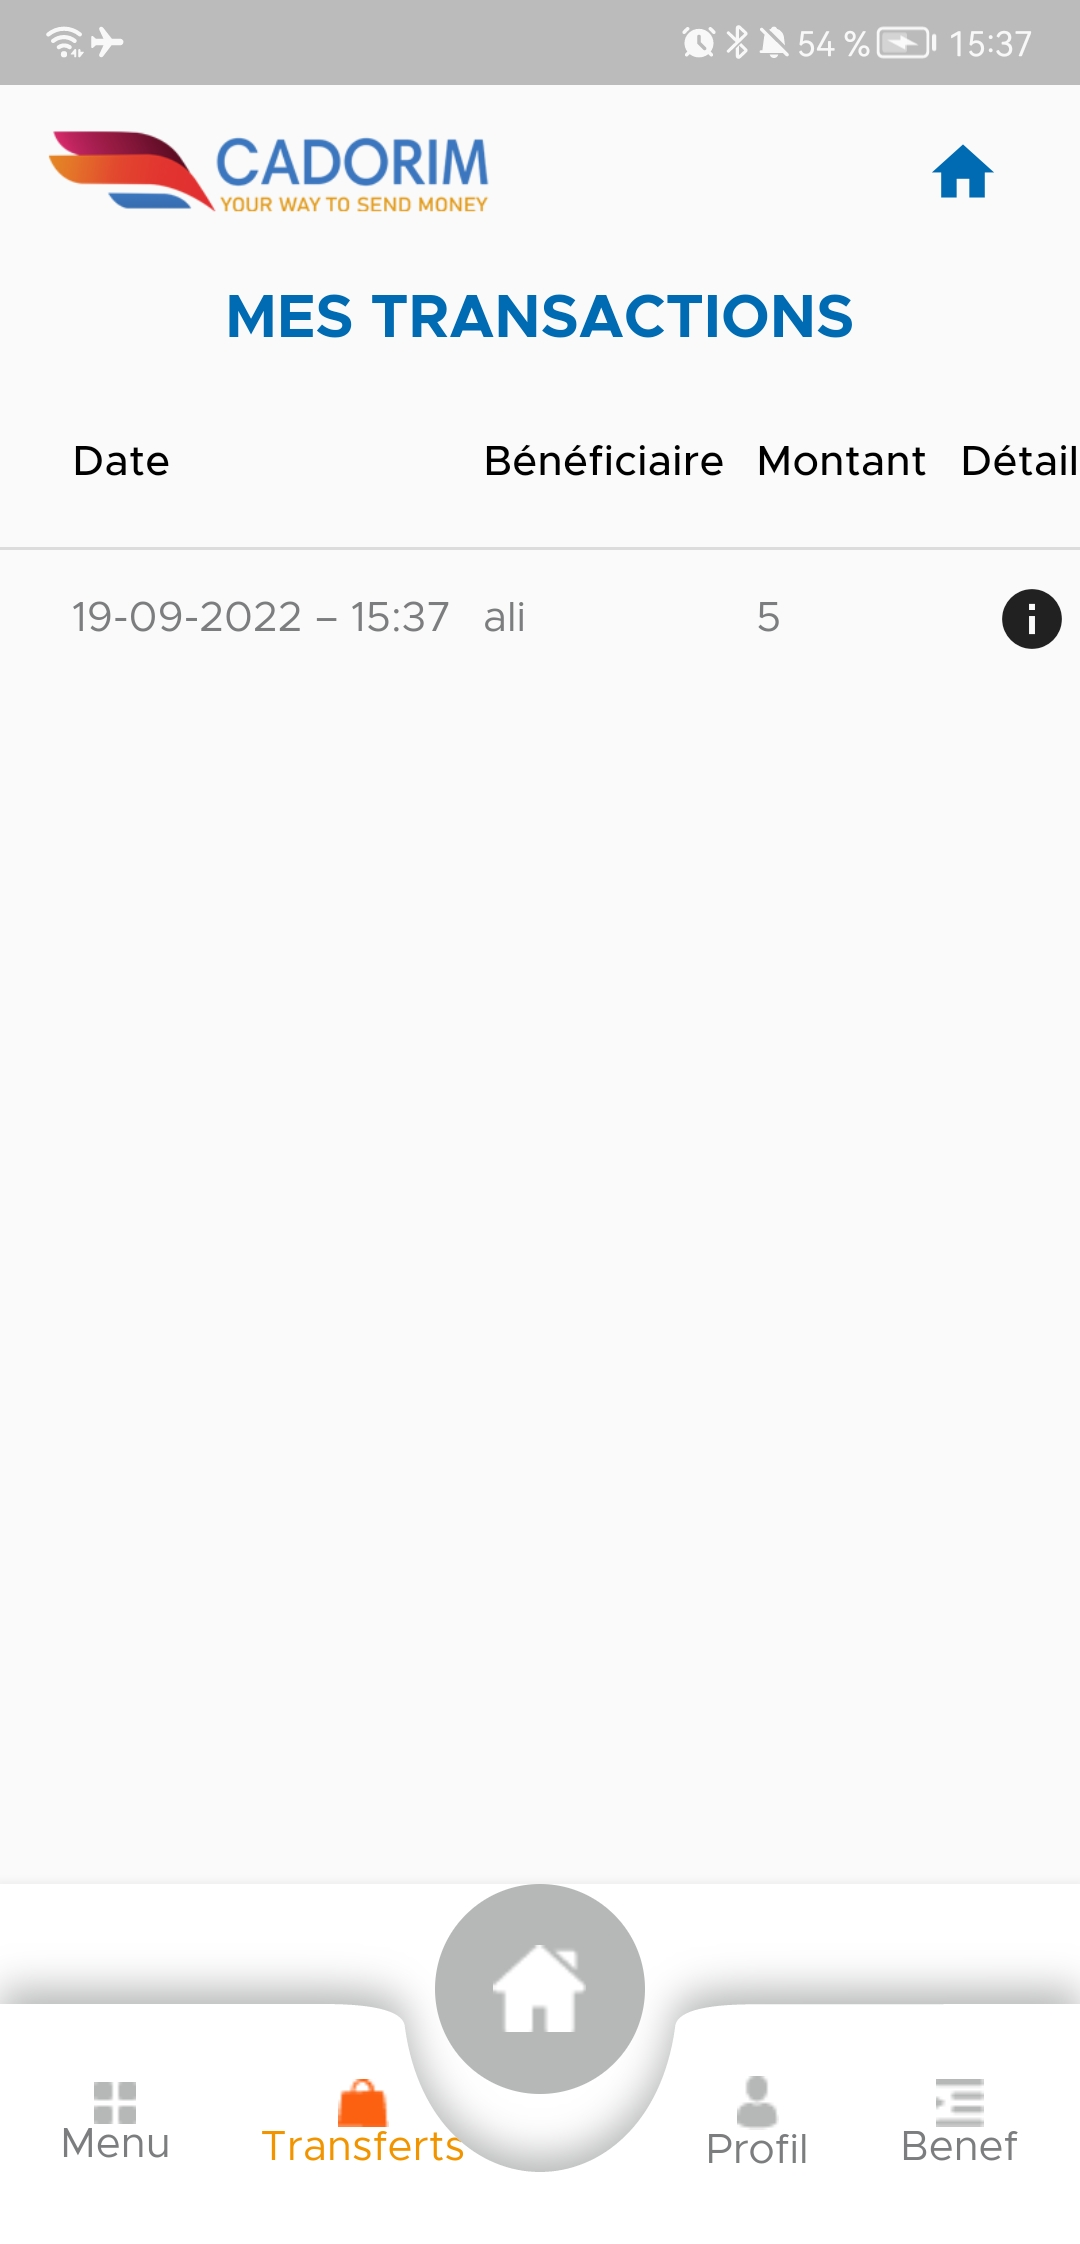
\includegraphics[width=\textwidth]{./Template LaTeX/Images/17.jpg}
		\caption{Historique transactions}
		\label{fig:three sin x}
	\end{subfigure}
	\hfill
	\begin{subfigure}[b]{0.3\textwidth}
		\centering
		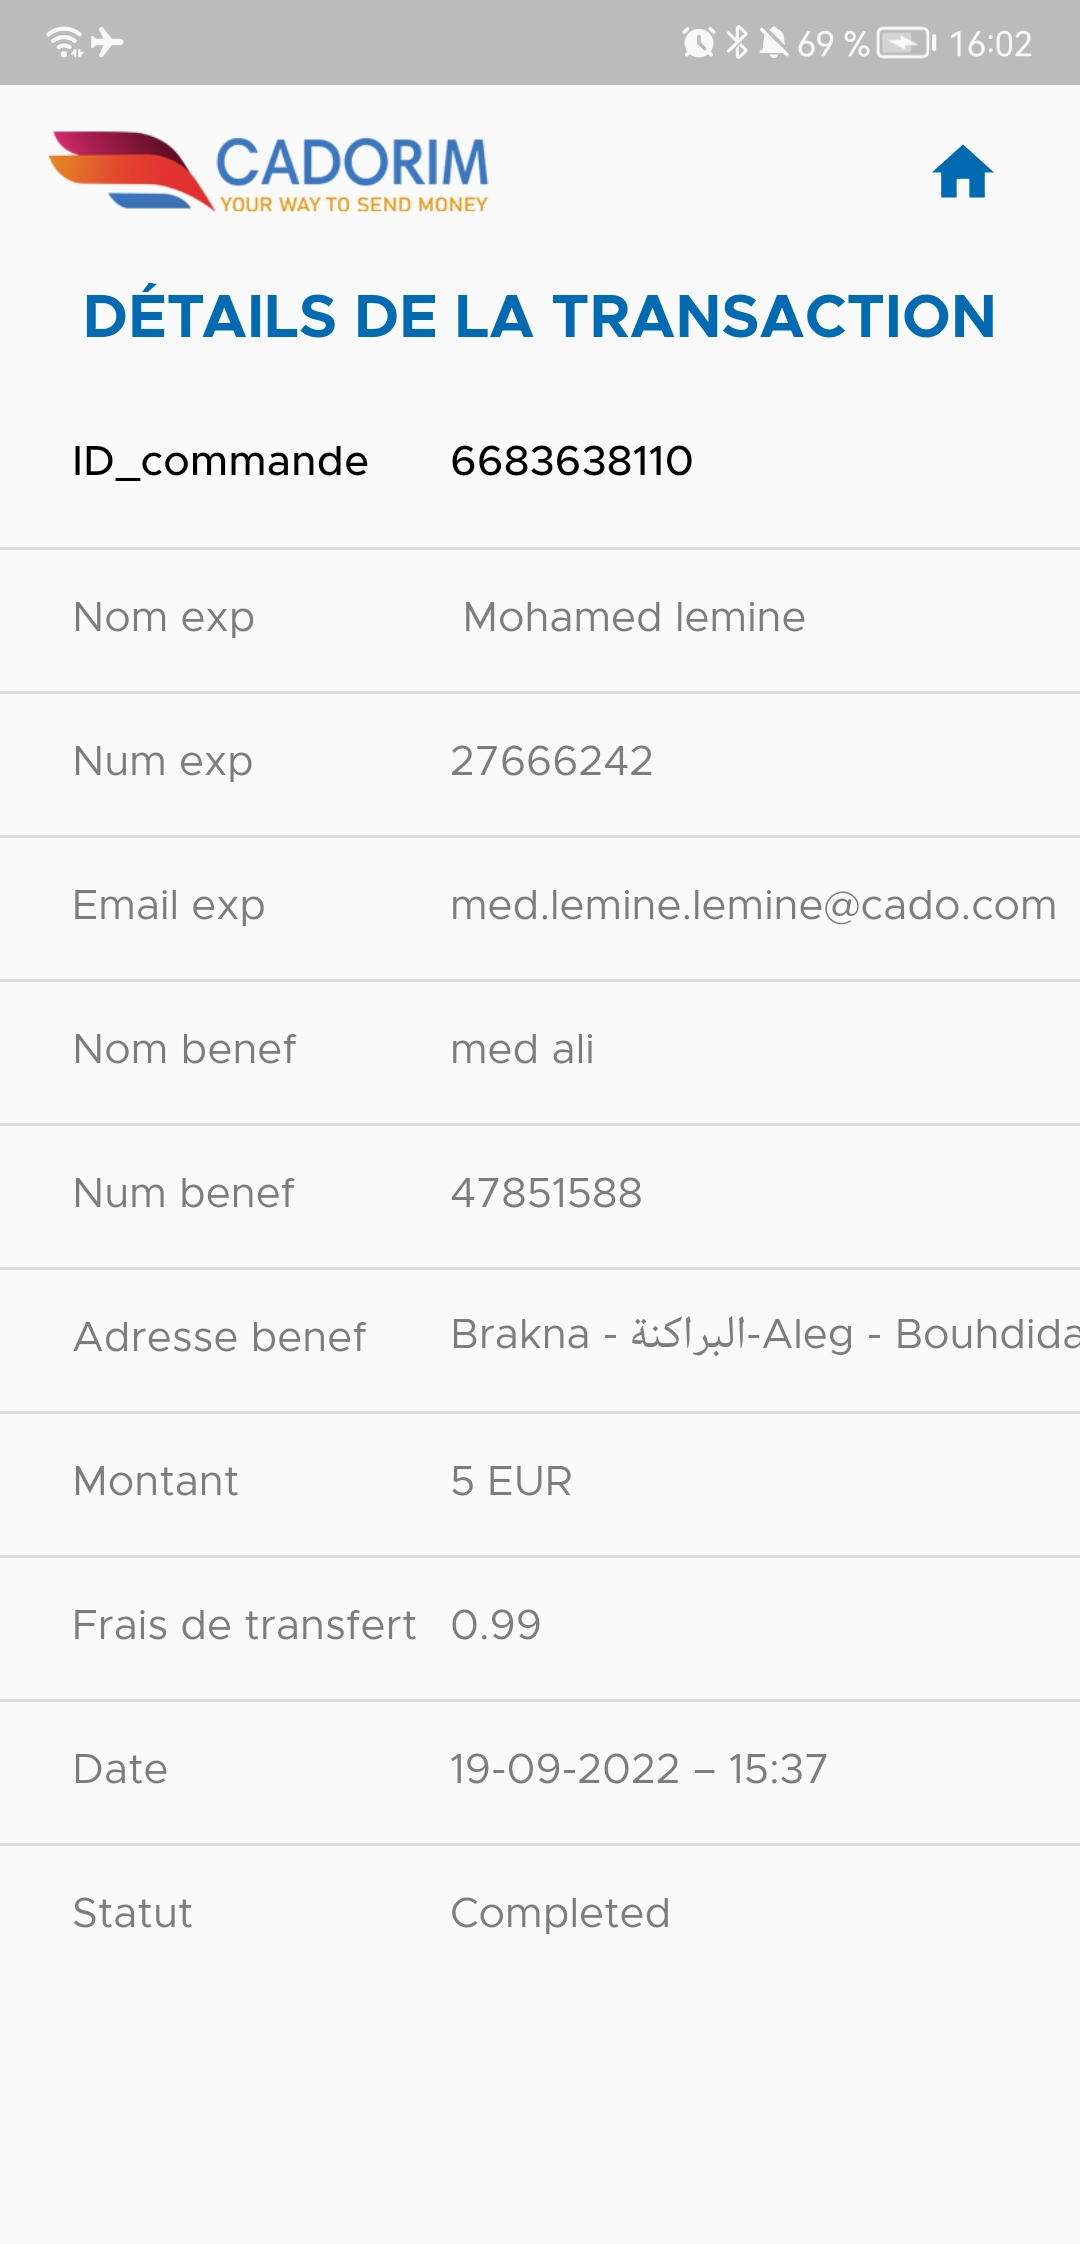
\includegraphics[width=\textwidth]{./Template LaTeX/Images/18.jpg}
		\caption{Détails de la transaction}
		\label{fig:five over x}
	\end{subfigure}
	\caption{Transferts}
	\label{fig:three graphs}
\end{figure}

\item \textbf{L’interface de discussion
	:} La figure suivante montre que le client peut envoyer un message (photo ou un texte) au service client et bien sur voir l'historique des messages.
	\begin{figure}%
	\centering
	{{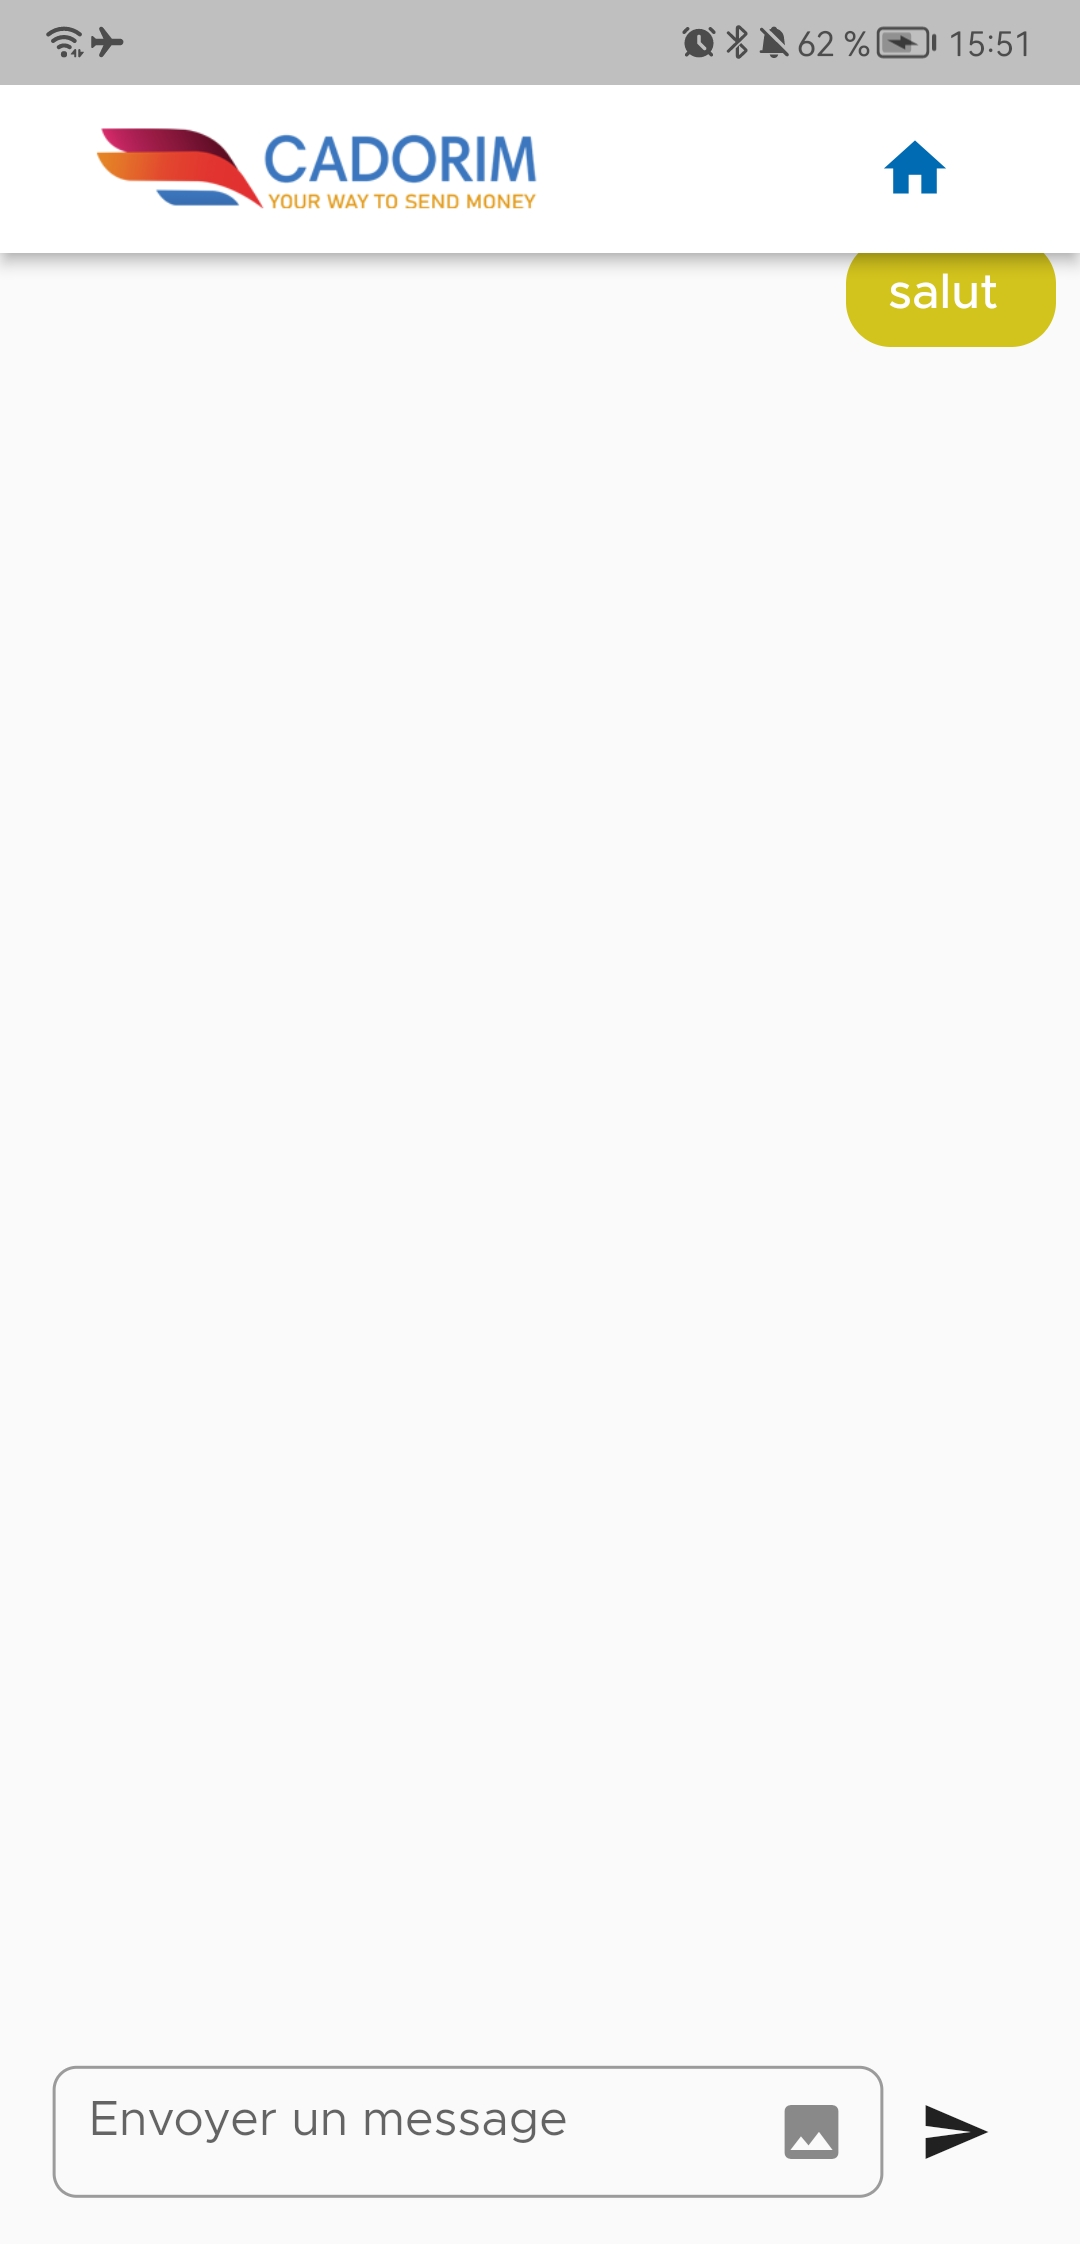
\includegraphics[width=5cm]{./Template LaTeX/Images/21.jpg} }}%
	\caption{Interface de discussion}%
	\label{fig:example}%
\end{figure}
\newpage
\item \textbf{Profil de l'utilisateur:} L'utilisateur peut mettre à jour leur profil ou ajouter un mode paiement comme il montre la figure suivante
\begin{figure}
	\centering
	\begin{subfigure}[b]{0.3\textwidth}
		\centering
		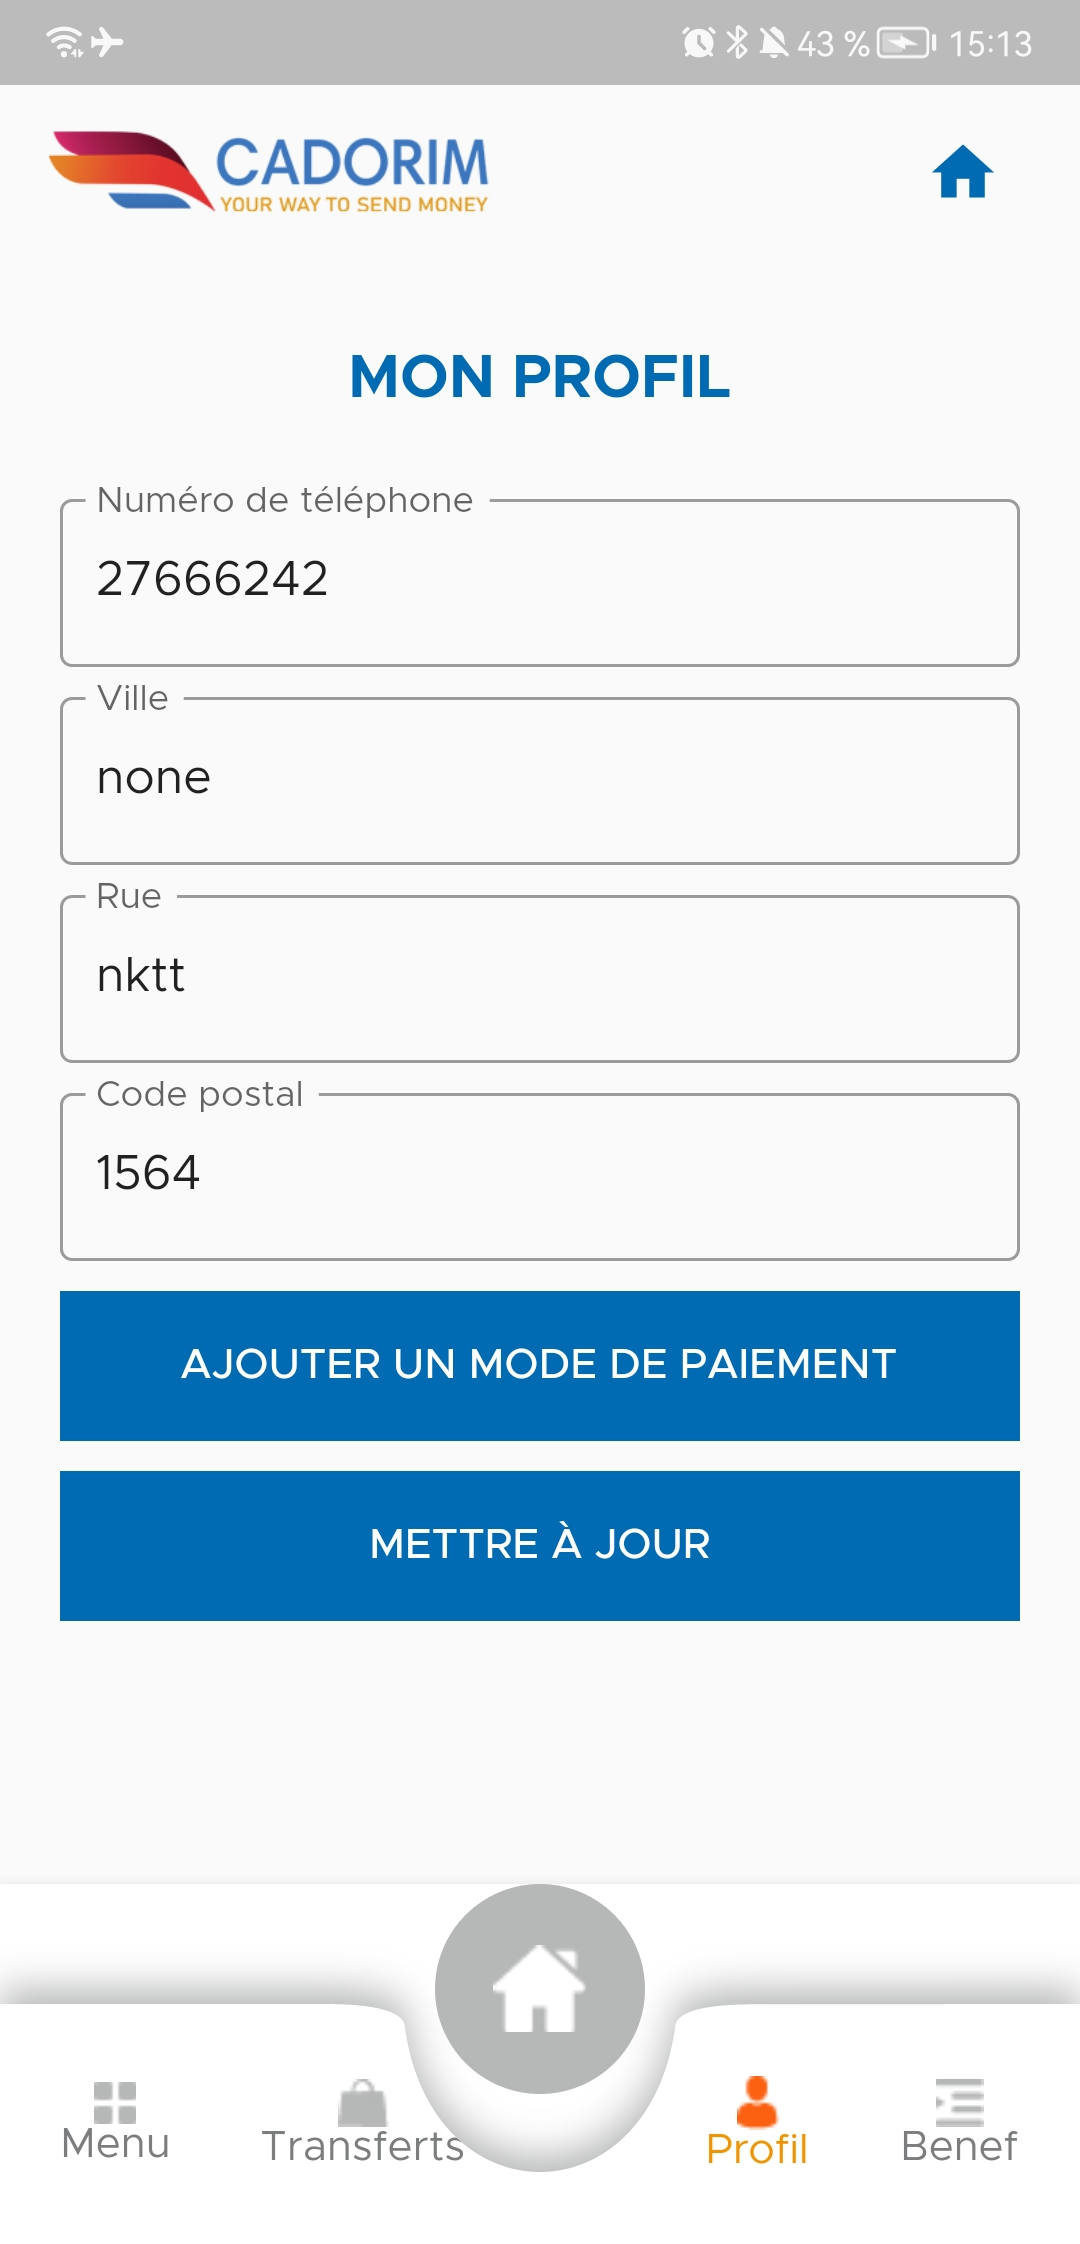
\includegraphics[width=\textwidth]{./Template LaTeX/Images/6.jpg}
		\caption{Mon profil}
		\label{fig:y equals x}
	\end{subfigure}
	\hfill
	\begin{subfigure}[b]{0.3\textwidth}
		\centering
		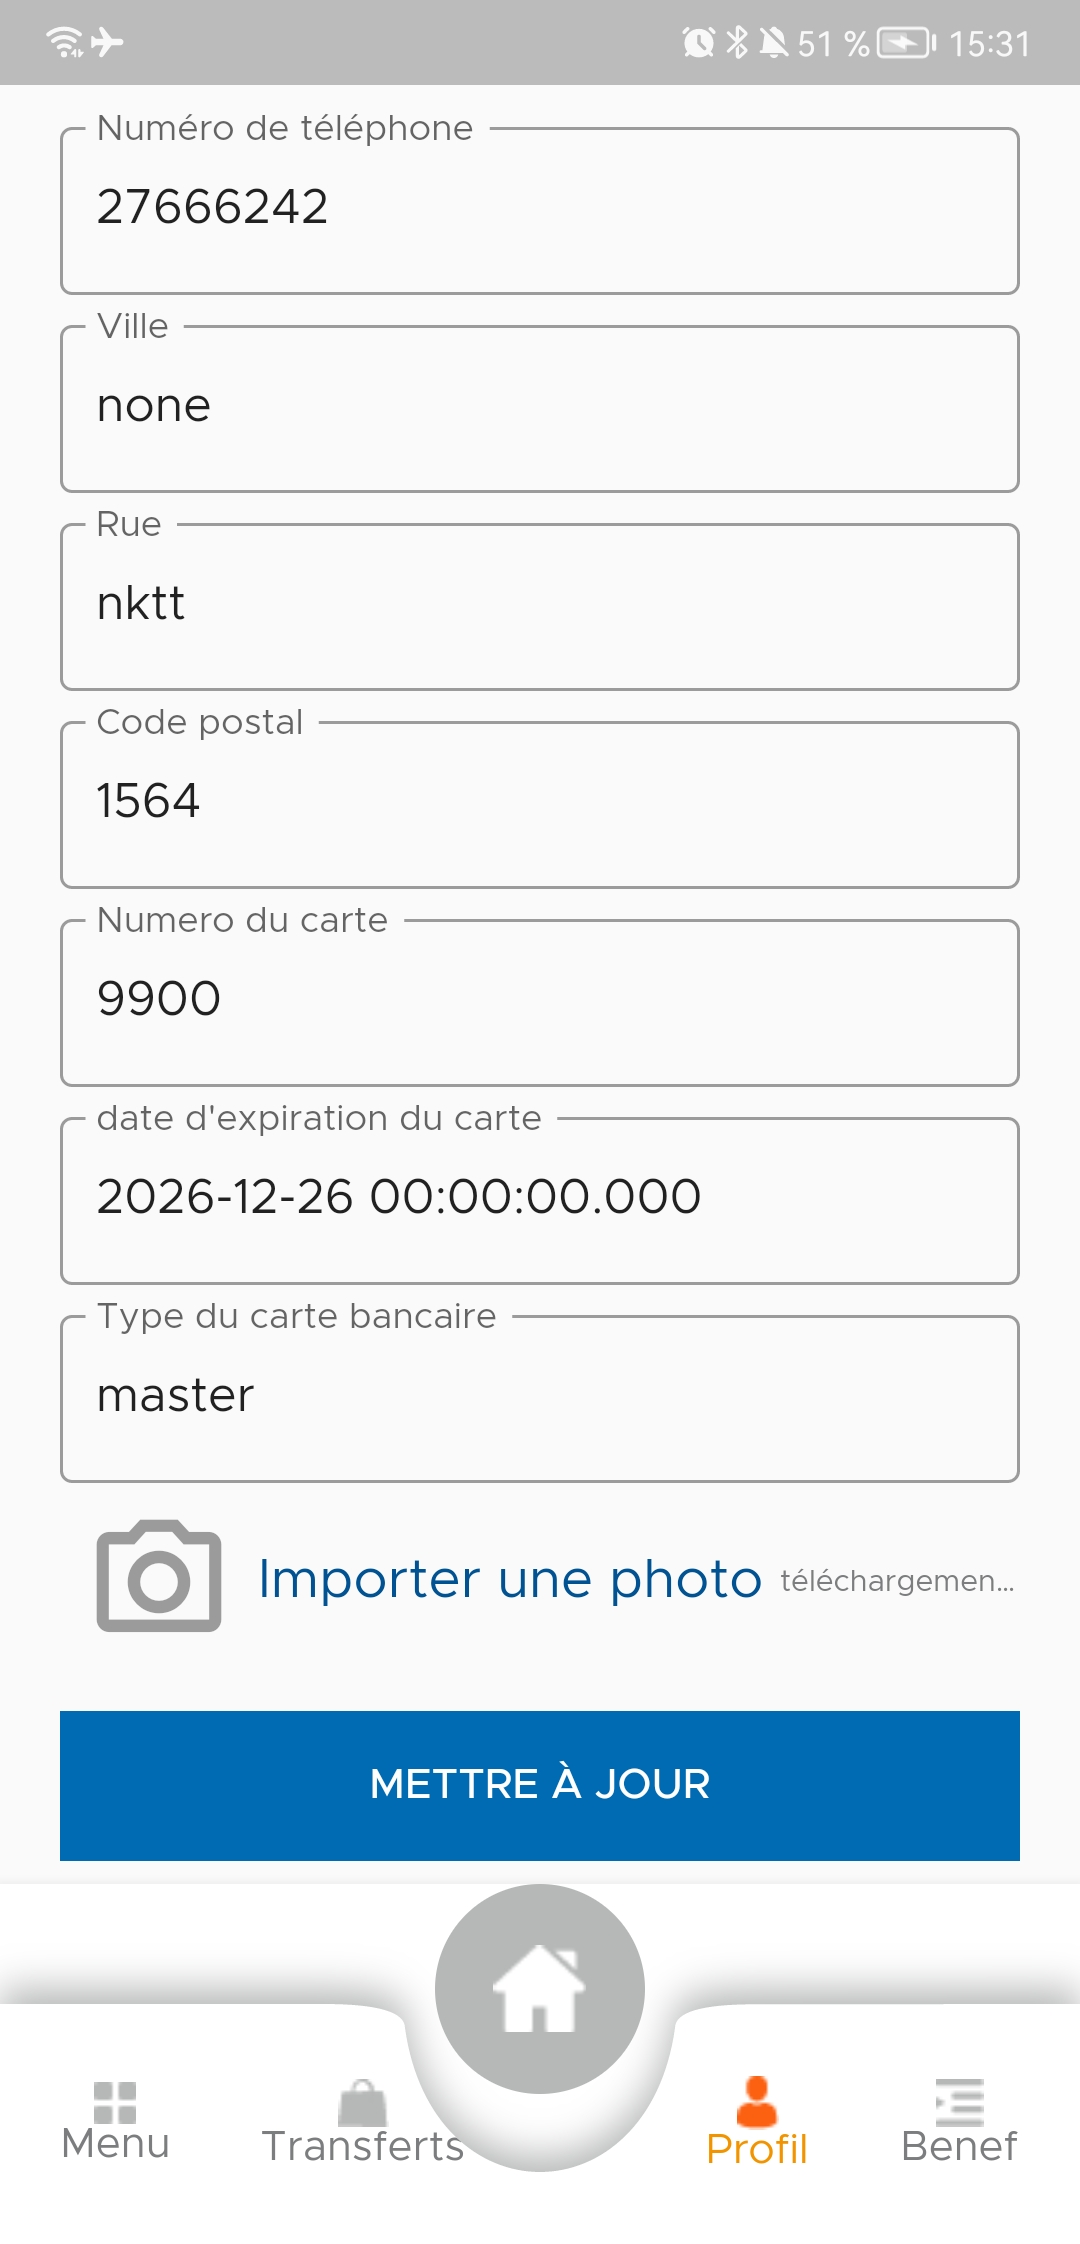
\includegraphics[width=\textwidth]{./Template LaTeX/Images/7.jpg}
		\caption{Ajouter une carte}
		\label{fig:three sin x}
	\end{subfigure}
	\hfill
	\begin{subfigure}[b]{0.3\textwidth}
		\centering
		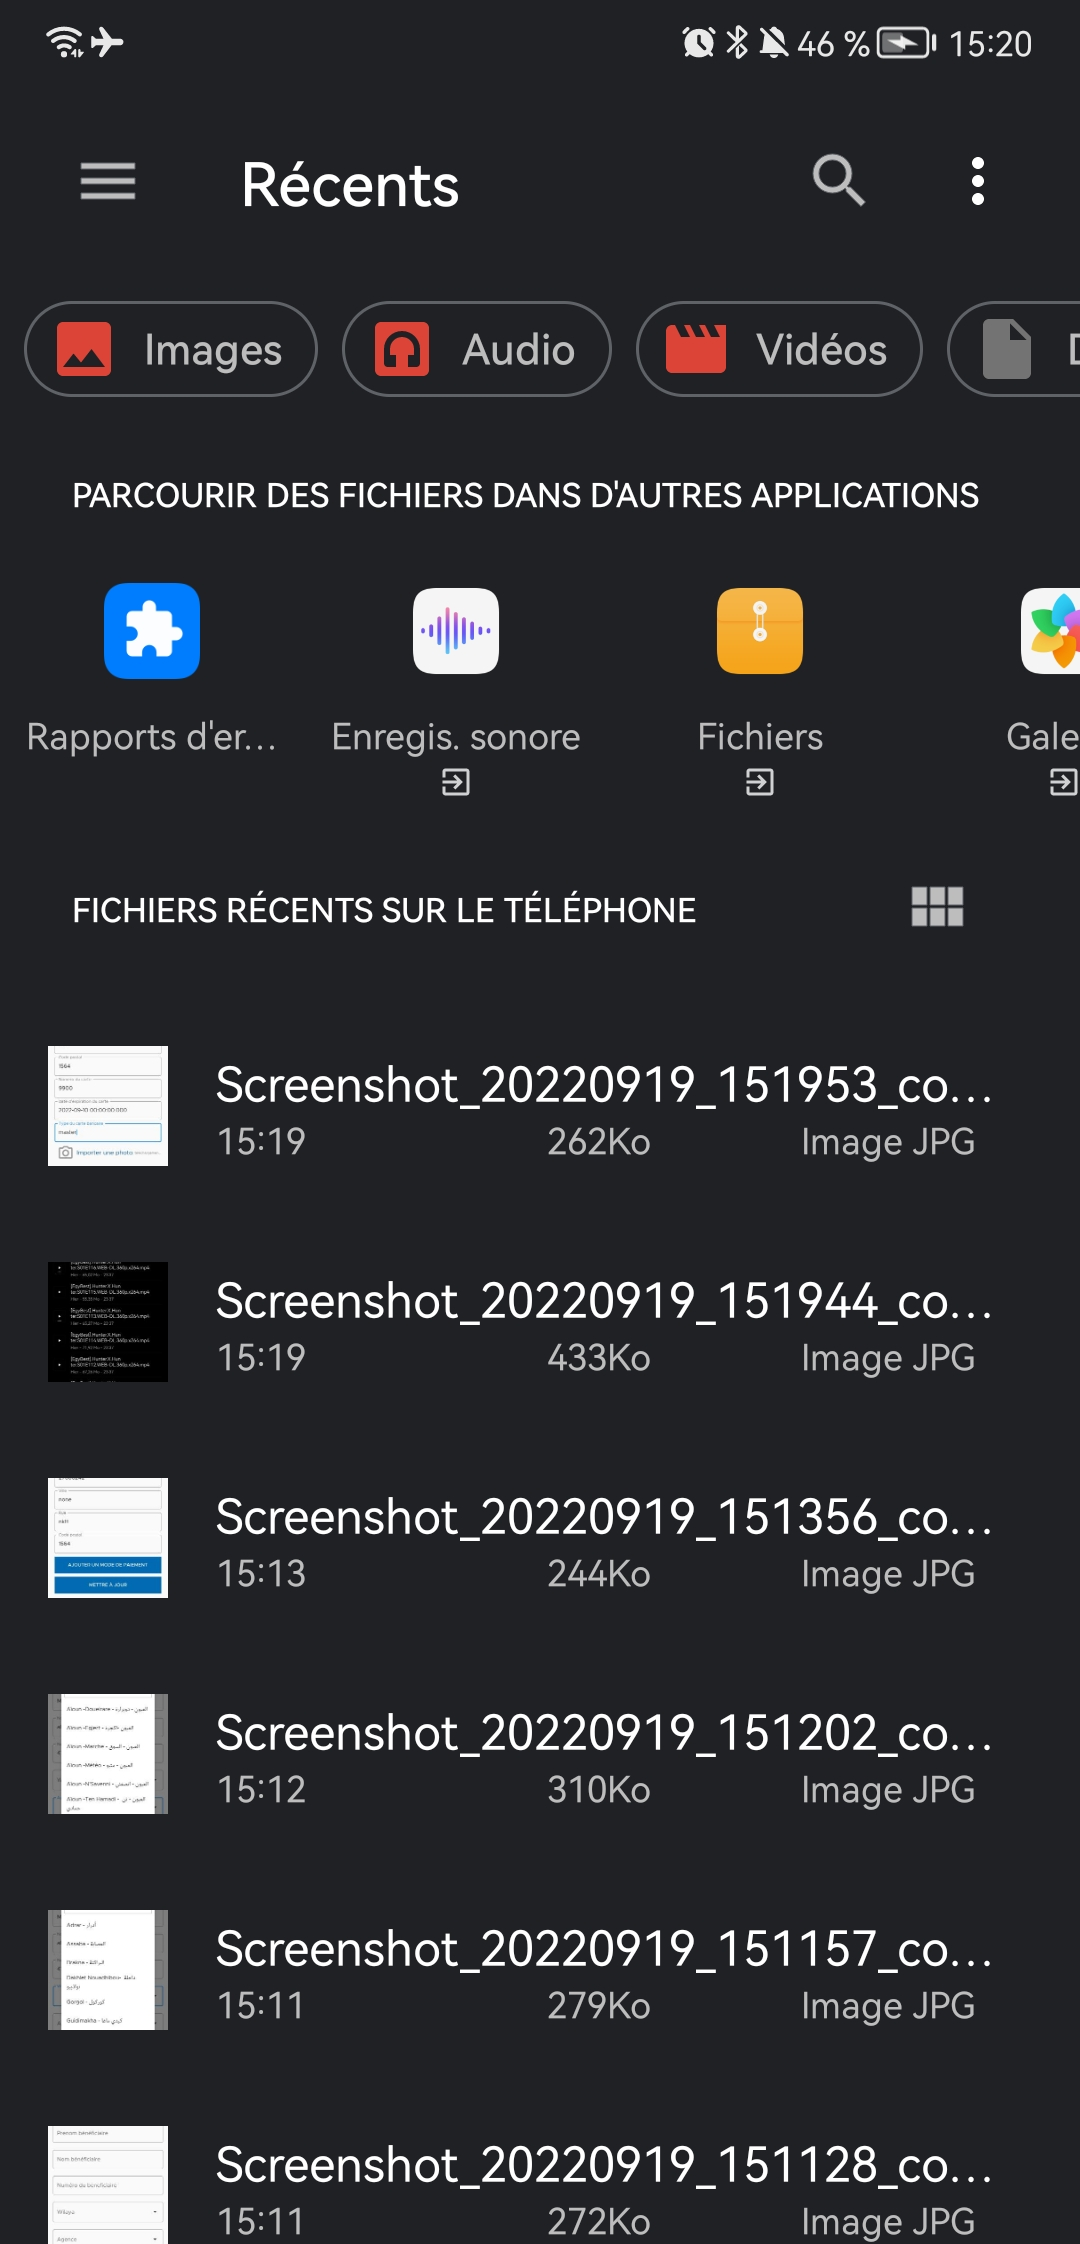
\includegraphics[width=\textwidth]{./Template LaTeX/Images/8.jpg}
		\caption{Importer une photo}
		\label{fig:five over x}
	\end{subfigure}
\newline
	\centering
\begin{subfigure}{0.3\textwidth}
	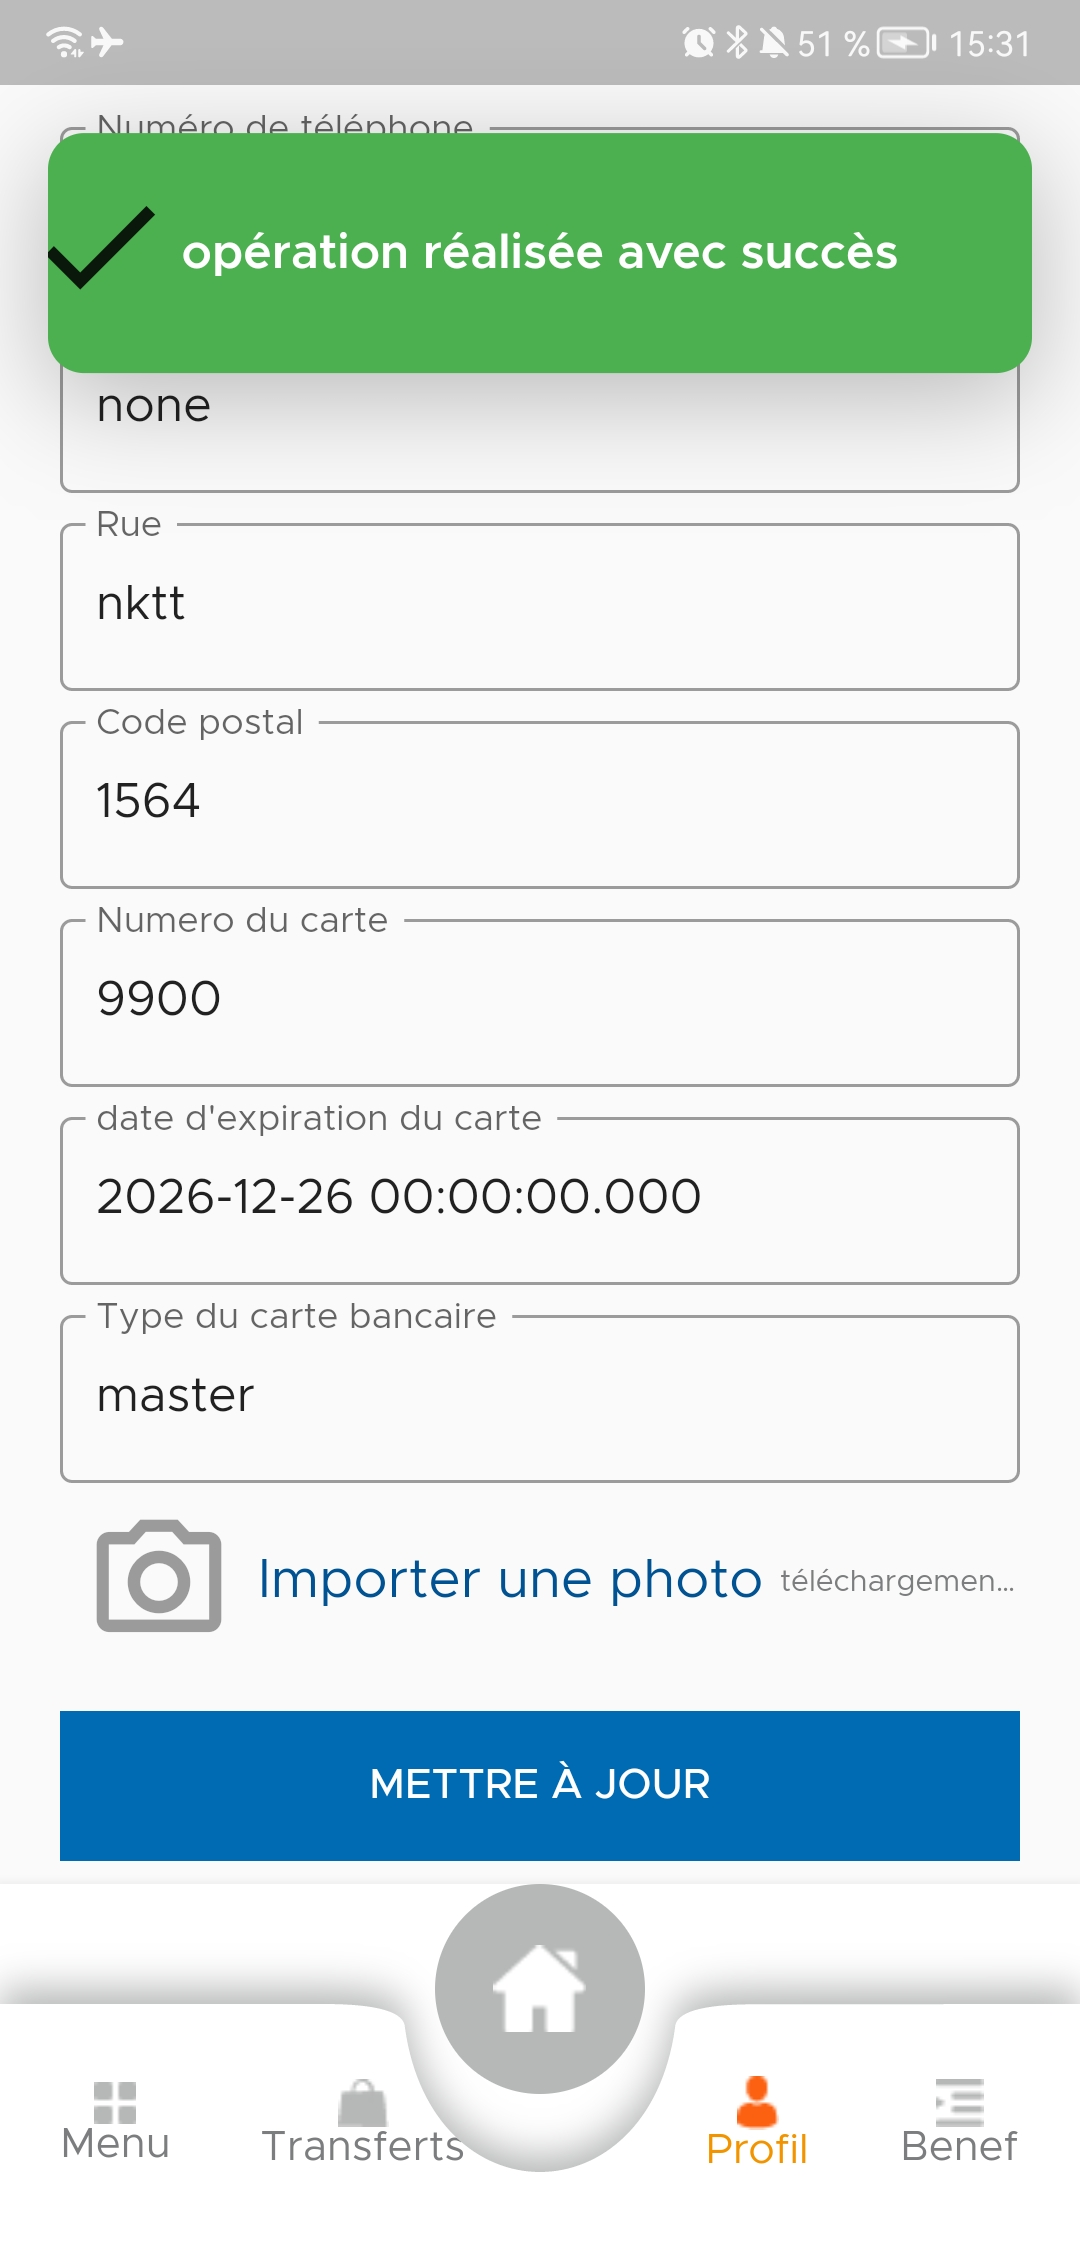
\includegraphics[width=\hsize, valign=m ]{./Template LaTeX/Images/9.jpg}
	\caption{État}
	\label{fig.SICAPI}
\end{subfigure}
%\qquad\tikz[baseline=-\baselineskip]\draw[ultra thick,->] (0,0) -- ++ (1,0);\qquad
\begin{subfigure}{0.3\textwidth}
	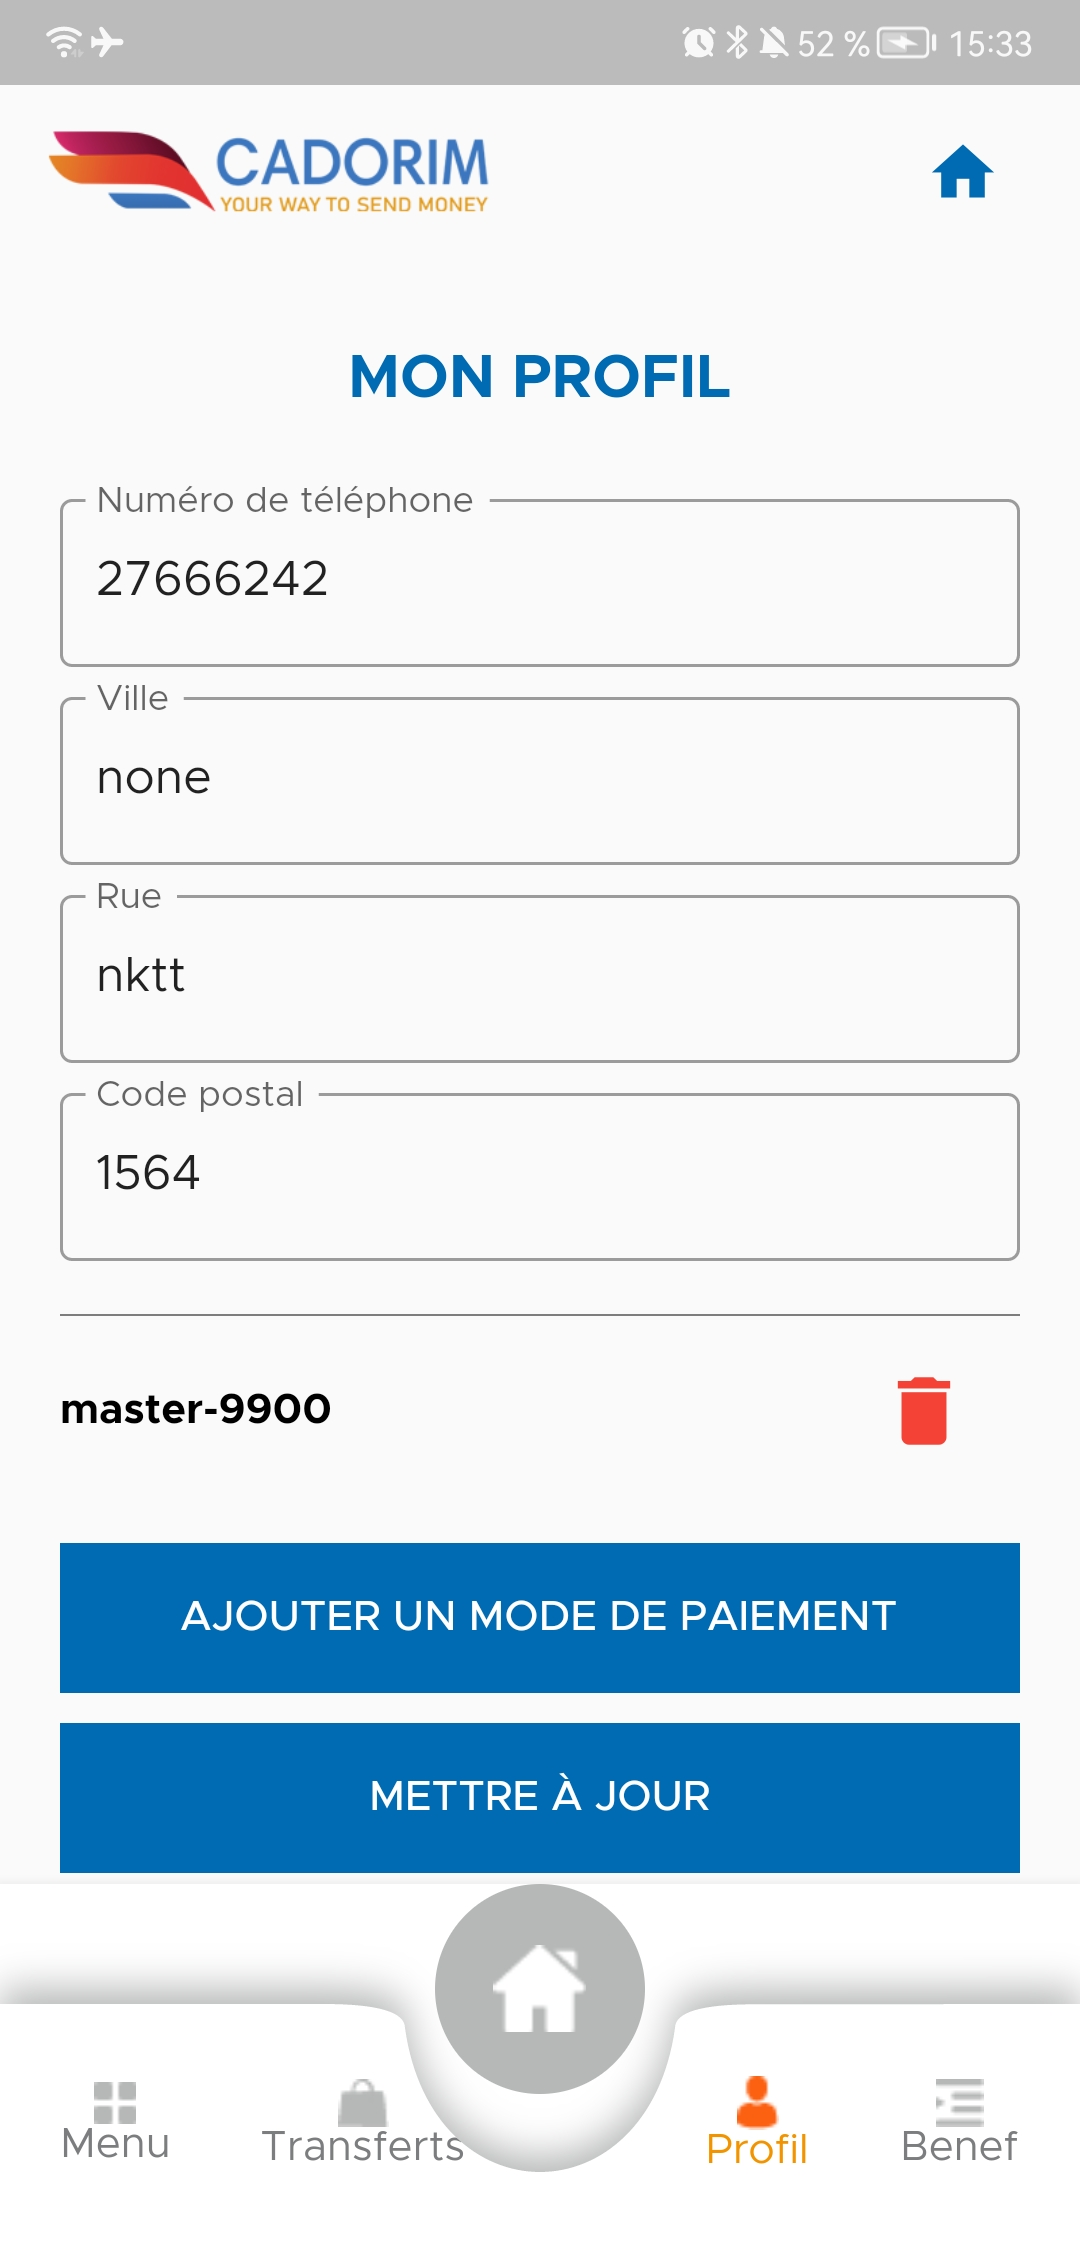
\includegraphics[width=\hsize, valign=m]{./Template LaTeX/Images/10.jpg}
	\caption{Interface suivante}
	\label{fig.painel_sicapi}
\end{subfigure}
	\caption{Profil de l'utilisateur
	}
	\label{fig:three graphs}
\end{figure}
\end{itemize}

\newpage
\subsubsection{Application ServiceClient}




	\chapter{Conclusion}
%	\chapter{Conclusion générale et perspectives}
	\chapter{Bibliographie}
	%\chapter{Implémentation}
Durant la réalisation de ce projet, nous avons essayé d’utiliser différents
outils de développement, d’une part afin de rendre la tâche de la
réalisation plus facile, d’autre part pour que notre système soit robuste et
répond parfaitement a nos besoins , et que nos interfaces soient claires et
faciles à utiliser.
\section{Architecture de l'application}
Cadorim est une application embarquée qui se connect à un serveur de base de données distant, via Internet, afin de récupérer les données, Ce qui necessite aussi l'intégration d'un serveur web entre l'application client et le serveur de bases de données.
D'où larchitecture de notre application est à 3 niveaux, elle est partagée entre;
\begin{enumerate}
	\item \textbf {L'application mobile (IOS ou Android) : }  Ce le client qui demande les ressources.
	\item \textbf{Le Serveur Web :} Vue que les données serons communiquées entre deux environnements hétérogènes, le rôle principale du serveur web est de gérer la communication entre le client (Android ou IOS) et le serveur de données.
	\item \textbf{Le serveur de base de données:} fournis les données au serveur web.
\end{enumerate}

\begin{figure}[h!]
	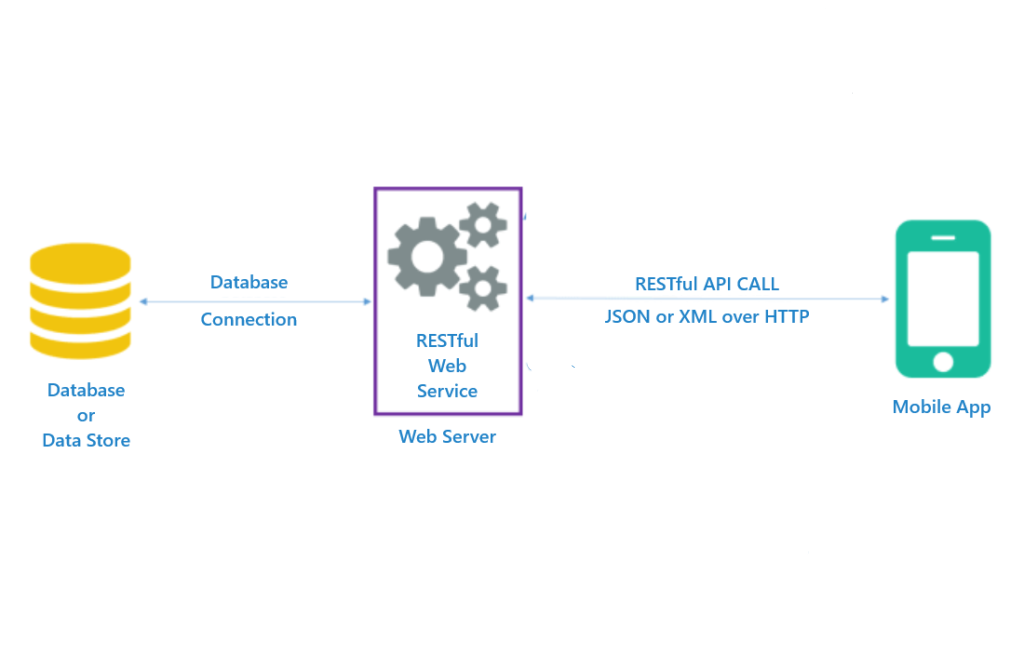
\includegraphics[width=17cm, height=10cm]{./Template LaTeX/Images/architect_after_edit.png}
	\caption{Architecture logicielle de l’application.}
	\label{fig:birds}
	
	
\end{figure}
\newpage
\section{Interfaces graphiques}
Les interfaces utilisateur doivent respecter les heuristiques d'utilité pour permettre à l'utilisateur un accès facile à ces interfaces afin de garantir une bonne compréhension des fonctionnalités de l'application. Nous présentons ici les interfaces les plus significatives de l'application.
\subsection{Interfaces d'acceil}

L'utilisateur du Cadorim avant d'être invite à consulter les services de l'application, doit 
choisies leur lange avant qu'il pass a l'interface suivante.

\begin{figure}[!ht]
	\centering
	\begin{subfigure}{0.3\textwidth}
		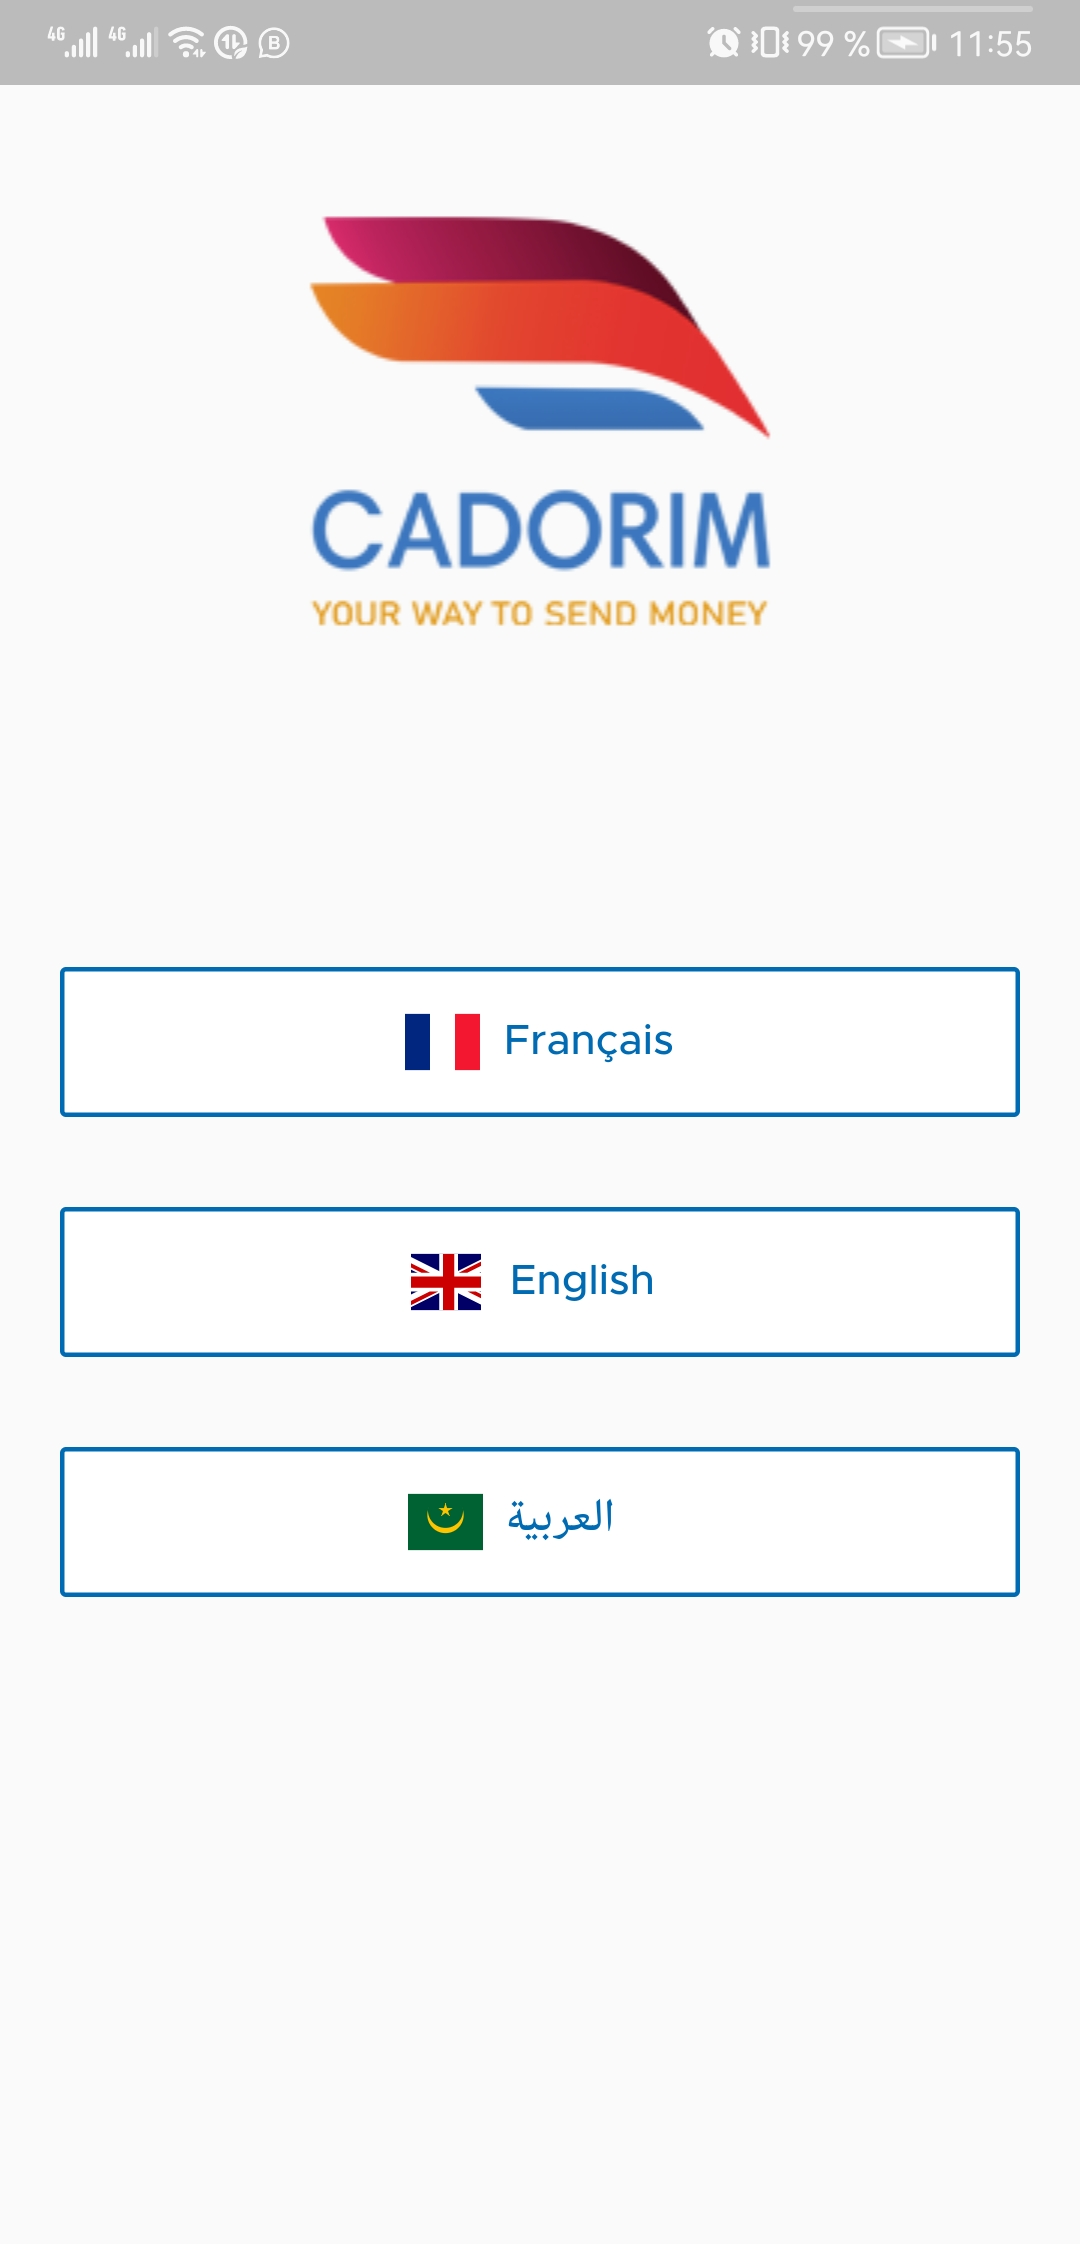
\includegraphics[width=\hsize, valign=m]{./Template LaTeX/Images/1.jpg}
		\caption{Choix de lange}
		\label{fig.SICAPI}
	\end{subfigure}
	\qquad\tikz[baseline=-\baselineskip]\draw[ultra thick,->] (0,0) -- ++ (1,0);\qquad
	\begin{subfigure}{0.3\textwidth}
		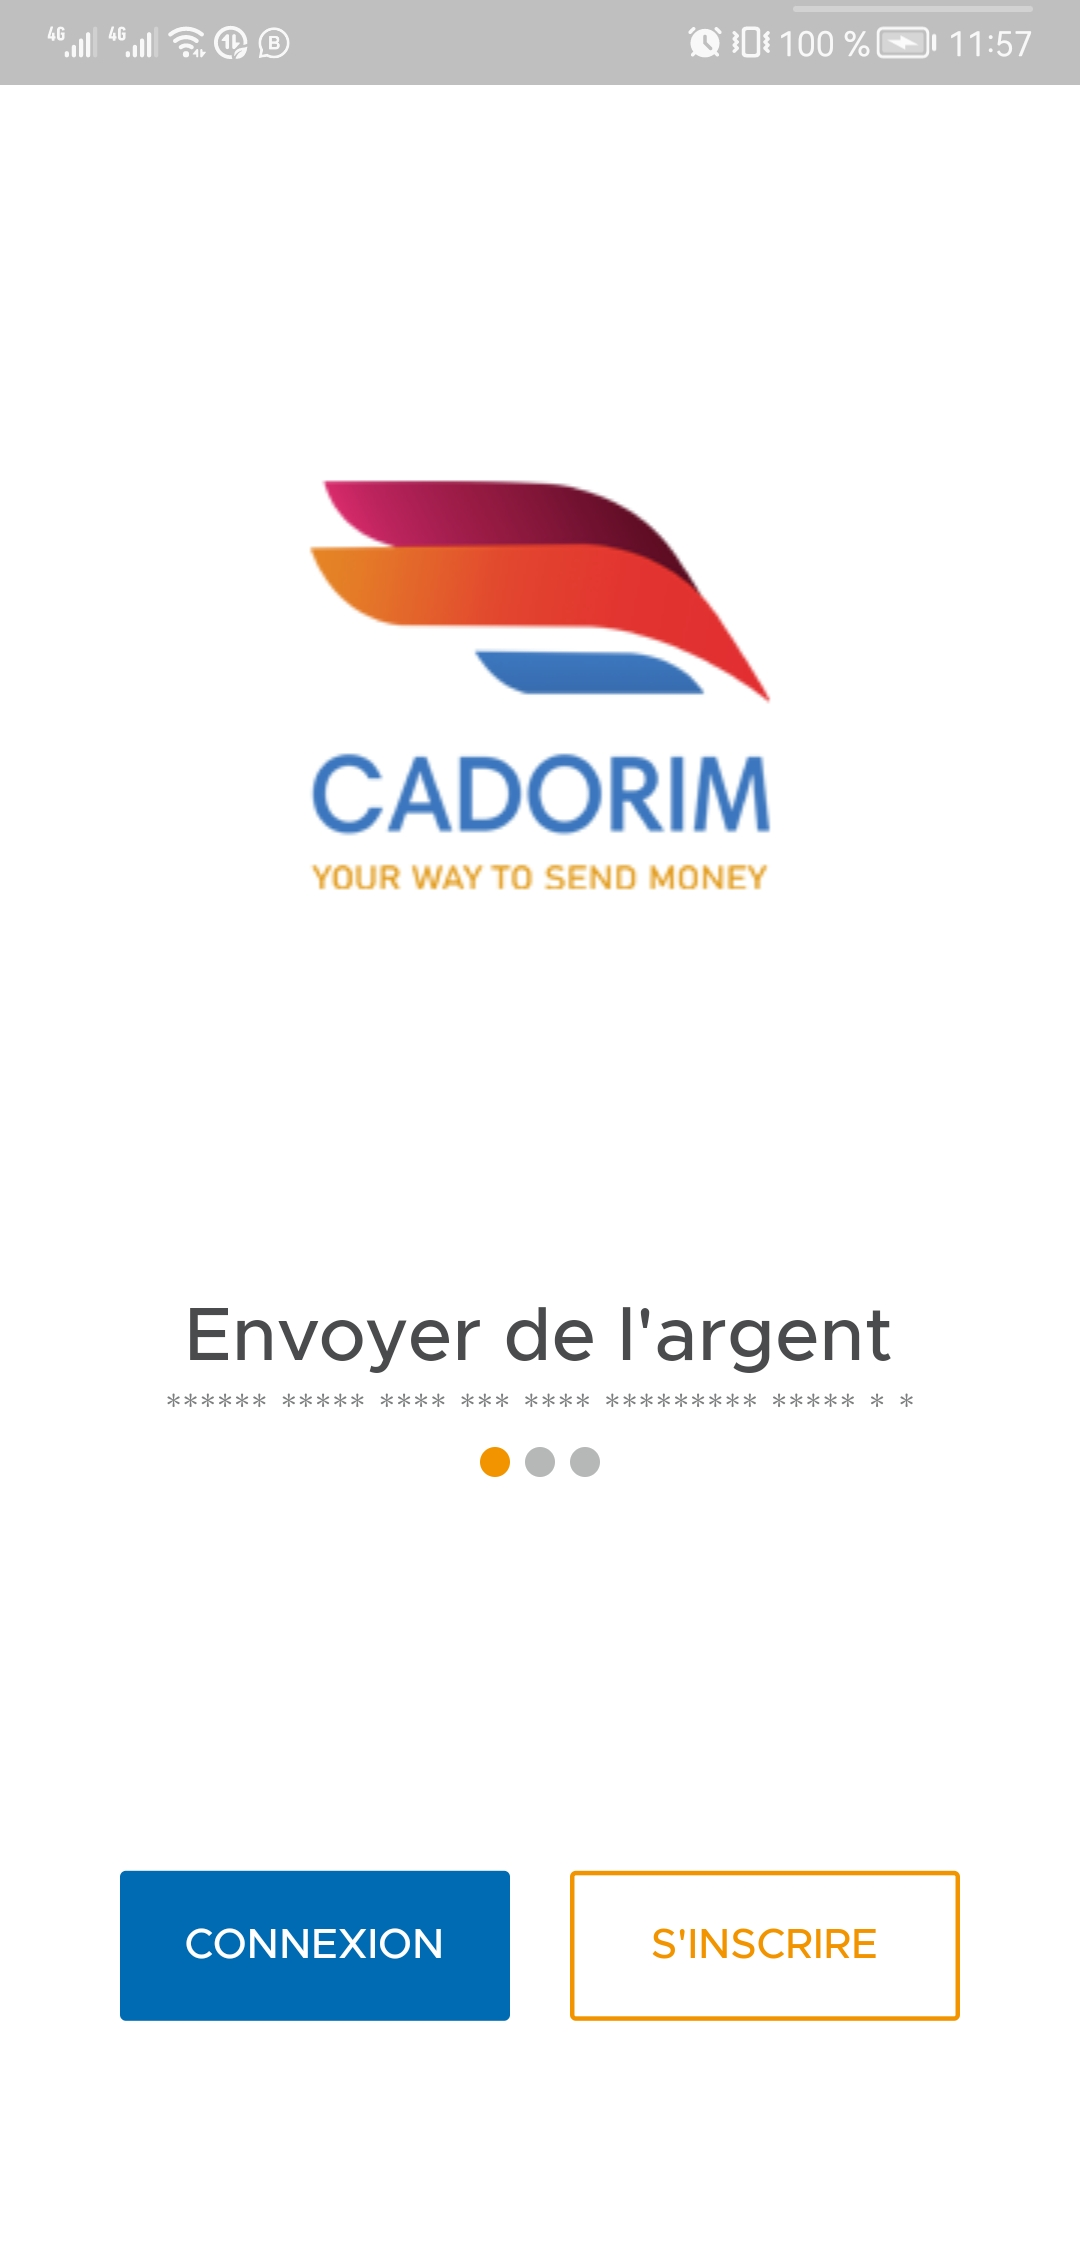
\includegraphics[width=\hsize, valign=m]{./Template LaTeX/Images/2.jpg}
		\caption{Interfaces Accueil}
		\label{fig.painel_sicapi}
	\end{subfigure}
	\caption{Interfaces d'acceil}
	\label{fig.sicapi}
\end{figure}
\begin{comment}
	
\begin{figure}%
	\centering
	\subfloat[\centering choix de lange ]{{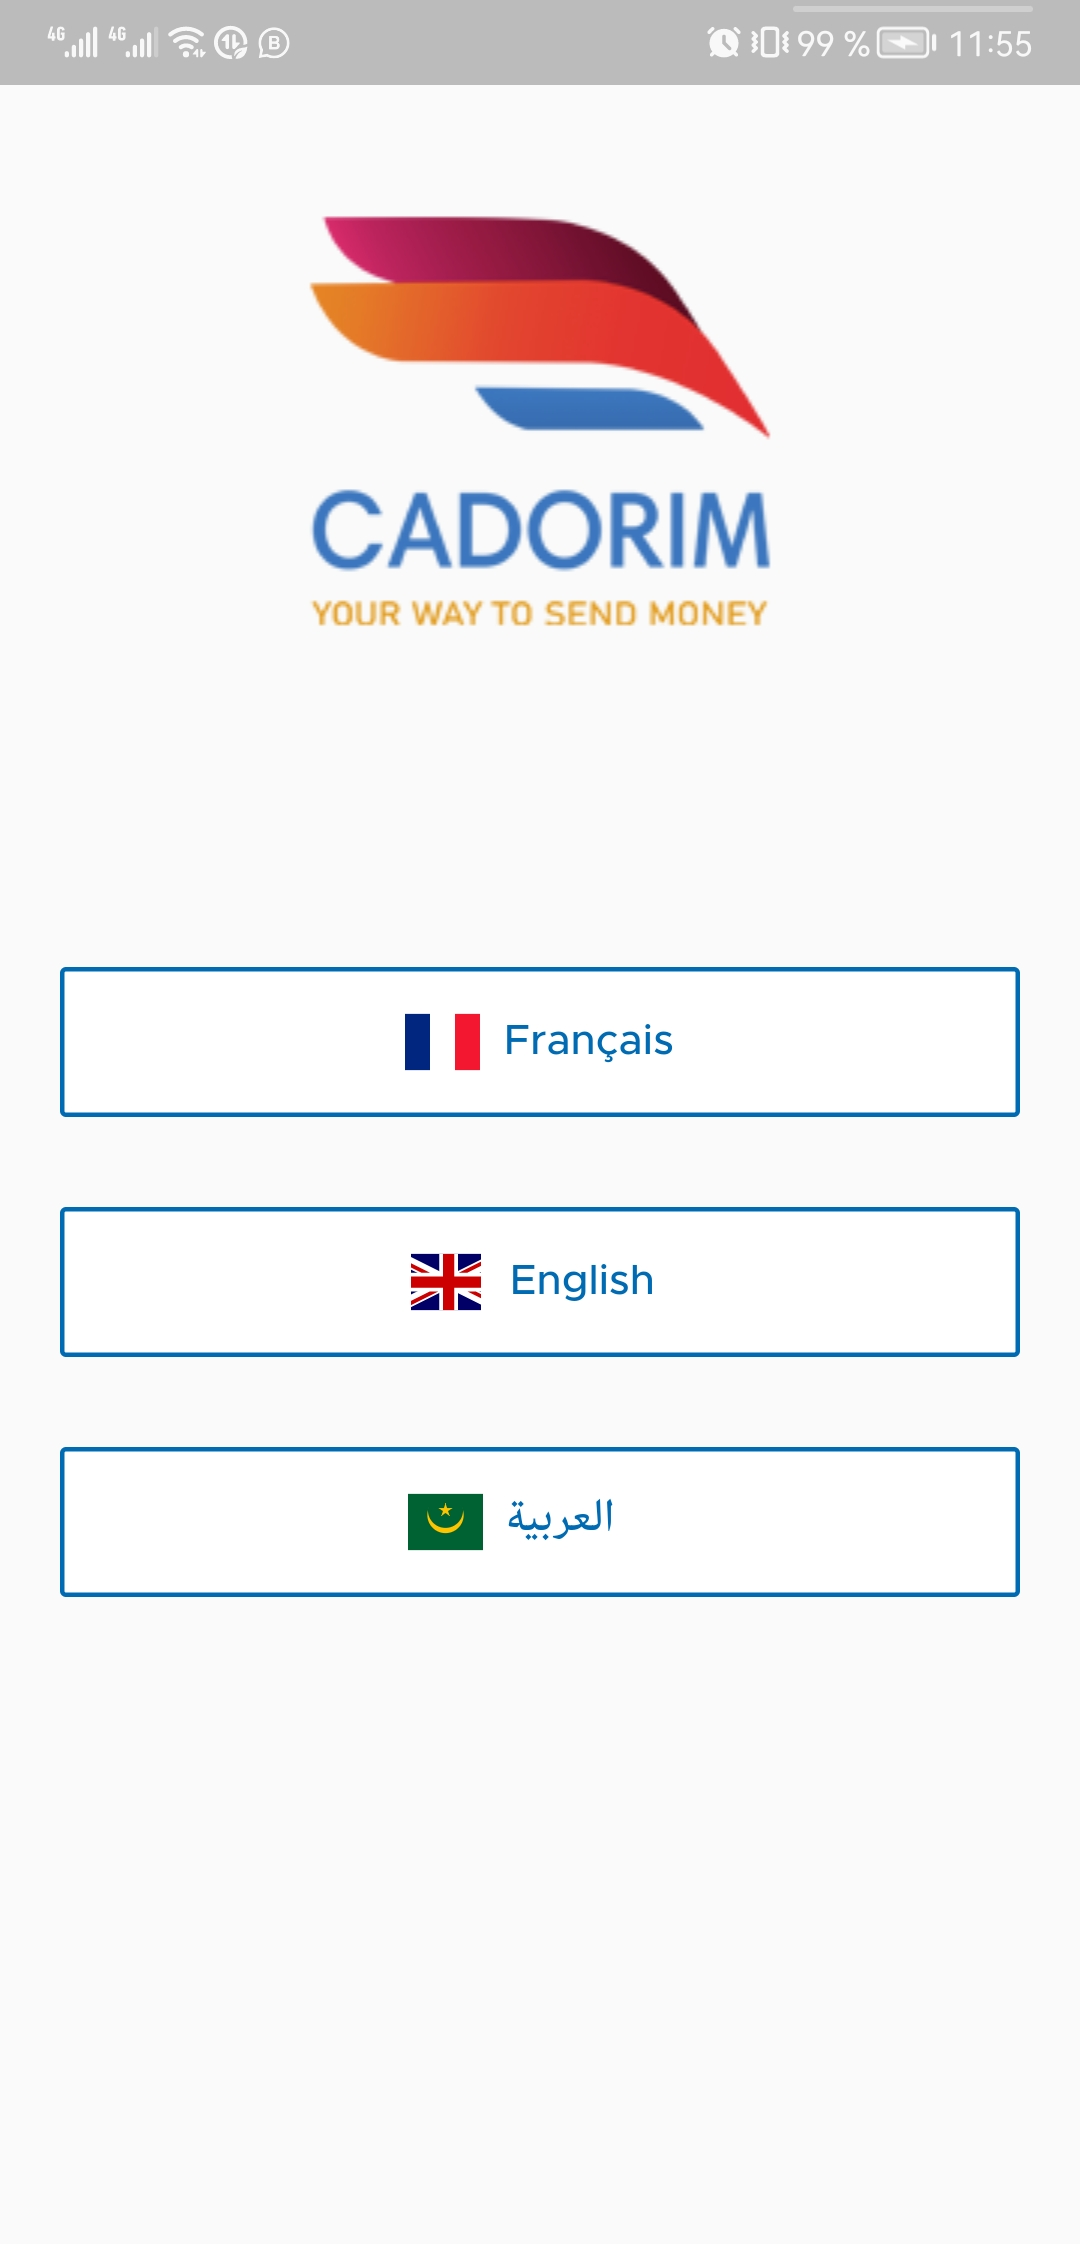
\includegraphics[width=5cm]{./Template LaTeX/Images/1.jpg} }}%
	\qquad	
	\subfloat[\centering  Acceuil]{{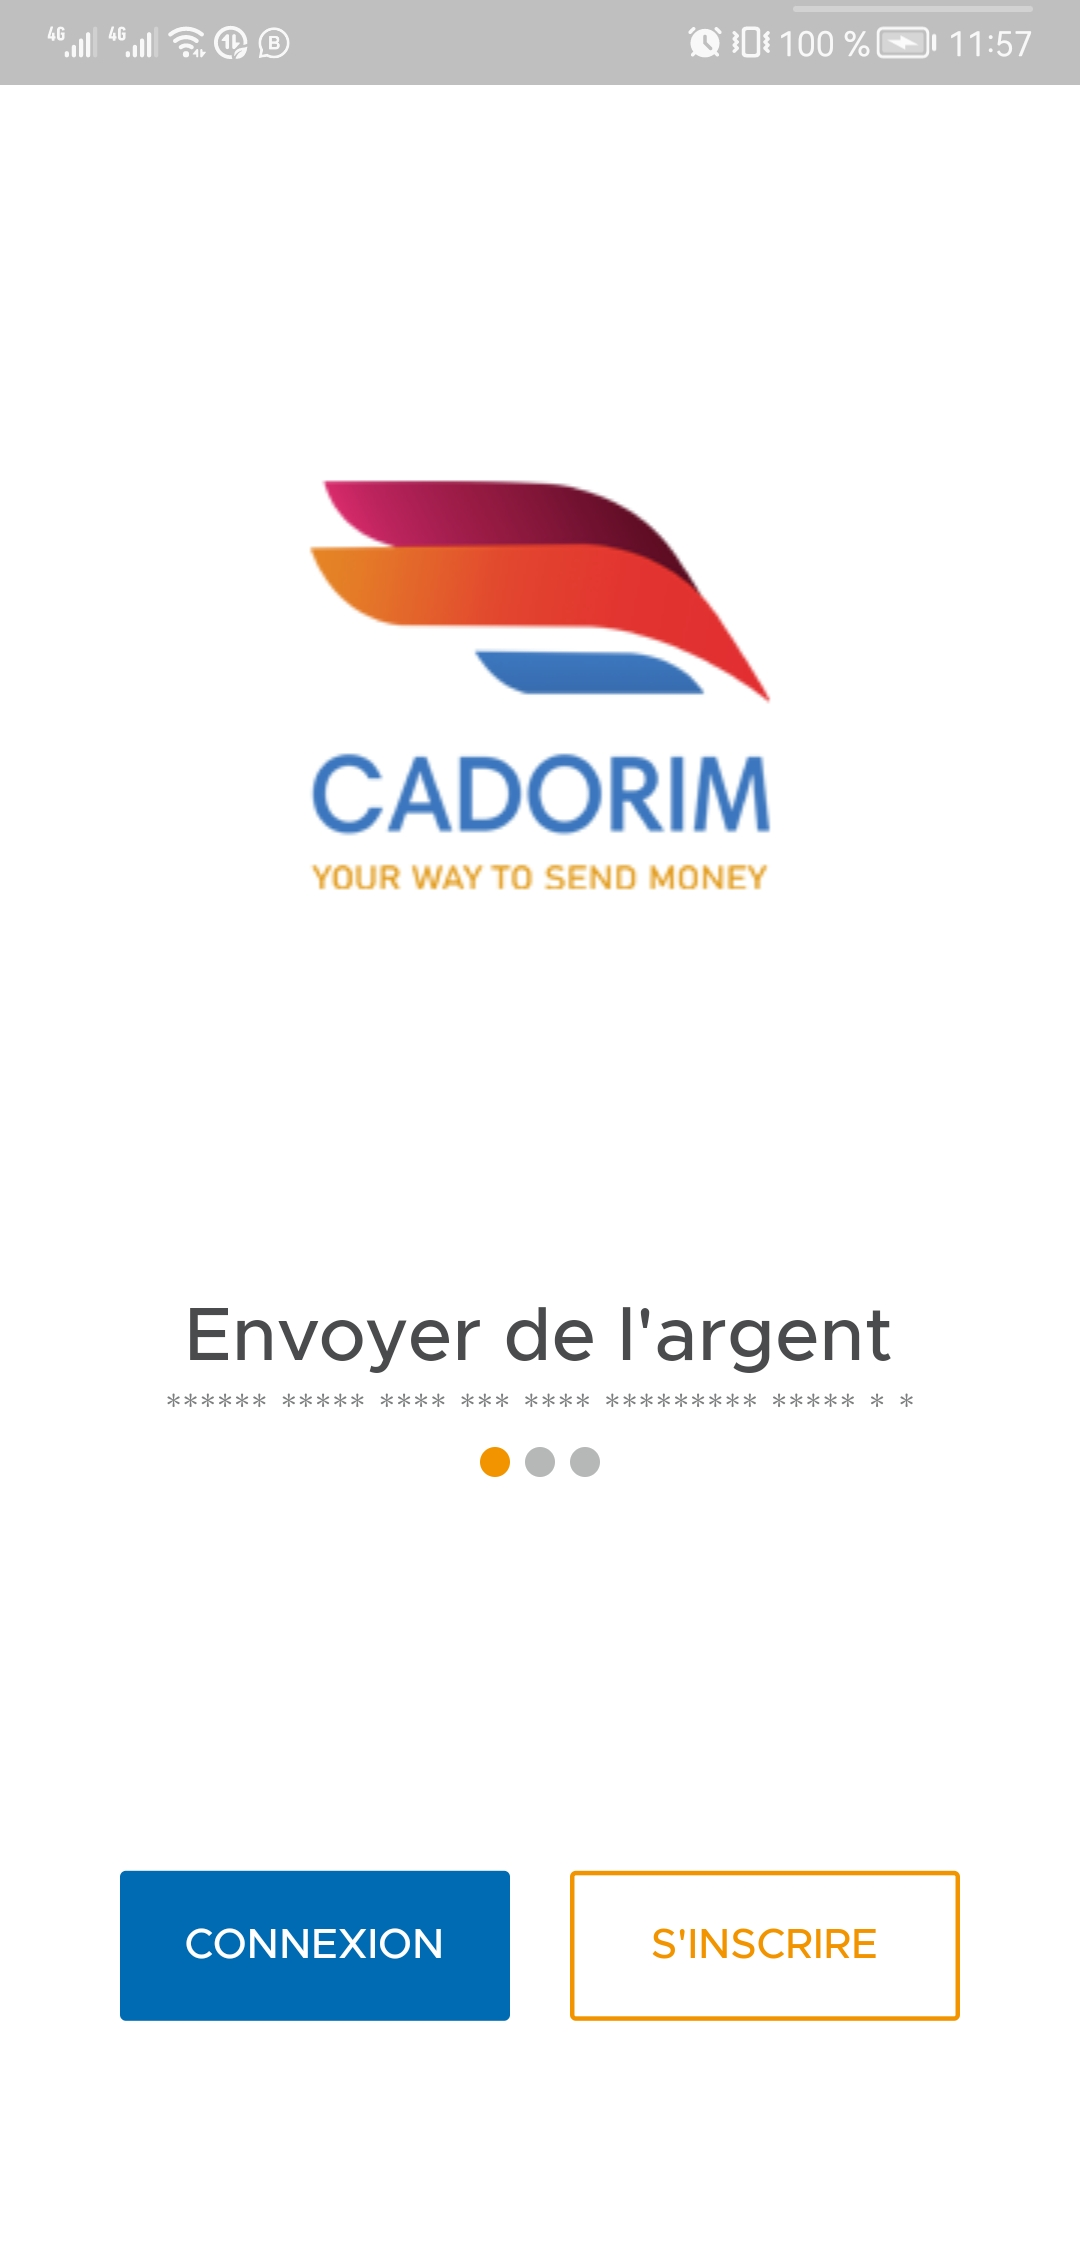
\includegraphics[width=5cm]{./Template LaTeX/Images/2.jpg} }}%
	\caption{Interfaces Accueil}%
	\label{fig:example}%
\end{figure}


	content...

\begin{figure}%
	\centering
	\subfloat[\centering choix de lange ]{{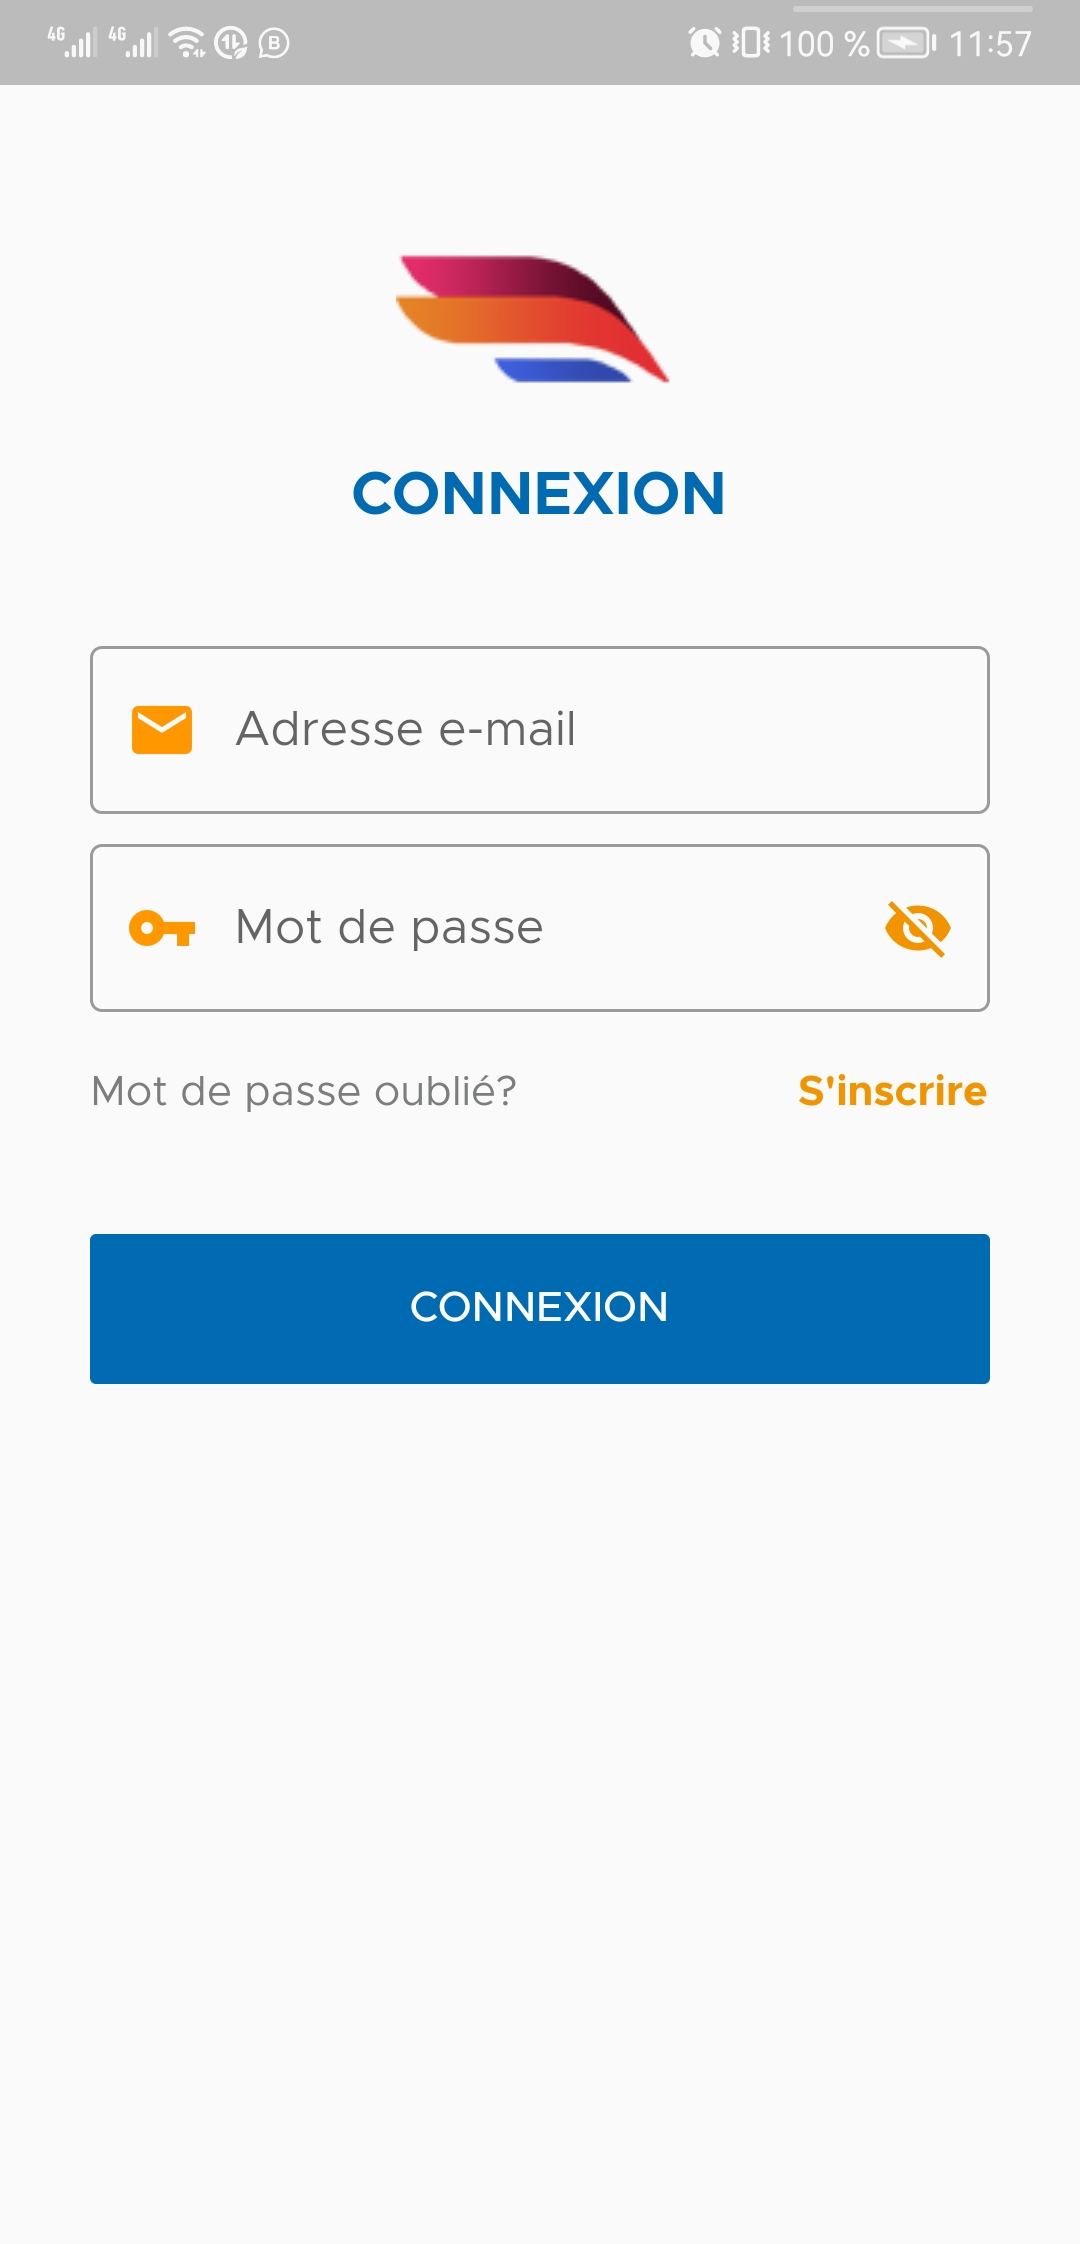
\includegraphics[width=5cm]{./Template LaTeX/Images/3.jpg} }}%
	\qquad
	\subfloat[\centering  Acceuil]{{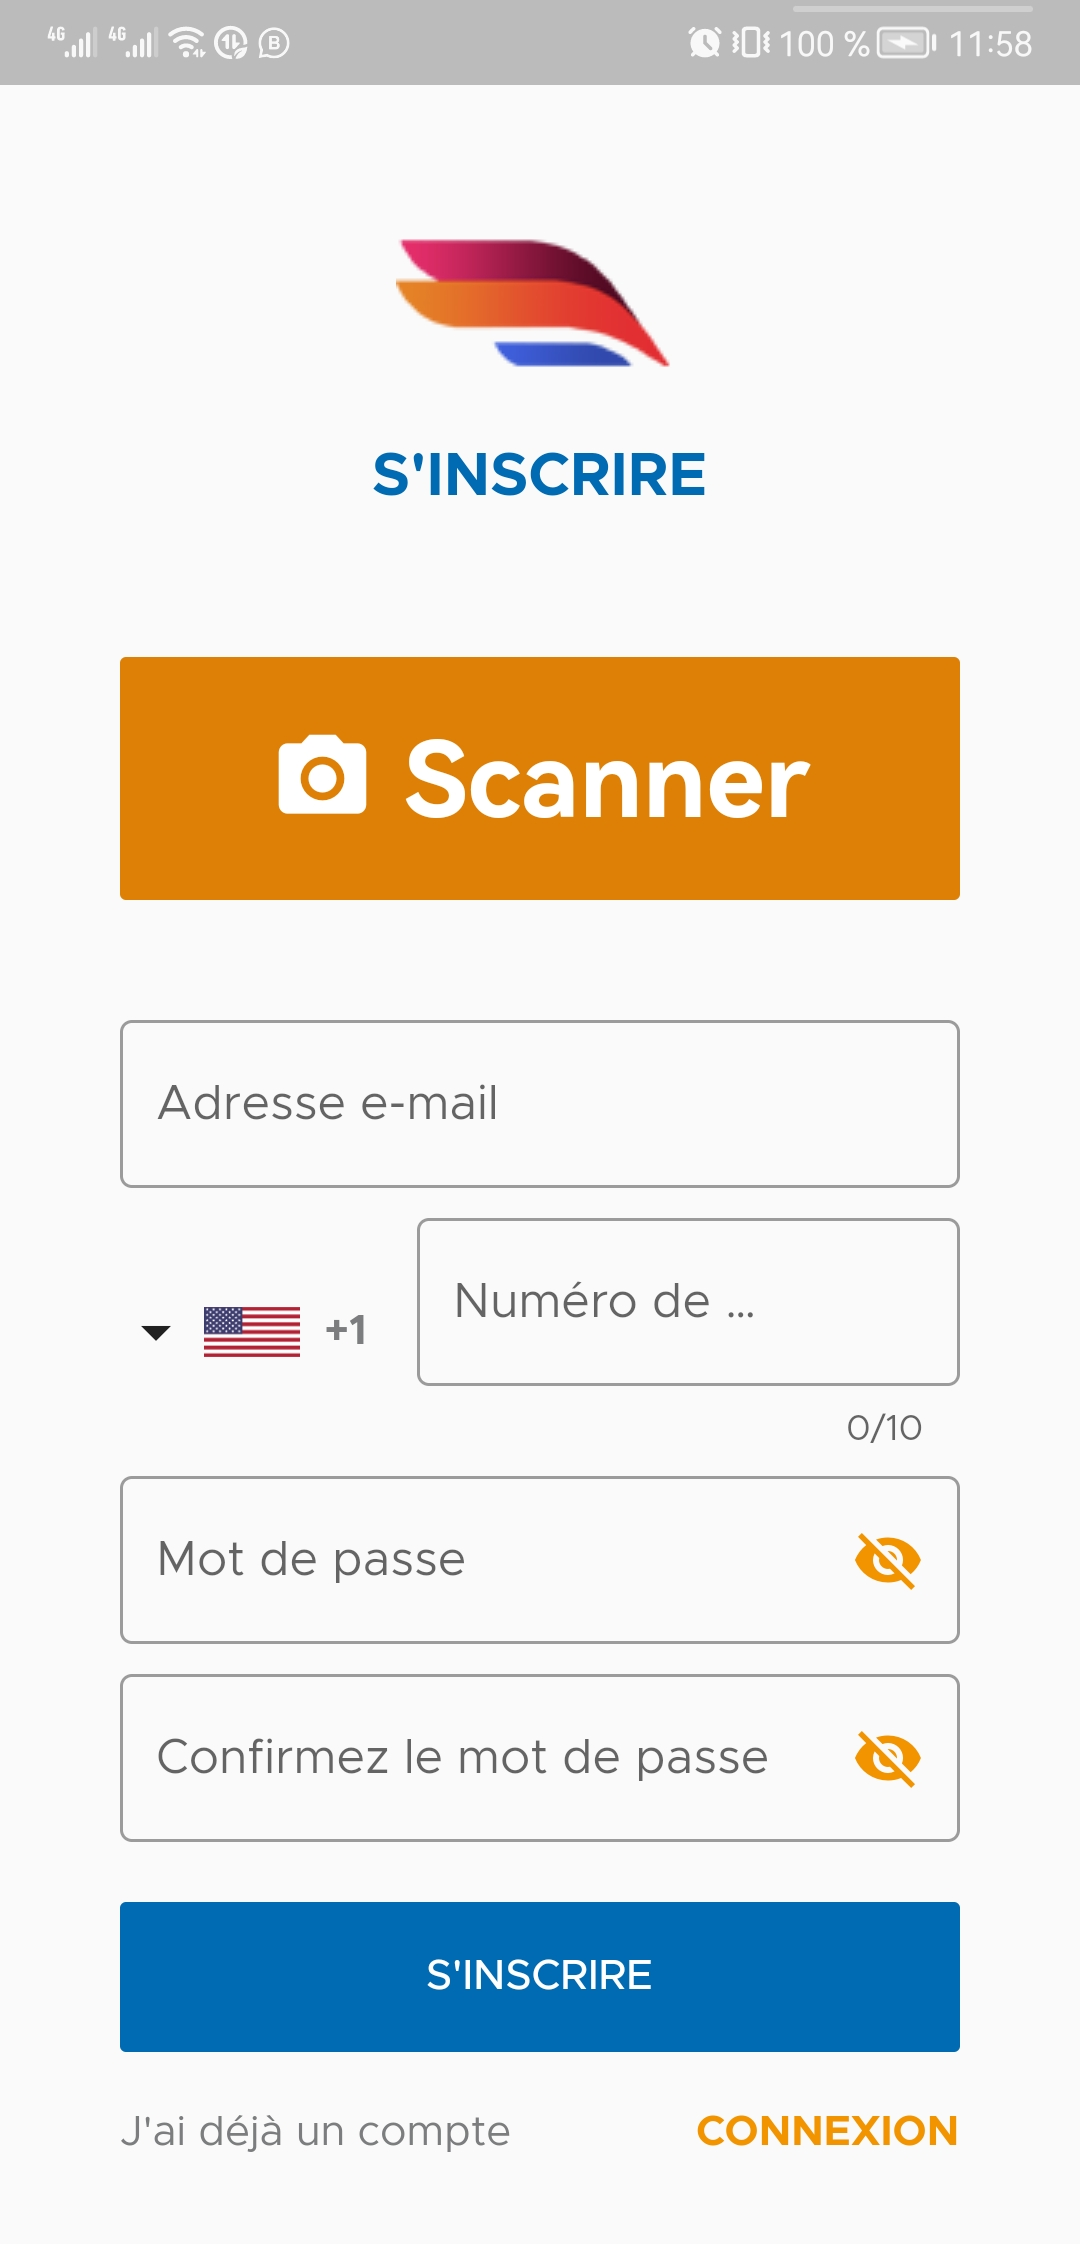
\includegraphics[width=5cm]{./Template LaTeX/Images/4.jpg} }}%
	\caption{Interfaces Accueil}%
	\label{fig:example}%
\end{figure}
\end{comment}

	%\chapter{Interface et utilisation de l'application}
\label{sec:Interface}	
\end{document}